\documentclass[conference]{IEEEtran}
\IEEEoverridecommandlockouts
% The preceding line is only needed to identify funding in the first footnote. If that is unneeded, please comment it out.
\usepackage{cite}
\usepackage{longtable}
\usepackage{amsmath,amssymb,amsfonts}
\usepackage{algorithmic}
\usepackage{graphicx}
\usepackage{textcomp}
\usepackage{xcolor}
\def\BibTeX{{\rm B\kern-.05em{\sc i\kern-.025em b}\kern-.08em
    T\kern-.1667em\lower.7ex\hbox{E}\kern-.125emX}}
\begin{document}

\title{Implementation and Simulation of Simplified Necessary Components of a Classic CPU*\\
{\footnotesize \textsuperscript{*}Note: Project of the course ICE3405P-Computer Organization}
}

\author{\IEEEauthorblockN{Nan Lin}
\IEEEauthorblockA{\textit{SPEIT} \\
\textit{Shanghai Jiao Tong University}\\
Shanghai, China \\
lns\_brandon@sjtu.edu.cn}
\and
\IEEEauthorblockN{Yanxu Meng}
\IEEEauthorblockA{\textit{SPEIT} \\
\textit{Shanghai Jiao Tong University}\\
Shanghai, China \\
meng-mou-xu@sjtu.edu.cn}
}

\maketitle

\begin{abstract}
This document is a model and instructions for \LaTeX.
This and the IEEEtran.cls file define the components of your paper [title, text, heads, etc.]. *CRITICAL: Do Not Use Symbols, Special Characters, Footnotes, 
or Math in Paper Title or Abstract.
\end{abstract}

\begin{IEEEkeywords}
component, formatting, style, styling, insert
\end{IEEEkeywords}


\section{Question 1-5: Implementation of a Two's Complement Calculation}

\subsection{Question 1}\label{sec:q_A}

The two's complement of a binary number is obtained by following the rule:
\begin{itemize}
    \item If the sign bit (highest bit) is 0, it indicates that the sign-magnitude representation is a positive number. In this case, the binary number is unchanged.
    \item If the sign bit is 1, we should invert its digits and add one to the least significant bit. 
\end{itemize}

This method allows for binary arithmetic and simplifies the design of digital circuits for arithmetic operations.
A straightforward implementation is to adopt different operation modes depending on the sign bit using a multiplexer. A typical multiplexer is shown in Figure~\ref{fig:multiplexer}. For an 8-bit binary number, suppose that it could be represented as:
\begin{equation}
    \overline{s_7 s_6 s_5 s_4 s_3 s_2 s_1 s_0}
\end{equation}

$s_7$ is the sign bit, therefore playing the role of Select for all other bits ($s_0$ to $s_6$) here.

\begin{figure}[h!]
    \centering
    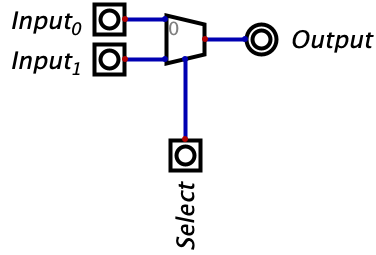
\includegraphics[width=0.3\textwidth]{assets/multiplexer.png}
    \caption{A Multiplexer. When Select is 0, the output corresponds to the value of $\text{Input}_0$, neglecting the condition of $\text{Input}_1$. Inversely, when Select is 1, the output corresponds to the value of $\text{Input}_1$.}
    \label{fig:multiplexer}
\end{figure}

In order to add one to the least significant bit, an adder is required.
A half-adder is a fundamental component in digital arithmetic. It takes two single-bit binary inputs and produces a sum and carry output. The truth table for a half-adder is shown below:

\begin{table}[h!]
\centering
\begin{tabular}{|c|c|c|c|}
\hline
A & B & Sum (Result) & CarryOut \\ \hline
0 & 0 &  0  &   0   \\ \hline
0 & 1 &  1  &   0   \\ \hline
1 & 0 &  1  &   0   \\ \hline
1 & 1 &  0  &   1   \\ \hline
\end{tabular}
\caption{Truth table for a half-adder}
\end{table}

The corresponding half-adder circuit diagram is illustrated in Figure~\ref{fig:half_adder}.

\begin{figure}[h!]
\centering
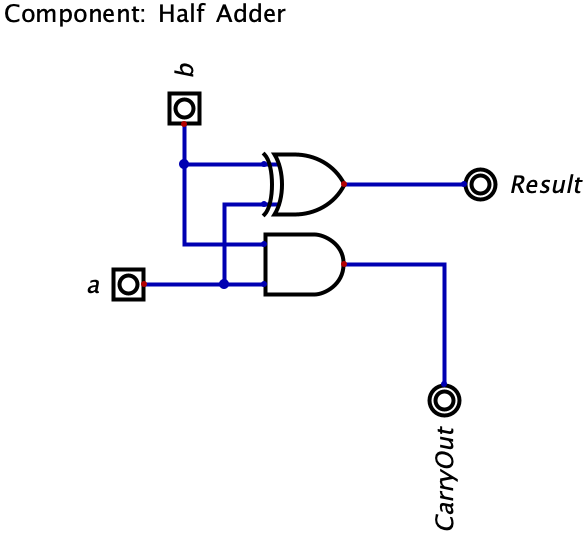
\includegraphics[width=0.4\textwidth]{assets/half_adder.png}
\caption{Half-Adder Circuit}
\label{fig:half_adder}
\end{figure}

We use a half-adder rather than a full adder for multiple reasons:
\begin{itemize}
    \item A half-adder has a relatively simpler structure. Most importantly, its depth is one less than a full adder and it contains fewer gates which provides the advantage of lower energy consumption and less time consumption.
    \item A half-adder is proved to be effective because to implement a two's complement circuit, we only need to calculate $\overline{s_6 \dots s_0} + \overline{0 \dots 01}$ (taking 8-bit binary numbers as an example). Since all the 
    bits are 0, we can put the CarryOut onto the place of another adder.
\end{itemize}

To implement an 8-bit two's complement circuit, we combine multiple half-adders; each half-adder is used to calculate the corresponding bit of the binary number. The process involves inverting each bit of the input number and then adding one using a series of adders. The detailed circuit diagram is shown in Figure~\ref{fig:twos_complement}.



\begin{figure}[h!]
\centering
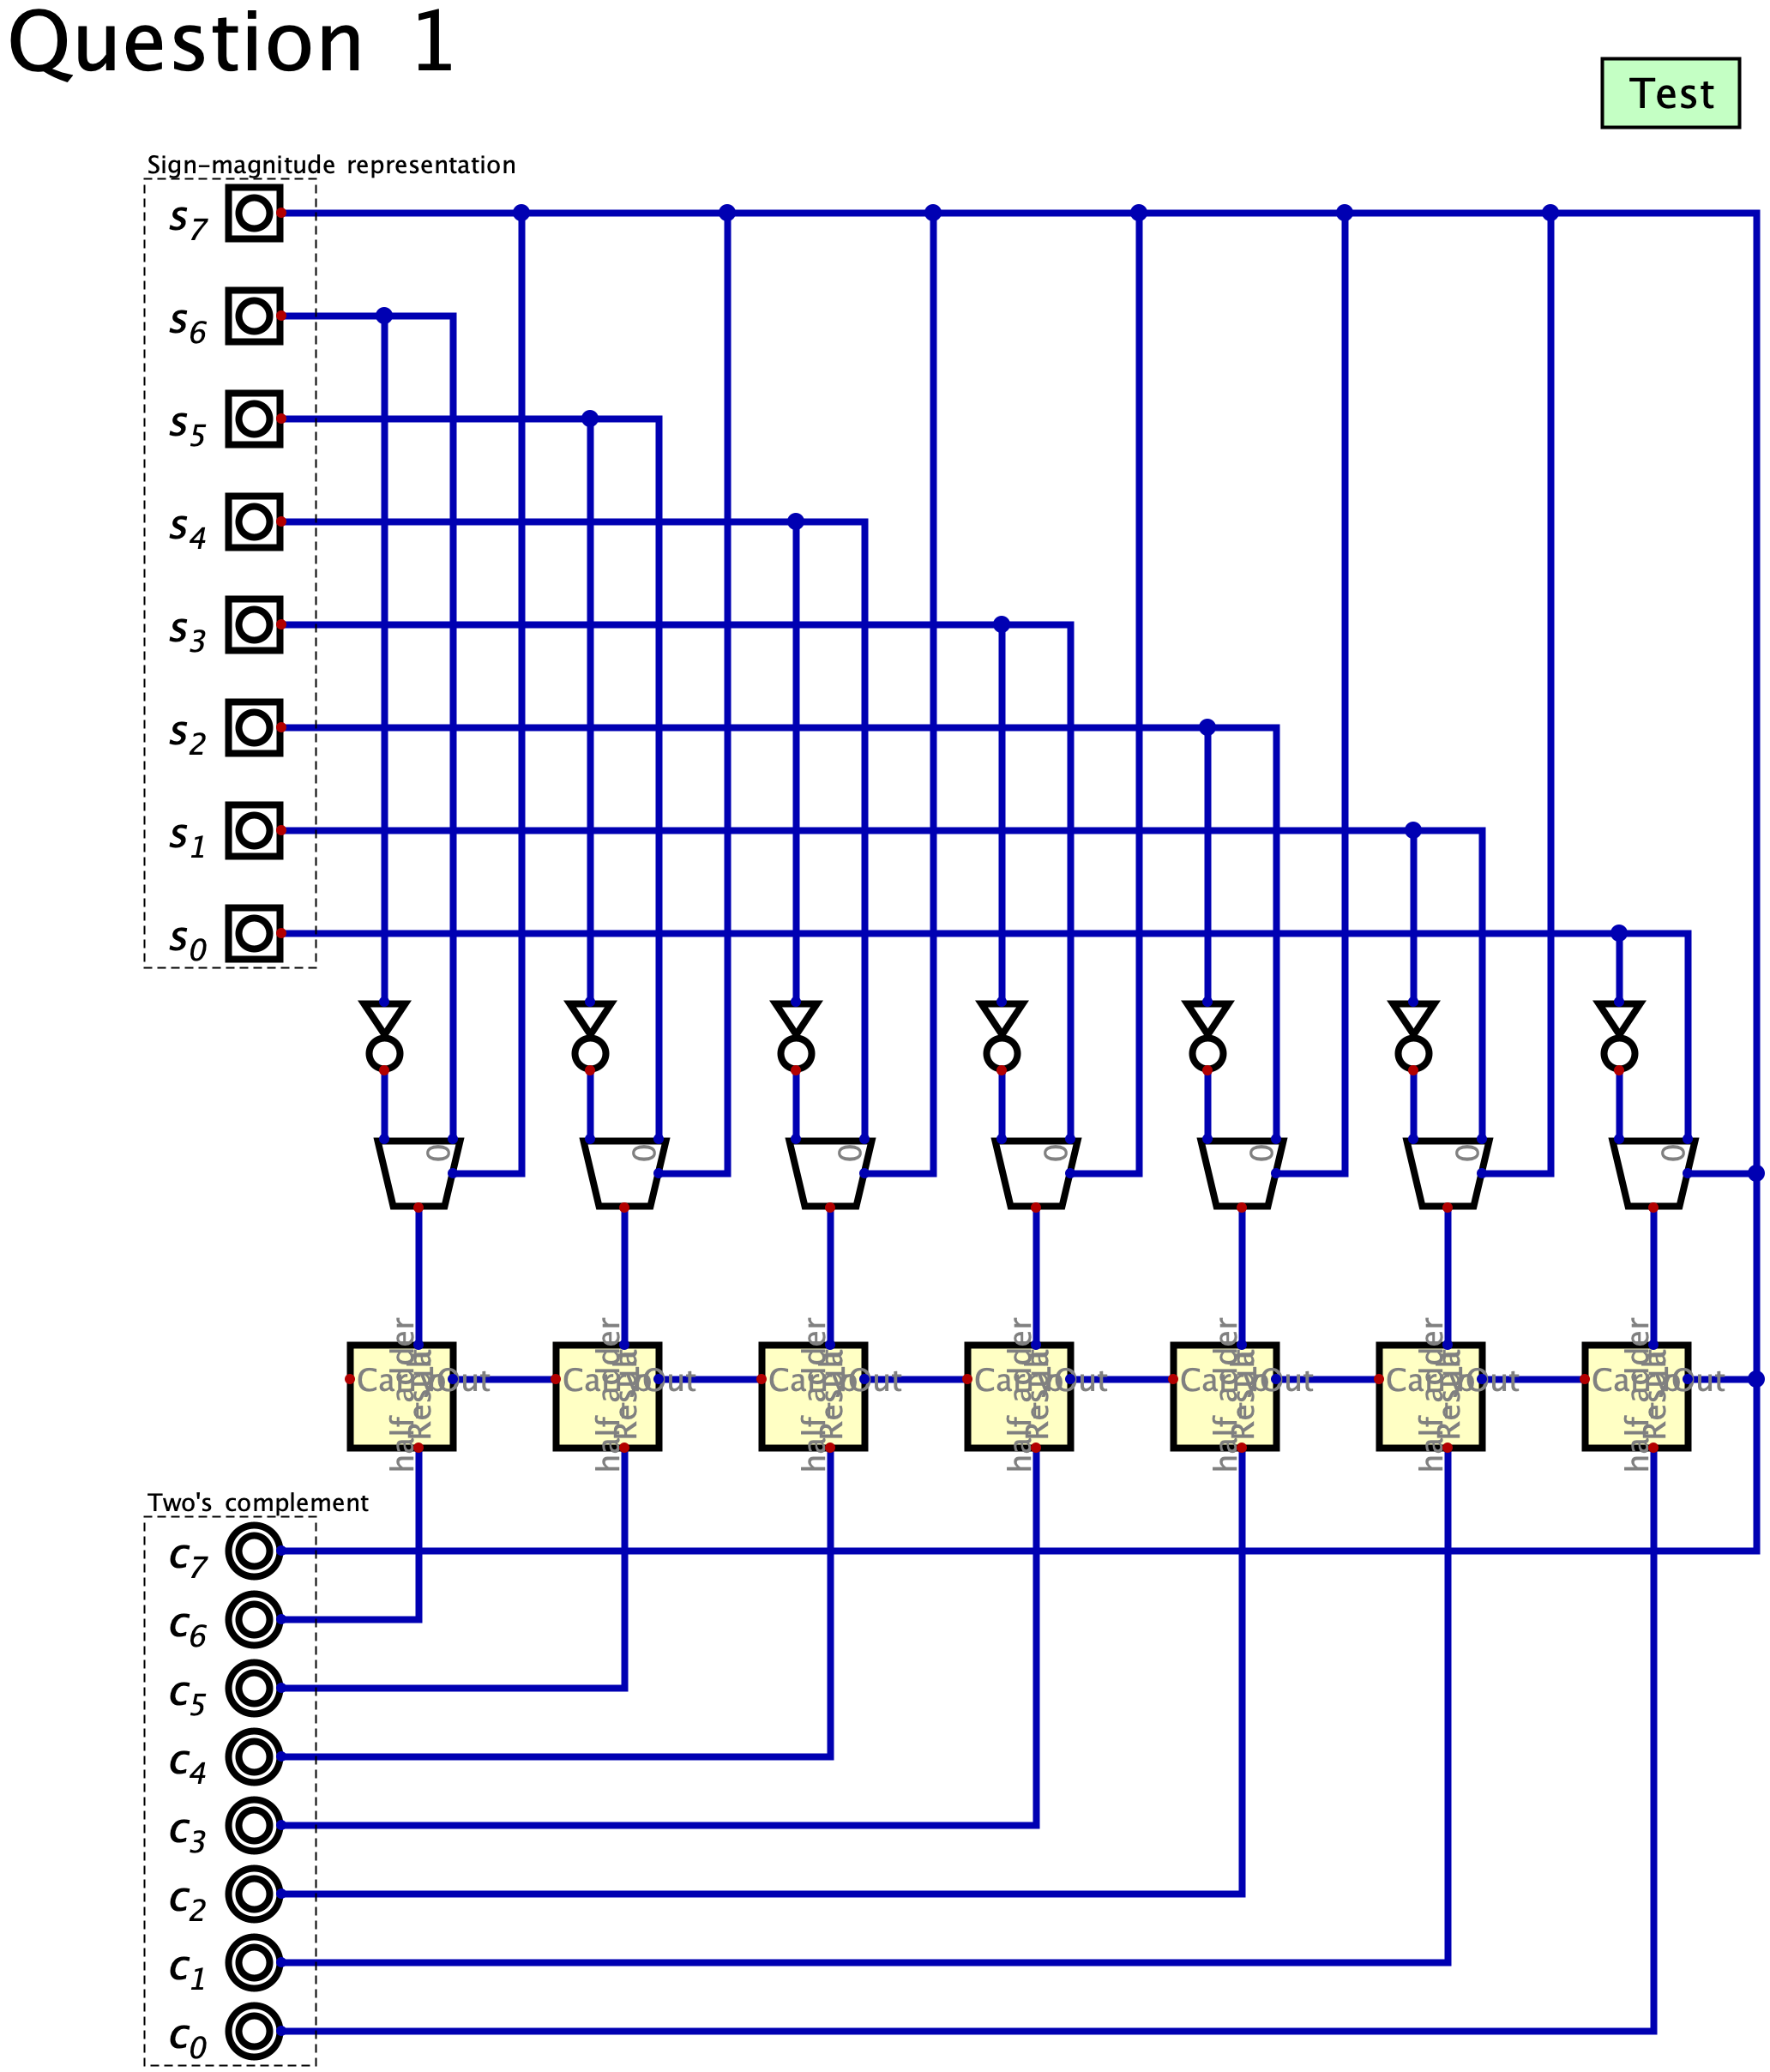
\includegraphics[width=0.45\textwidth]{assets/twos_complement.png}
\caption{8-bit Two's Complement Circuit. The yellow box is a half-adder implemented in Figure~\ref{fig:half_adder}}
\label{fig:twos_complement}
\end{figure}


\subsection{Question 2}

To analyze the depth and complexity of the two's complement circuit for 8 bits, we divide the process into two stages.

The first stage is the \textbf{inversion stage}. Each bit requires a NOT gate, thus in the first stage:
\begin{itemize}
\item Depth: 1 (because all of the NOT gates operate simultaneously)
\item Complexity: 7 (NOT gates)
\end{itemize}

The second stage is the \textbf{addition stage}. For each bit, a half-adder is applied.
The depth of each half-adder is 1 and the complexity is 2. Since there are 7 bits that need to be calculated one by one, in the second stage:
\begin{itemize}
    \item Depth: $7 \times 1 = 7$
    \item Complexity: $7 \times 2 = 14$
\end{itemize}

Summing up the two stages, the depth of calculation of the two's complement of an 8-bit binary number is $1 + 7 = 8$ and the complexity is $7 + 14 = 21$.

We expand the results to any $2^p$-bit ($p \in \mathbb{N}$) two's complement circuit.

\begin{enumerate}
\item In the \textbf{inversion stage}, the depth is 1 due to parallelization, and the complexity is $2^p - 1$.
\item In the \textbf{addition stage}, the depth is $2^p - 1$ and the number of gates required is $2 \times (2^p - 1)$.
\end{enumerate}

\textbf{
Conclusion: For a $2^p$-bit two's complement circuit, the depth is $2^p$, and the complexity is $3(2^p - 1)$.
}

\subsection{Question 3}

In order to reduce the depth of the circuit, having a closer look at the circuit implemented in Section~\ref{sec:q_A}, the main problem is that the CarryOut is passed on in series.
In other words, to calculate the two's representation of $s_k$ of a $2^p$-bit binary number ($0 < k \leq 2^p-2$), we have to wait for the values of $k-1$ CarryOuts one by one.

To optimize this process, we first propose a new version of the two's complement circuit for an 8-bit machine by employing a method that uses two 4-bit lookahead carry adders in series. This approach allows for the calculation of four bits and their carry at once, then passing the carry to the next set of four bits. This reflects the divide and conquer strategy.

\subsubsection{Two 4-bit Lookahead Adders in Series}\label{sec:3-A}

The implementation involves the following steps:
\begin{enumerate}
    \item \textbf{Inversion Stage}: This stage is unchanged, where each of the 8 bits is inverted using NOT gates.
    \item \textbf{Addition Stage}: The 8-bit addition is divided into two 4-bit additions using lookahead carry adders.
    \begin{itemize}
        \item \textbf{First 4-bit Adder}: Computes the result and the carry for the first four bits.
        \item \textbf{Second 4-bit Adder}: Computes the result for the next three (but not four!) bits.
    \end{itemize}
\end{enumerate}

We then implement a classical 4-bit lookahead carry adder which can be found in textbooks. First, we introduce two fundamental components.

In digital circuits, the Generate-Propagate (GP) logic is used to speed up the carry calculation in adders. For two binary inputs $A_i$ and $B_i$, the generate ($G_i$) and propagate ($P_i$) signals are defined as:
\begin{equation}
g_i = a_i \cdot b_i
\end{equation}
\begin{equation}
p_i = a_i + b_i
\end{equation}
The GP generator is used to generate respectively the AND and OR results of two variables, this result will be exploited later on.
The implementation of the GP generator is displayed in Figure~\ref{fig:gp_generator}. For any bit, the value is 
\begin{equation}
    \forall k \in [\![1, 2^p-2]\!], \quad s_k = a_k + b_k + c_{k-1}
\end{equation}
where $c_{k-1}$ is the carry bit into position $k$.

\begin{figure}[h!]
\centering
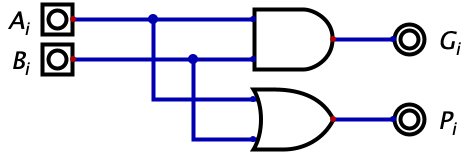
\includegraphics[width=0.4\textwidth]{assets/generate_gp.png}
\caption{GP Generator Circuit}
\label{fig:gp_generator}
\end{figure}

The carry bits can be calculated as follows:

\begin{equation}\label{eq:carry-bit}
    c_{i+1} = a_i b_i + (a_i + b_i) c_i
\end{equation}

due to the reason that the carry bit is 1 if

\begin{itemize}
    \item Both of the two bits are $1$
    \item Any of the two bits is $1$ and the carry bit from the former bit is 1.
\end{itemize}

Here we replace $a_ib_i$ and $a_i + b_i$ with $g_i$ and $p_i$. The Equation~\ref{eq:carry-bit} turns into:

\begin{equation}\label{eq:carry-bit-deduction}
    c_{i+1} = g_i + p_i c_i
\end{equation}

We therefore deduce all the carry bits based on Equation~\ref{eq:carry-bit-deduction}:
\begin{align}
    c_1 &= g_0 + p_0 c_0 \label{eq:temp1}\\
    c_2 &= g_1 + p_1 c_1 = g_1 + p_1 g_0 + p_1 p_0 c_0 \\
    c_3 &= g_2 + p_2 c_2 = g_2 + p_2 g_1 + p_2 p_1 g_0 + p_2 p_1 p_0 c_0 \\
    c_4 &= g_3 + p_3 c_3 = g_3 + p_3 p_2 g_1 + p_3 p_2 p_1 g_0 + p_3 p_2 p_1 p_0 c_0 \label{eq:temp2}
\end{align}




A full adder also takes the CarryIn of the former bit compared to a half adder. It is displayed in Figure~\ref{fig:full_adder}. 


\begin{figure}[h!]
    \centering
    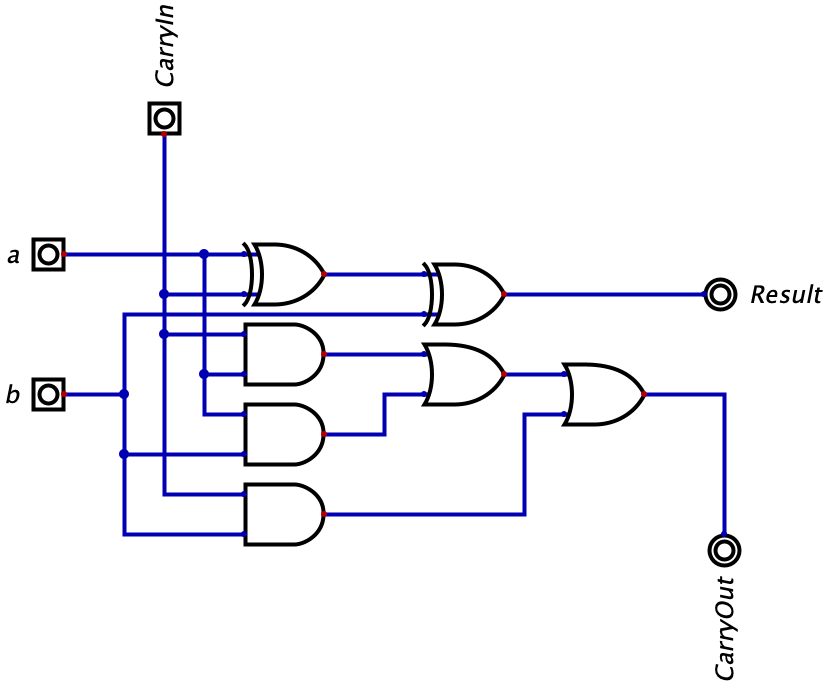
\includegraphics[width=0.5\textwidth]{assets/full_adder.png}
    \caption{Full-Adder Circuit}
    \label{fig:full_adder}
\end{figure}

A classic 4-bit lookahead carry adder based on full adders is shown in Figure~\ref{fig:lca}. We then combine the two 4-bit adders in series. The final two's complement circuit is shown in Figure~\ref{fig:tc-dq}. When the
sign bit is 1, it implies that we should invert its digits and add one to the least significant bit. In this case, the sign bit is passed to the first CarryIn input, and the operation of the full adder is identical to:
\begin{align}\label{eq:carry-bits-result}
    \overline{a_3 a_2 a_1 a_0} &+ \overline{0000} \quad \text{with CarryIn } 1 \\
    \overline{0 a_6 a_5 a_4} &+ \overline{0000} \quad \text{with CarryIn from the former 4-bit adder}
\end{align}

\begin{figure}[h!]
    \centering
    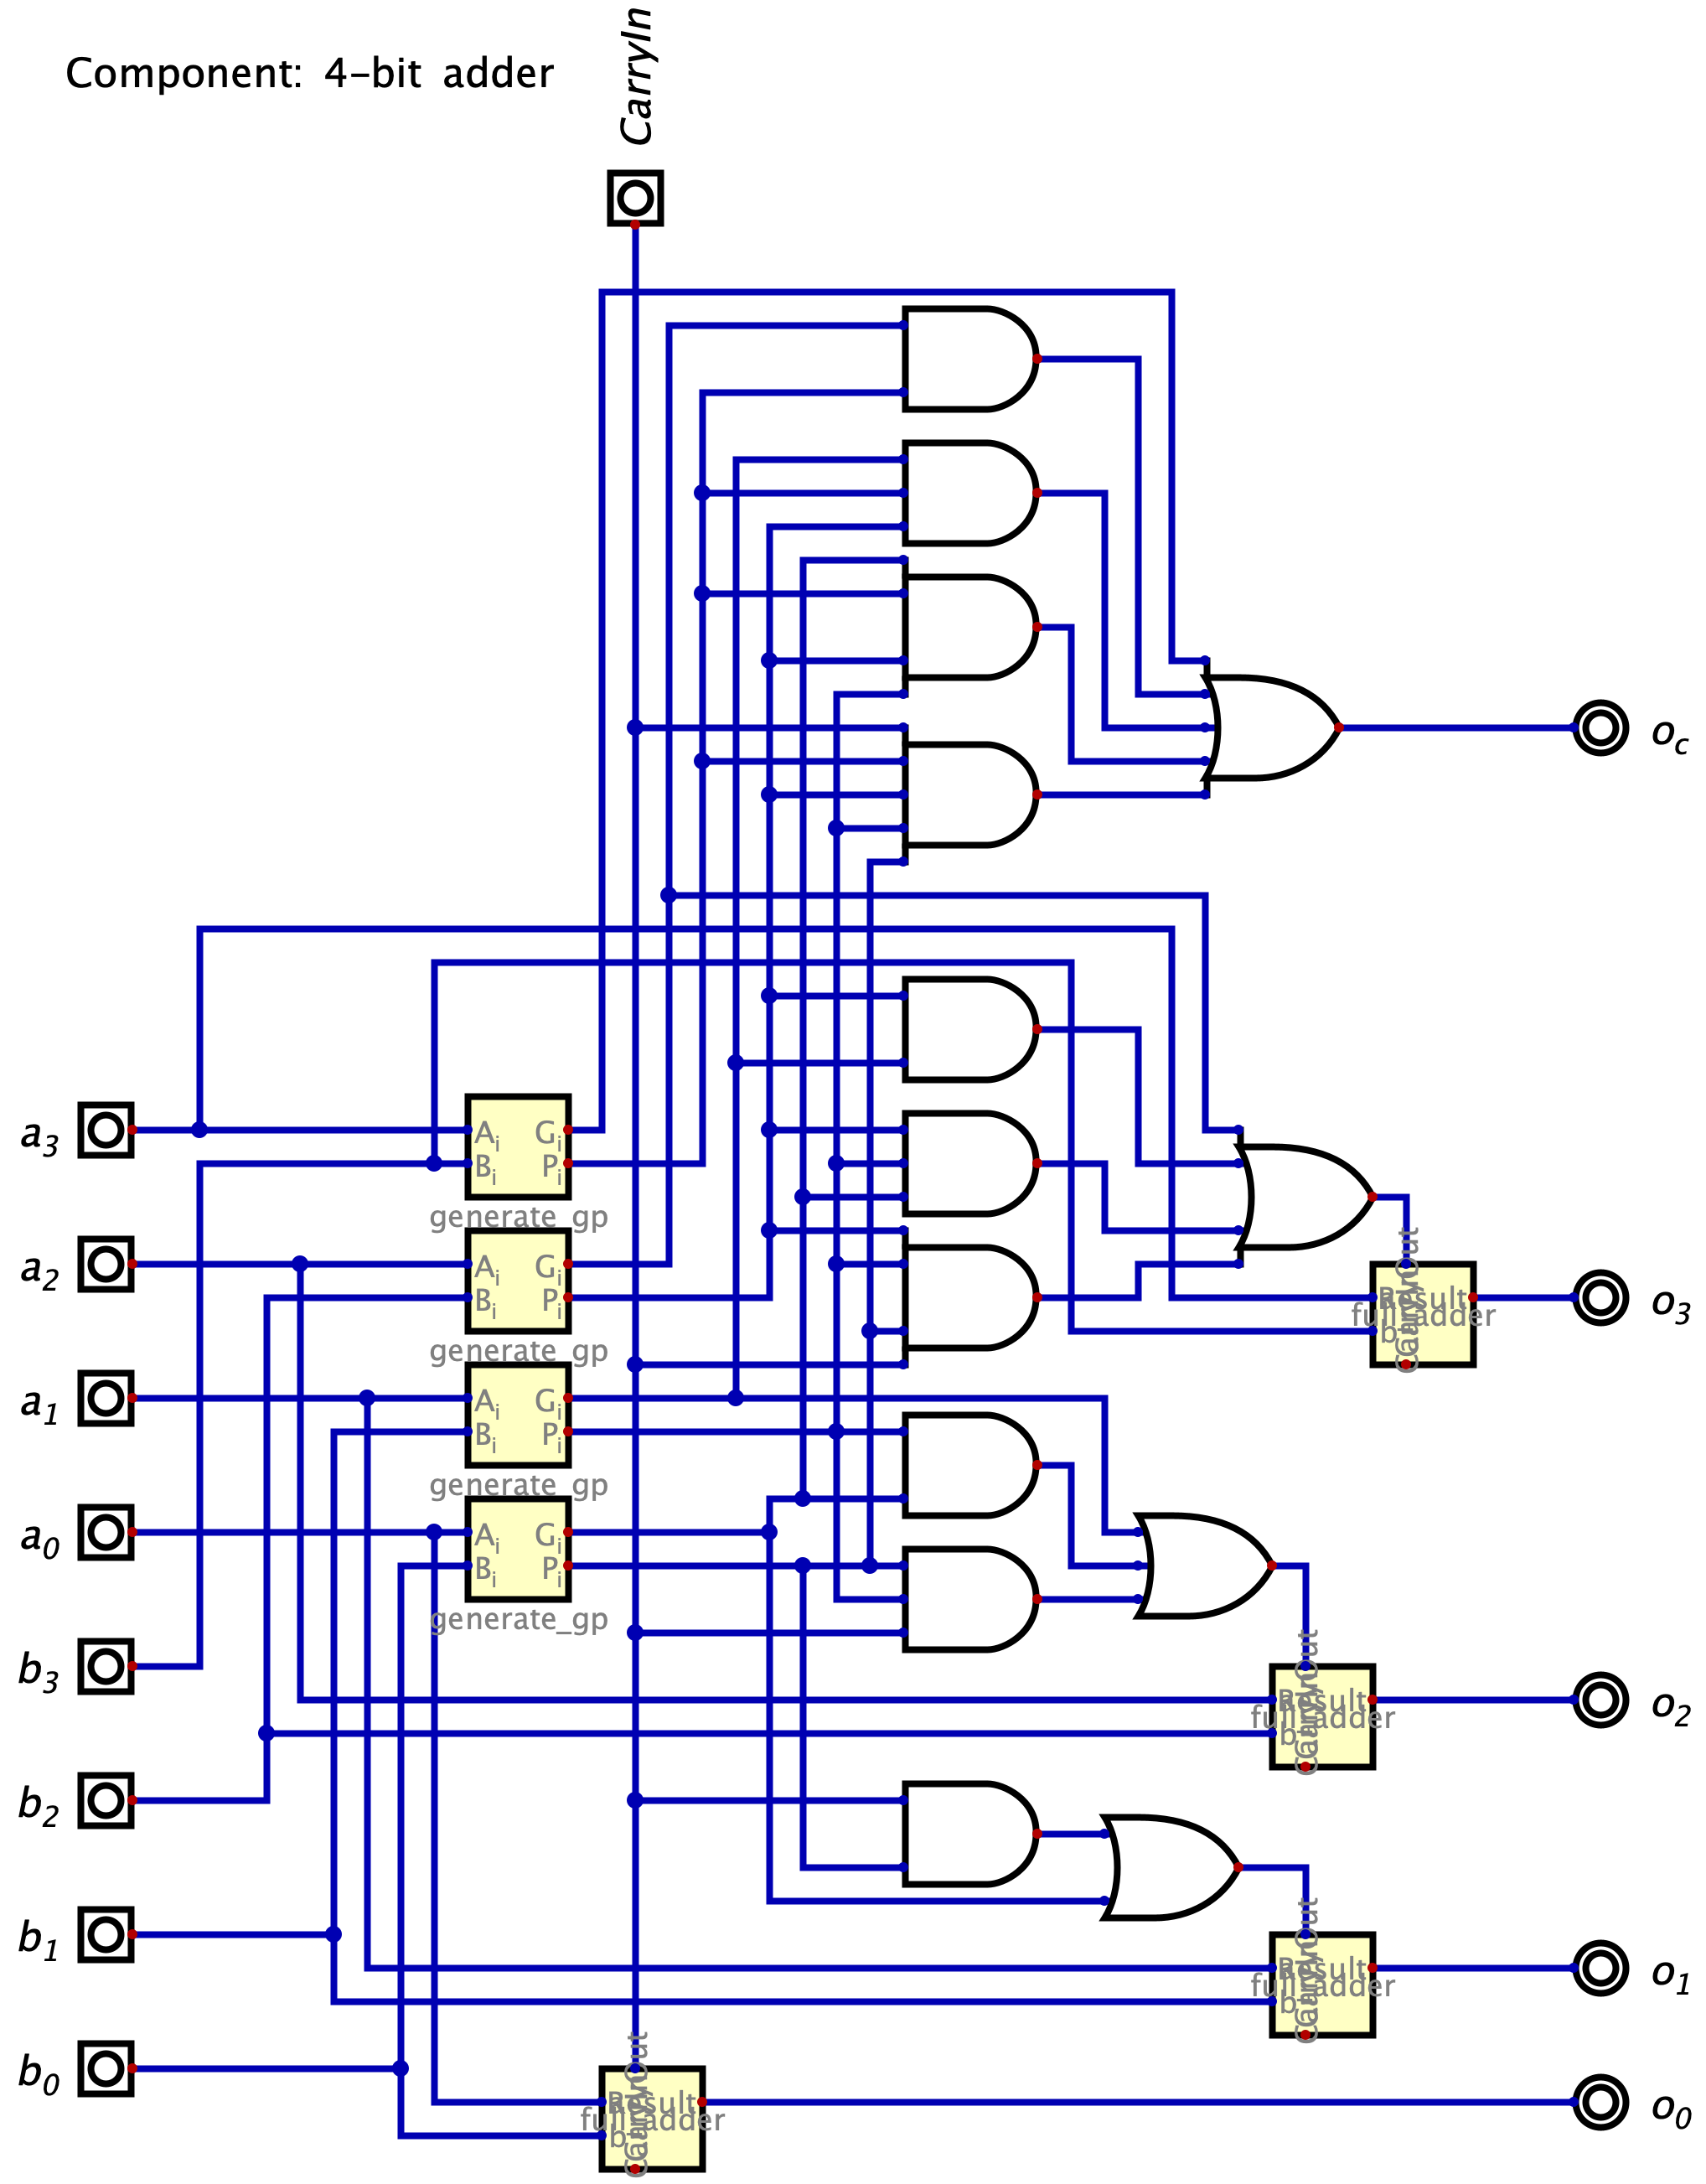
\includegraphics[width=0.5\textwidth]{assets/adder_4bits.png}
    \caption{4-bit Lookahead Carry Adder based on Full-Adders}
    \label{fig:lca}
    \end{figure}


    \begin{figure}[h!]
        \centering
        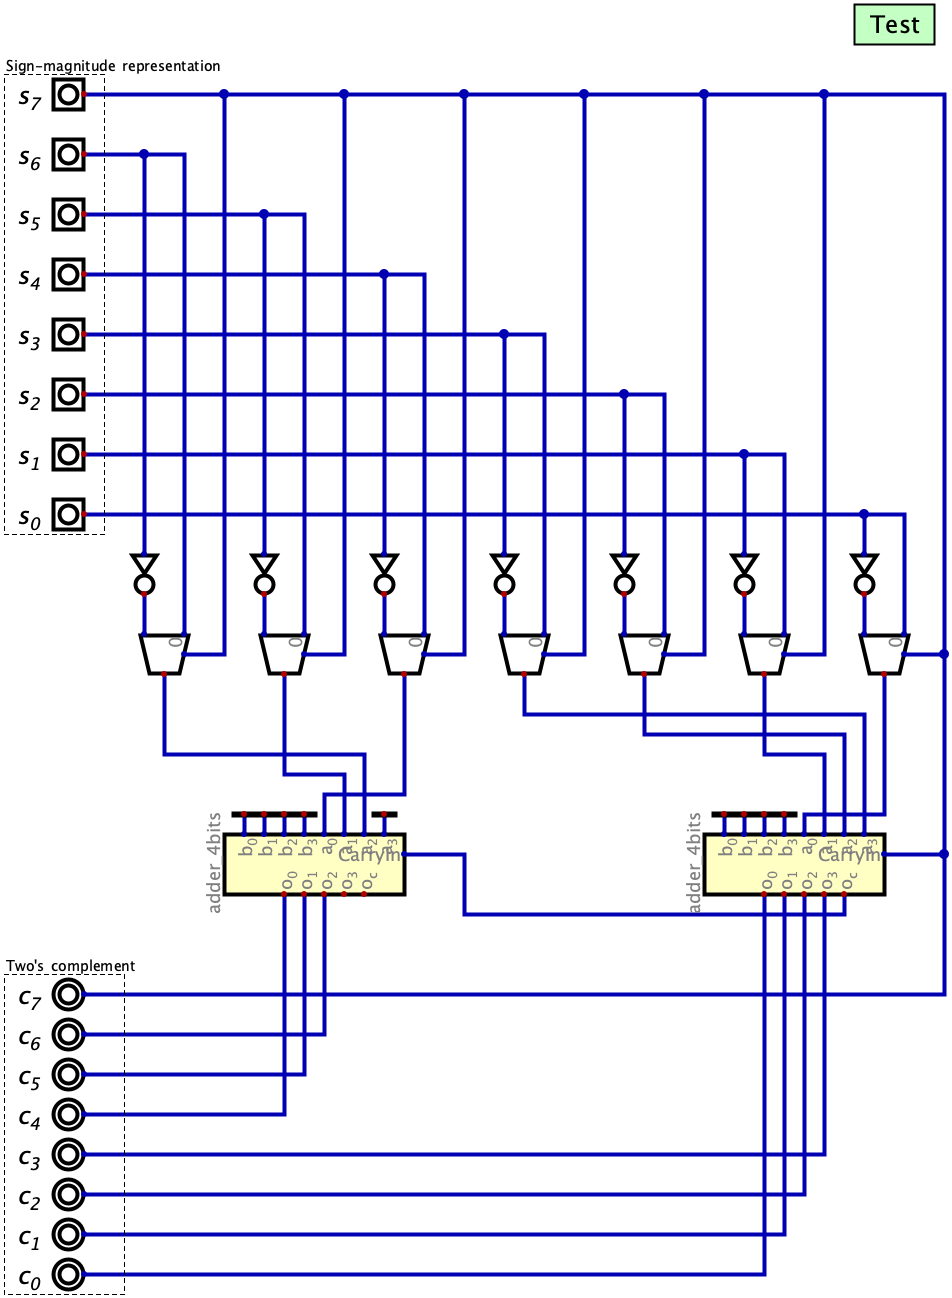
\includegraphics[width=0.45\textwidth]{assets/twos_complement_dq.png}
        \caption{8-bit Two's Complement Circuit (Divide and Conquer Method) Based on Full-Adders}
        \label{fig:tc-dq}
        \end{figure}

The reason why we put in series of 4-bit Lookahead Carry Adder instead of series of 8 (or even 16, 32, ...)-bit Lookahead Carry Adder is to reduce the complexity of designing the circuit.
As shown in Figure~{fig:lca}, to implement a 4-bit Lookahead Carry Adder, we need an AND gate with 5 inputs. This is already hard to fabricate in reality and it consumes much more time and energy if we separate the AND gates.

However, there are still spaces of optimization. This indeed is the implementation of a standard adder between two 8-bit binary numbers. Here, we're only required to perform addition on binary numbers with 1.
We could throw out 0s and full adders and adopt half adders.

Furthermore, since the other adder is always 0 in Equation~\ref{eq:carry-bits-result}, the G(enerate) signal is always 0. This implies for any valid value of $g_i$, they should be 0. Equations~\ref{eq:temp1} to~\ref{eq:temp2} could be transformed into:
\begin{align}
    c_1 &= p_0 c_0 \\
    c_2 &= p_1 p_0 c_0 \\
    c_3 &= p_2 p_1 p_0 c_0 \\
    c_4 &= p_3 p_2 p_1 p_0 c_0
\end{align}

Based on these two points, the 4-bit Lookahead Carry Adder could be optimized as shown in Figure~\ref{fig:lca-optimize}.


\begin{figure}[h!]
    \centering
    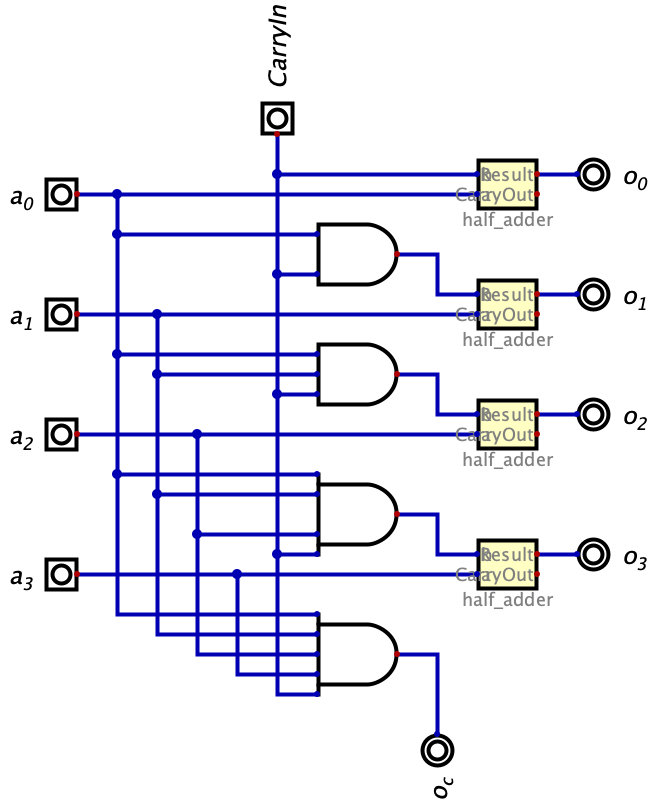
\includegraphics[width=0.45\textwidth]{assets/adder_4bits_copy.png}
    \caption{Optimized 4-bit Lookahead Carry Adder based on Half-Adders and simplified gates}
    \label{fig:lca-optimize}
    \end{figure}

The corresponding 8-bit two's complement circuit is shown in Figure~\ref{fig:tc-dq-optimize}.


\begin{figure}[h!]
    \centering
    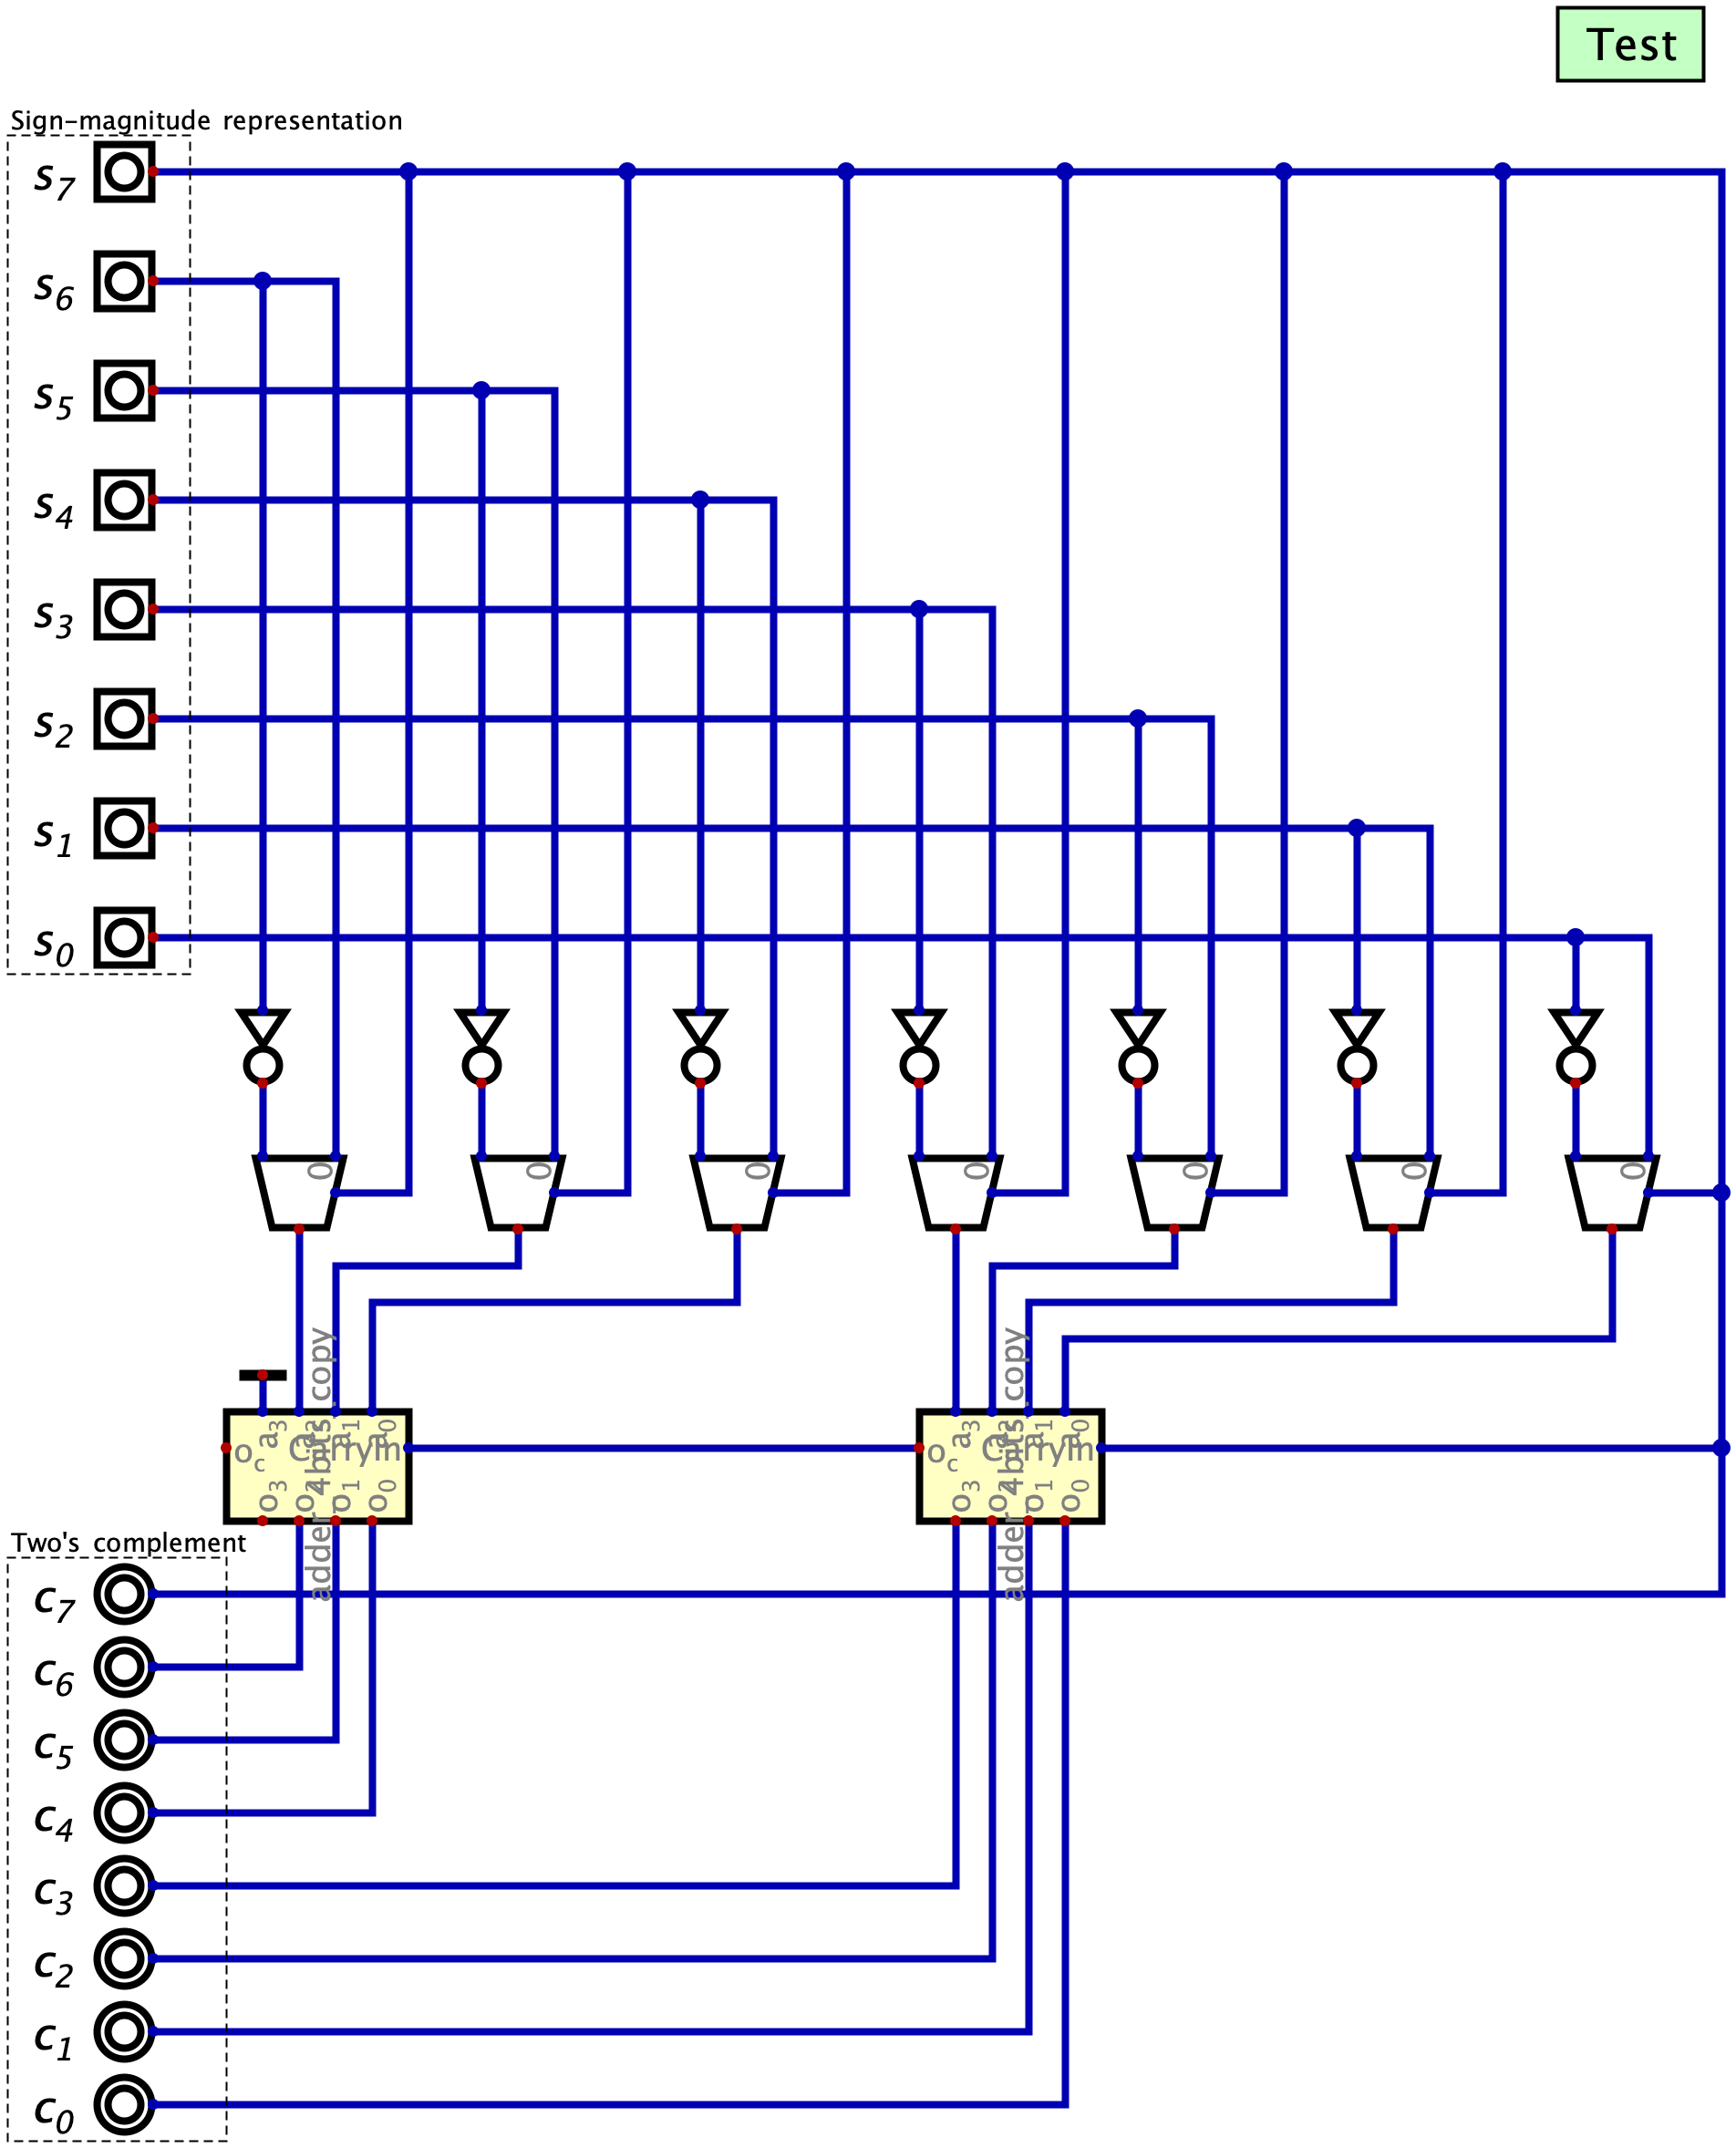
\includegraphics[width=0.45\textwidth]{assets/twos_complement_dq_copy.png}
    \caption{Optimized 8-bit Two's Complement Circuit (Divide and Conquer Method) Based on 4-bit Lookahead Carry Adder Proposed in Figure~\ref{fig:lca-optimize}}
    \label{fig:tc-dq-optimize}
    \end{figure}
It seems feasible for $p$ relatively small. However, if $p$ is much greater (e.g., to sum up two 64-bit binary numbers), the depth is still
comparatively high. Calculation of depth and complexity of this circuit is shown in Section~\ref{sec:q4}. The divide and conquer method is not fully implemented since we're only grouping up 4 bits together and then calculating them one by one. There are still spaces for improvement.


\subsubsection{Solution for binary numbers with much more bits}\label{sec:3-B}

A real divide and conquer solution is like this: we separate the bits into groups of 2 bits, calculate the values separately, then combine them into groups of 4 bits, then calculate the values separately, etc.

We analyze as follows (with some notations):
A 1-bit adder is: 
\begin{equation}
    a_0 + b_0 = \overline{r_0s_0} \quad \text{with}\quad \begin{cases}
        r_0 = a_0 \wedge b_0 \\
        s_0 = a_0 \oplus b_0
\end{cases}
\end{equation}

If we consider the carry from the former bit, knowing that 
\begin{equation}
    1 + \overline{r_0 s_0} = \overline{R_0 t_0} \quad \text{with} \quad \begin{cases}
        R_0 = (a_0 \wedge 1) \vee (b_0 \wedge 1) = a_0 \vee b_0  \\
        t_0 = s_0 + 1 = a_0 \oplus b_0 + 1
    \end{cases}
\end{equation}

(It is worthy to know that, since $t_0 = s_0 + 1$, we could add a NOT gate to calculate the value of $t_0$.)
To execute the ADD operation, four values ($r$, $s$, $R$, $t$) should be output so as to be passed on. $R$ could be understood as a carry could be generated if it is excited by former bits.
The implementation is shown in Figure~\ref{fig:1bit_adder}.

\begin{figure}[h!]
\centering
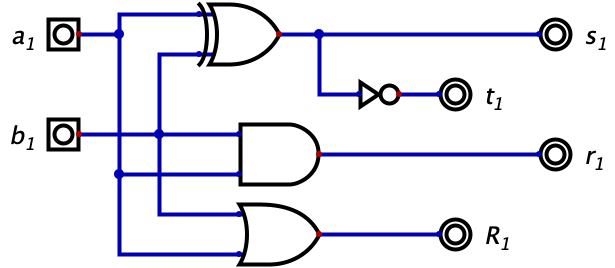
\includegraphics[width=0.45\textwidth]{assets/1bit_adder.png}
\caption{Implementation of a 1-bit Adder with four values output}
\label{fig:1bit_adder}
\end{figure}

To add two 2-bit binary numbers, we first calculate the four values of each corresponding bit. We name them $r_{1,0}, s_{1,0}, R_{1,0}, t_{1,0}$ and $r_{1,1}, s_{1,1}, R_{1,1}, t_{1,1}$ accordingly.
Thus, a 2-bit adder is:
\begin{equation}
    \overline{a_1 a_0} + \overline{b_1 b_0} = \overline{r_1 s_1 s_0} \quad \text{with} \quad \begin{cases}
        r_1 = r_{1,1} \vee (r_{1,0} \wedge R_{1,1}) \\
        s_1 = \begin{cases}
        s_{1,1} \; \text{if} \; r_{1,0} = 0 \\
        t_{1,1} \; \text{if} \; r_{1,0} = 1
        \end{cases} \\
        s_0 \; \text{unchanged}
    \end{cases}
\end{equation}

Similarly, using the notation $1 + \overline{r_1 s_1 s_0} = \overline{R_1 t_1 t_0}$, the 2-bit Adder should calculate the value of $R_1$, $t_1$ and $t_0$ with expressions:

\begin{equation}
    1 + \overline{r_1 s_1 s_0} = \overline{R_1 t_1 t_0} \quad \text{with} \quad \begin{cases}
    R_1 = r_{1,1} \vee (R_{1,1} \wedge R_{1,0}) \\ 
    t_1 = \begin{cases}
        s_{1,1} \; \text{if} \; R_{1,0} = 0 \\
        t_{1,1} \; \text{if} \; R_{1,0} = 1 
    \end{cases} \\
    t_0 \; \text{unchanged}
    \end{cases}
\end{equation}



\begin{figure}[h!]
\centering
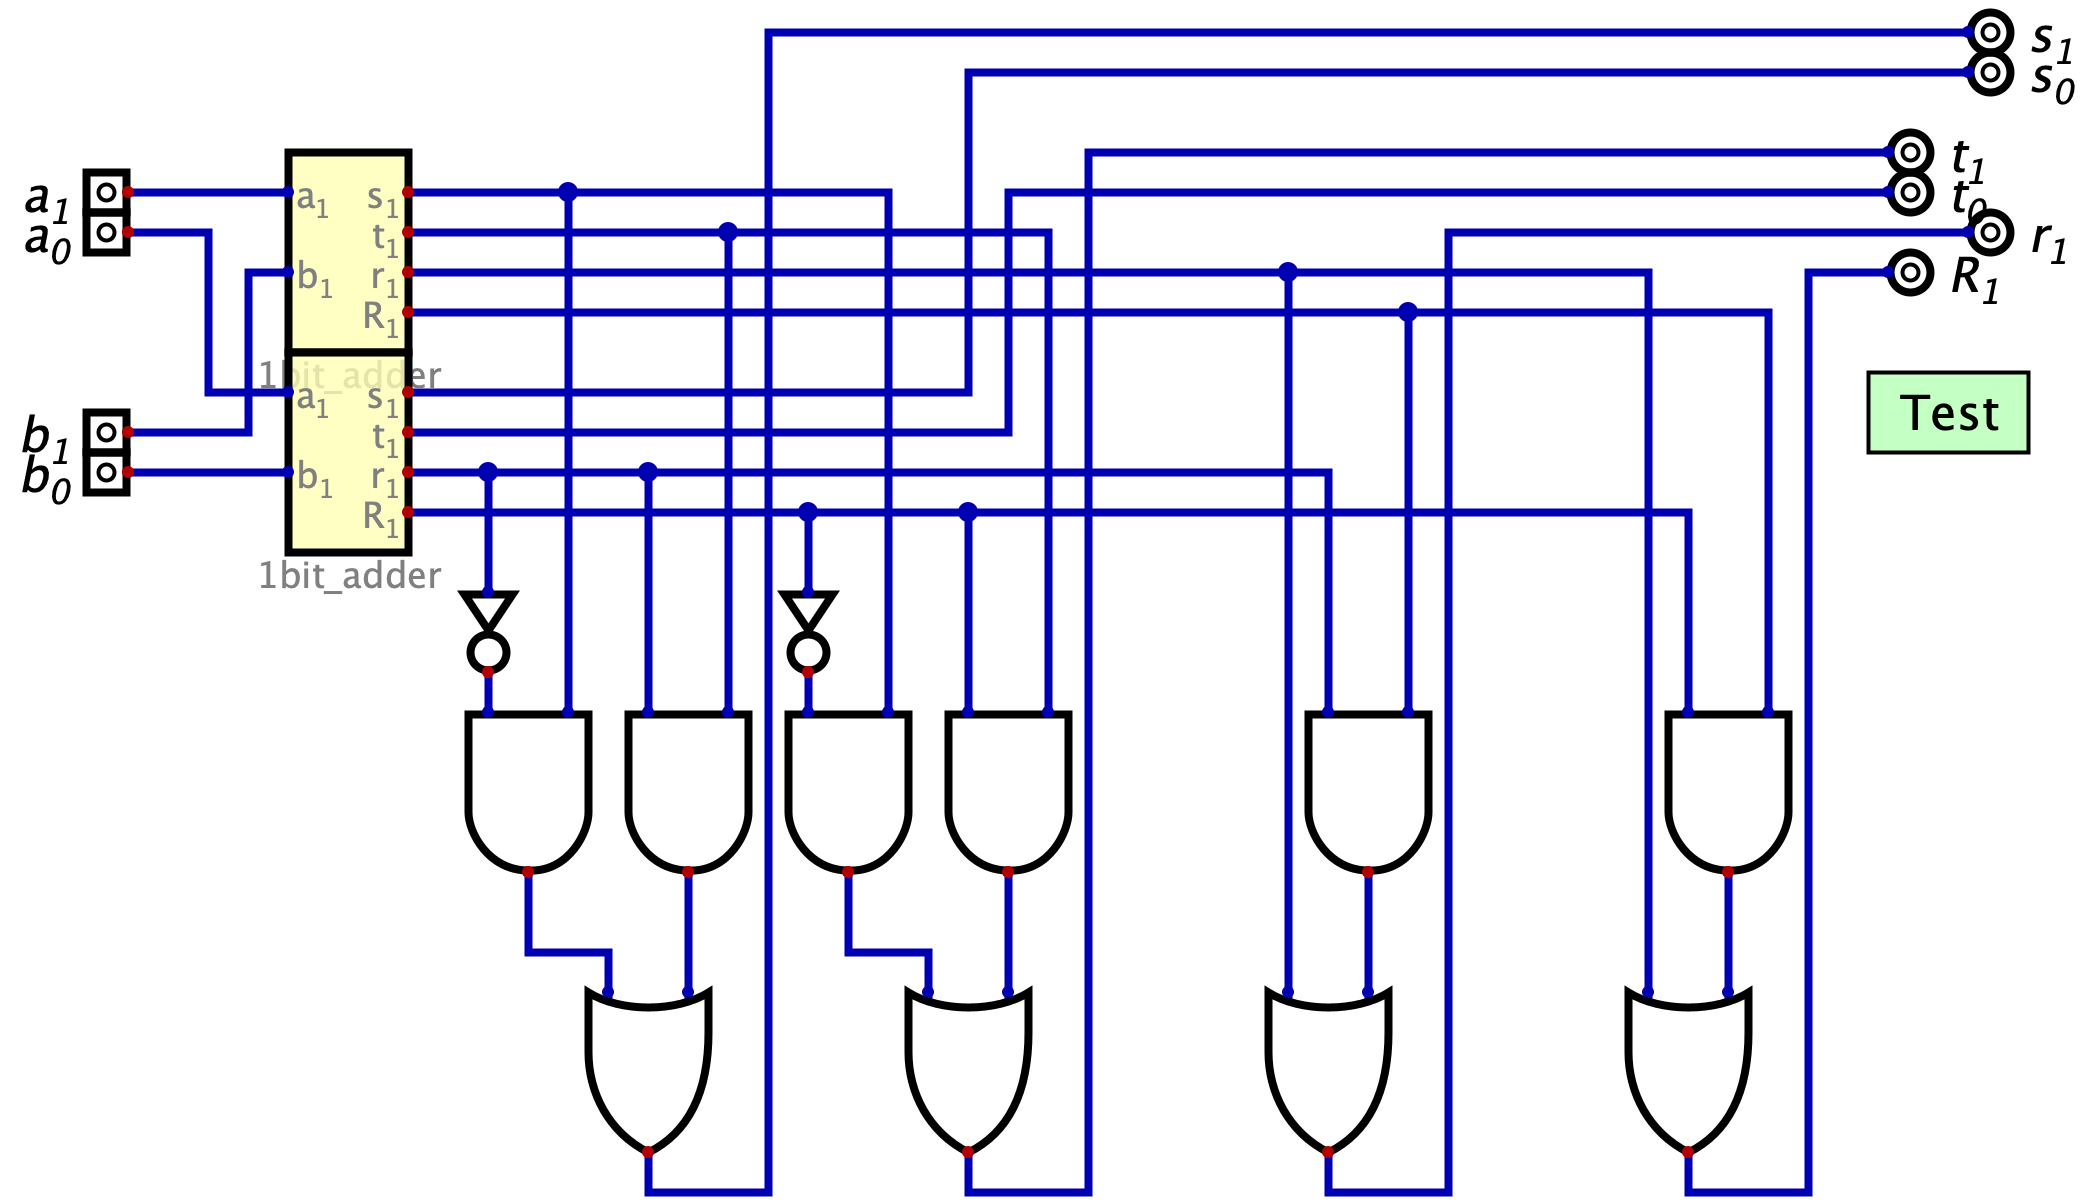
\includegraphics[width=0.45\textwidth]{assets/2bits_adder.png}
\caption{Implementation of a 2-bit Adder with six values output. The 1-bit Adder displayed in Figure~\ref{fig:1bit_adder} is utilized.}
\label{fig:2bits_adder}
\end{figure}

Corresponding circuit implementation is shown in Figure~\ref{fig:2bits_adder}.


In general, to add between $2^p$-bit binary numbers where $p \in \mathbb{N}^*$ and $p \geq 1$, suppose that the calculation of two $2^{p-1}$-bit Adders are resp. $r_{1,0}, s_{2^{p-1},0}, \dots, s_{1,0}, t_{2^{p-1},0}, \dots, t_{1,0}, R_{1,0}$ and $r_{1,1}, s_{2^{p-1},1}, \dots, s_{1,1}, t_{2^{p-1},1}, \dots, t_{1,1}, R_{1,1}$, depending on values of $r_{1,0}$ and $R_{1,0}$:
\begin{itemize}
    \item If $r_{1,0}=0$ and $R_{1,0}=0$, $r_1 = r_{1,1}$, $R_1 = r_{1,1}$,
    \begin{equation}
        s_k = \begin{cases}
            s_{k,1} \quad \text{if} \quad 1 \leq k \leq 2^{p-1} \\
            s_{k,2} \quad \text{others}
        \end{cases}
    \end{equation}
    and
    \begin{equation}
        t_k = \begin{cases}
            t_{k,1} \quad \text{if} \quad 1 \leq k \leq 2^{p-1} \\
            s_{k,2} \quad \text{others}
        \end{cases}
    \end{equation}
    (Note: the higher half of the $t$ values is equal to $s$ since nothing would be changed even if the binary number is added by one)
    \item If $r_{1,0}=0$ and $R_{1,0}=1$, we concatenate the result, that is to say, $r_1 = r_{1,1}$, $R_1 = R_{1,1}$,
    \begin{equation}
        s_k = \begin{cases}
            s_{k,1} \quad \text{if} \quad 1 \leq k \leq 2^{p-1} \\
            s_{k,2} \quad \text{others}
        \end{cases}
    \end{equation}
    and
    \begin{equation}
        t_k = \begin{cases}
            t_{k,1} \quad \text{if} \quad 1 \leq k \leq 2^{p-1} \\
            t_{k,2} \quad \text{others}
        \end{cases}
    \end{equation} 
    \item If $r_{1,0}=1$ and $R_{1,0}=1$, we concatenate the result, that is to say, $r_1 = R_{1,1}$, $R_1 = R_{1,1}$,
    \begin{equation}
        s_k = \begin{cases}
            s_{k,1} \quad \text{if} \quad 1 \leq k \leq 2^{p-1} \\
            t_{k,2} \quad \text{others}
        \end{cases}
    \end{equation}
    and
    \begin{equation}
        t_k = \begin{cases}
            t_{k,1} \quad \text{if} \quad 1 \leq k \leq 2^{p-1} \\
            t_{k,2} \quad \text{others}
        \end{cases}
    \end{equation} 
\end{itemize}

Based on this analysis, a 4-bit Adder with ten values output is shown in Figure~\ref{fig:4bits_adder}, and an 8-bit Adder with eighteen values output is shown in Figure~\ref{fig:8bits_adder}.


\begin{figure}[h!]
\centering
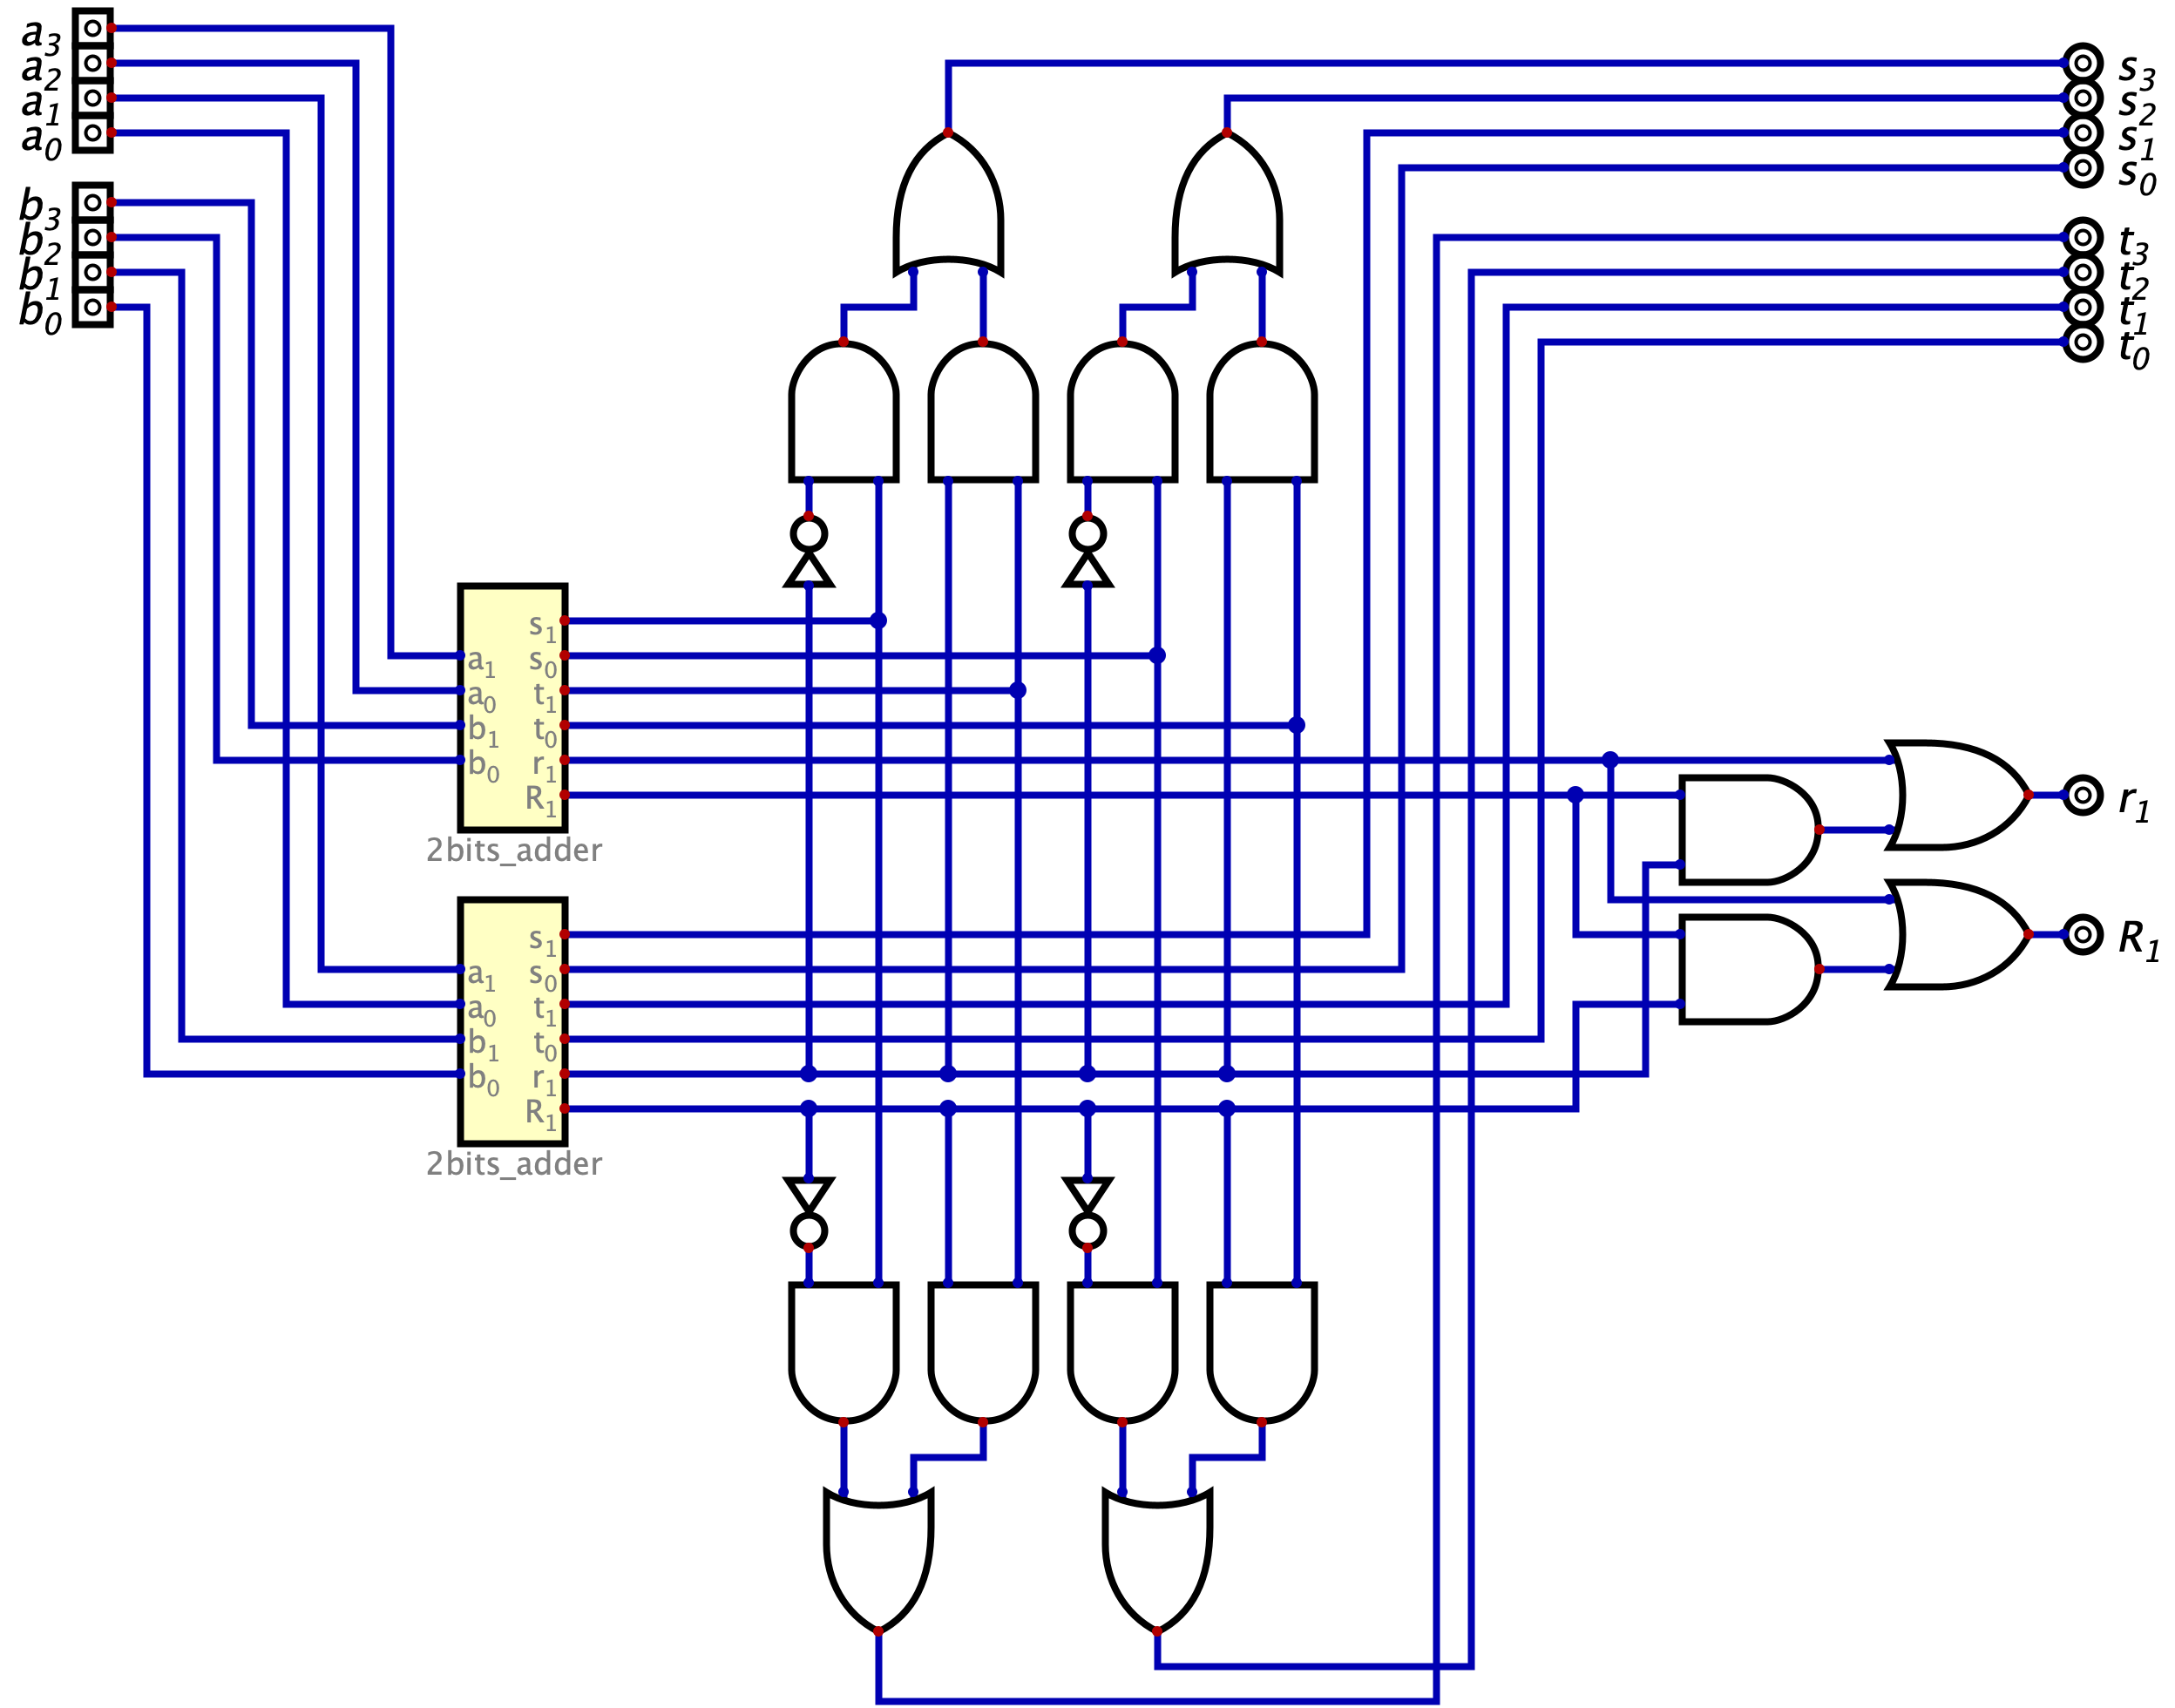
\includegraphics[width=0.45\textwidth]{assets/4bits_adder.png}
\caption{Implementation of a 4-bit Adder with eight values output. The 2-bit Adder displayed in Figure~\ref{fig:2bits_adder} is utilized.}
\label{fig:4bits_adder}
\end{figure}

\begin{figure}[h!]
\centering
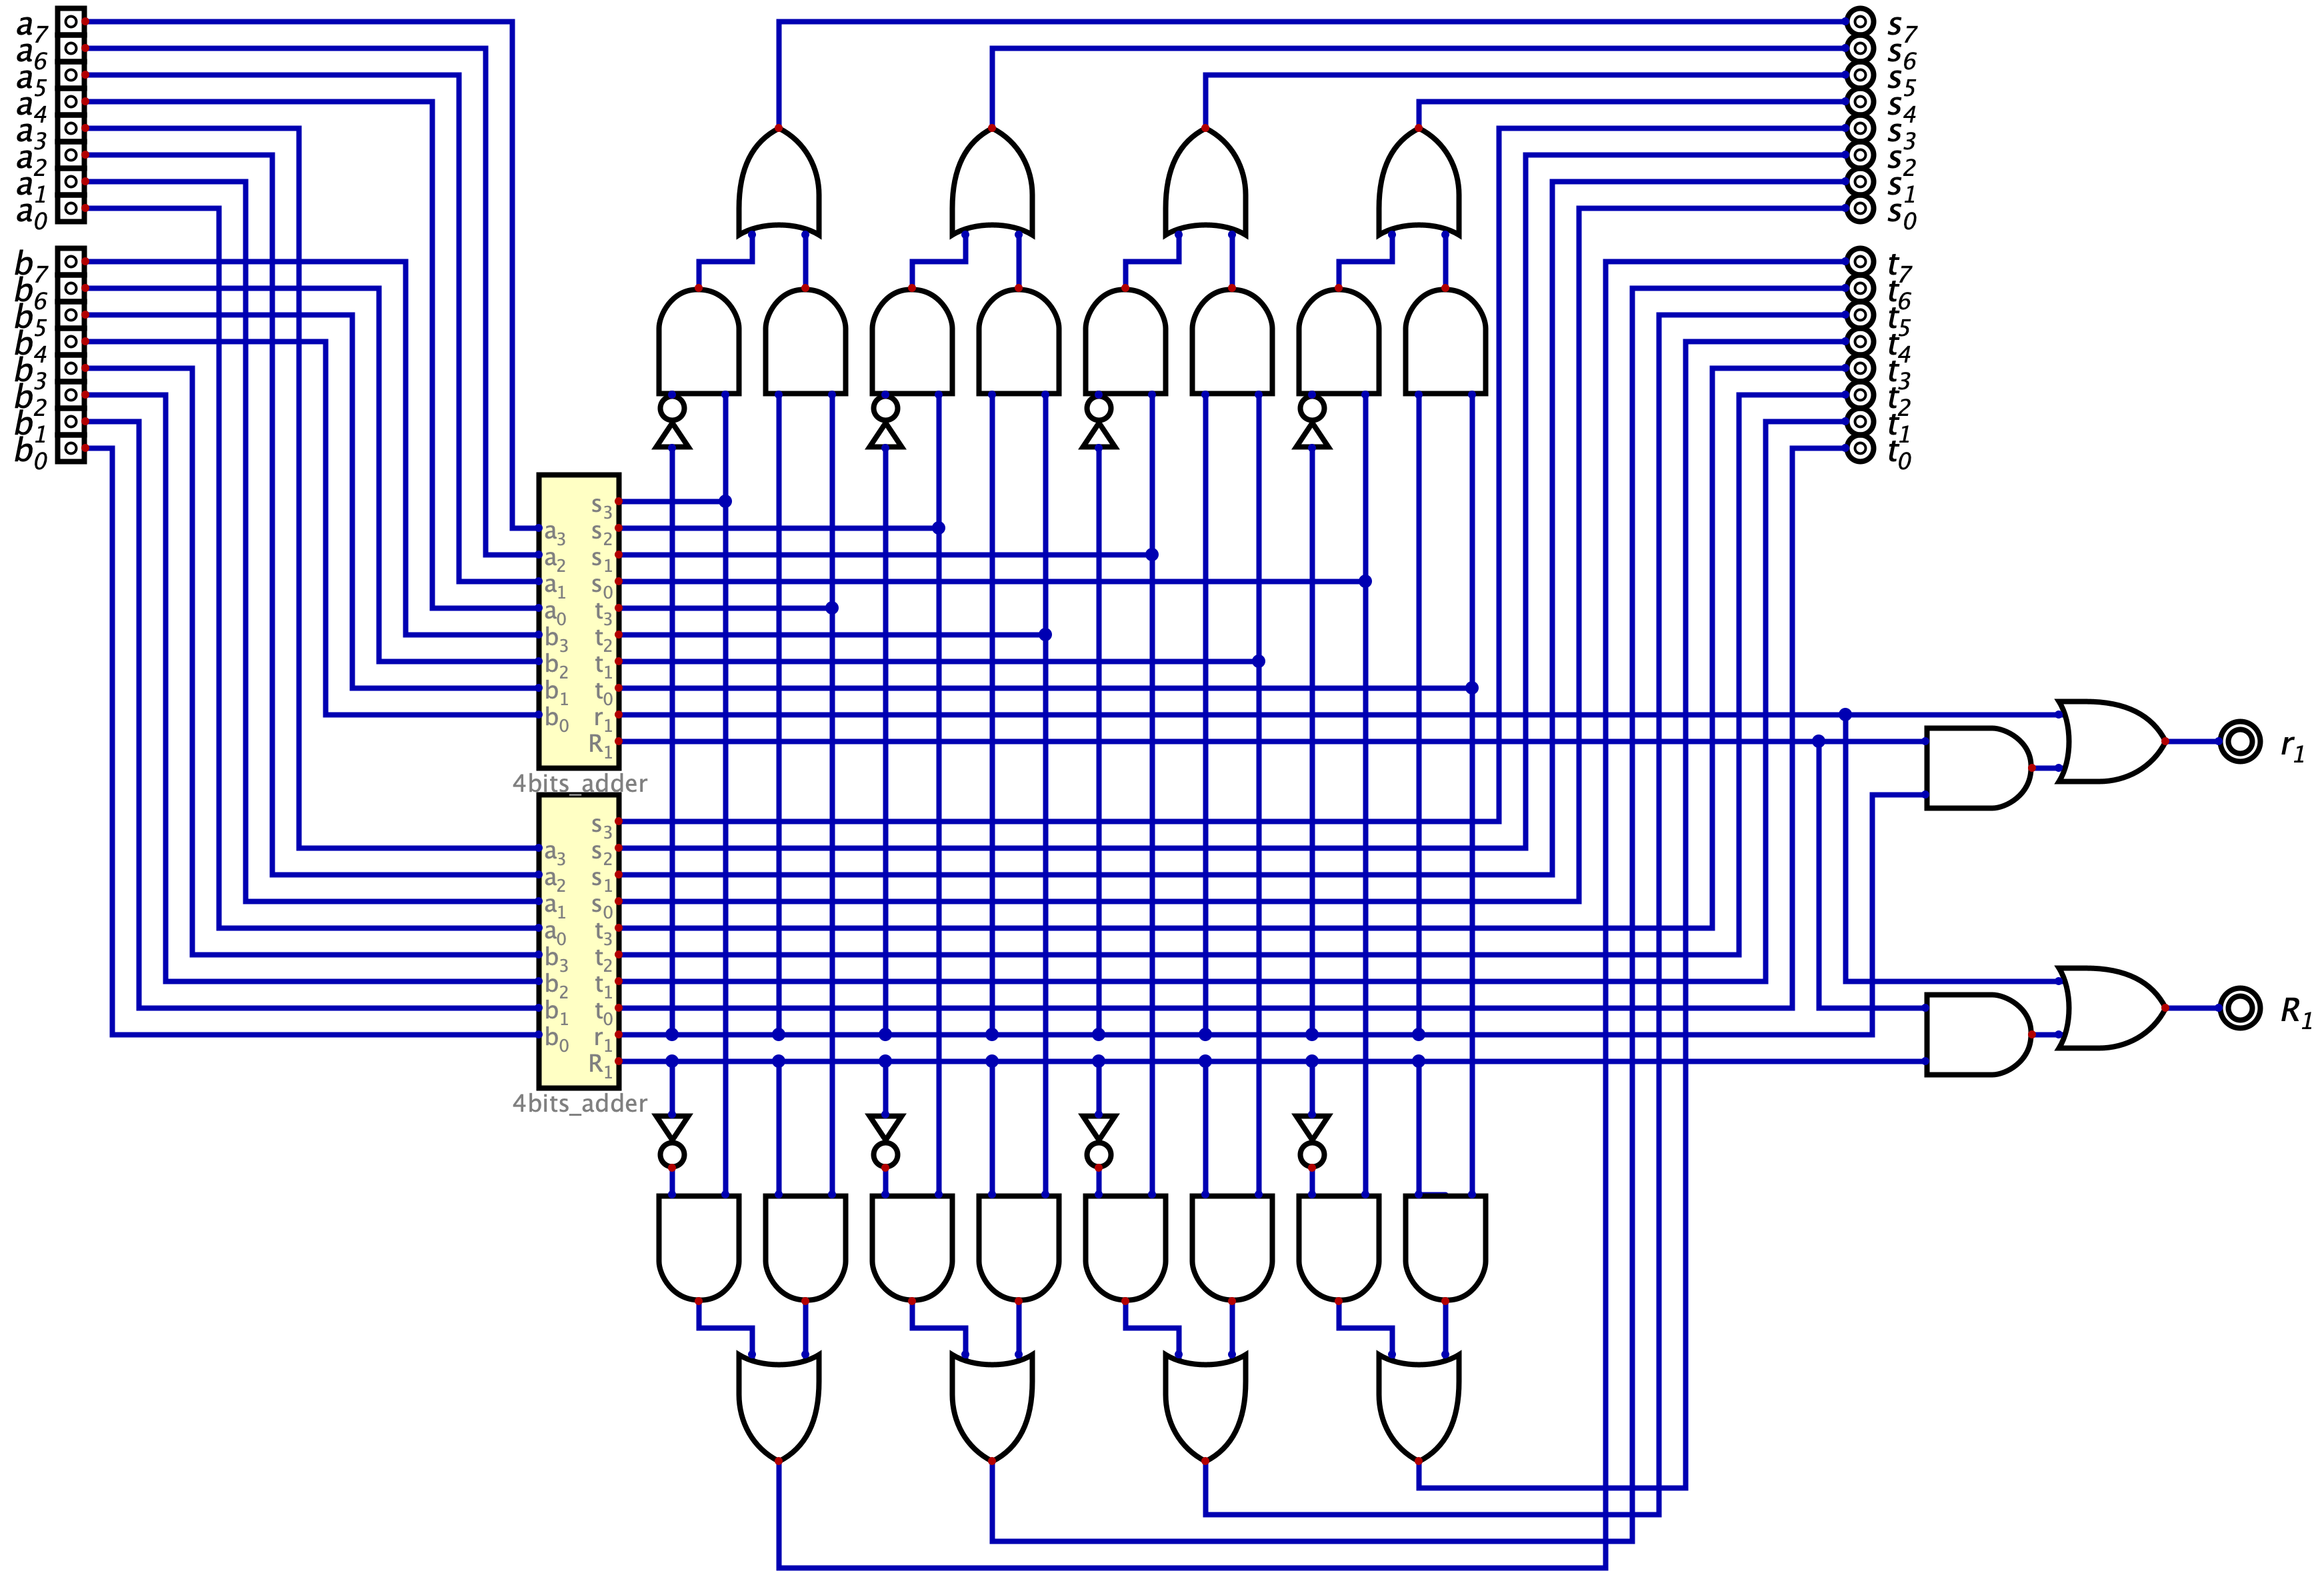
\includegraphics[width=0.45\textwidth]{assets/8bits_adder.png}
\caption{Implementation of an 8-bits Adder with eighteen values output. The 4-bit Adder displayed in Figure~\ref{fig:4bits_adder} is utilized.}
\label{fig:8bits_adder}
\end{figure}

Using the 8-bit Adder implemented above, we design our final edition of the two's complement circuit: Using Multiplexer, the circuit is displayed in Figure~\ref{fig:twos_complement_course}.


\begin{figure}[h!]
\centering
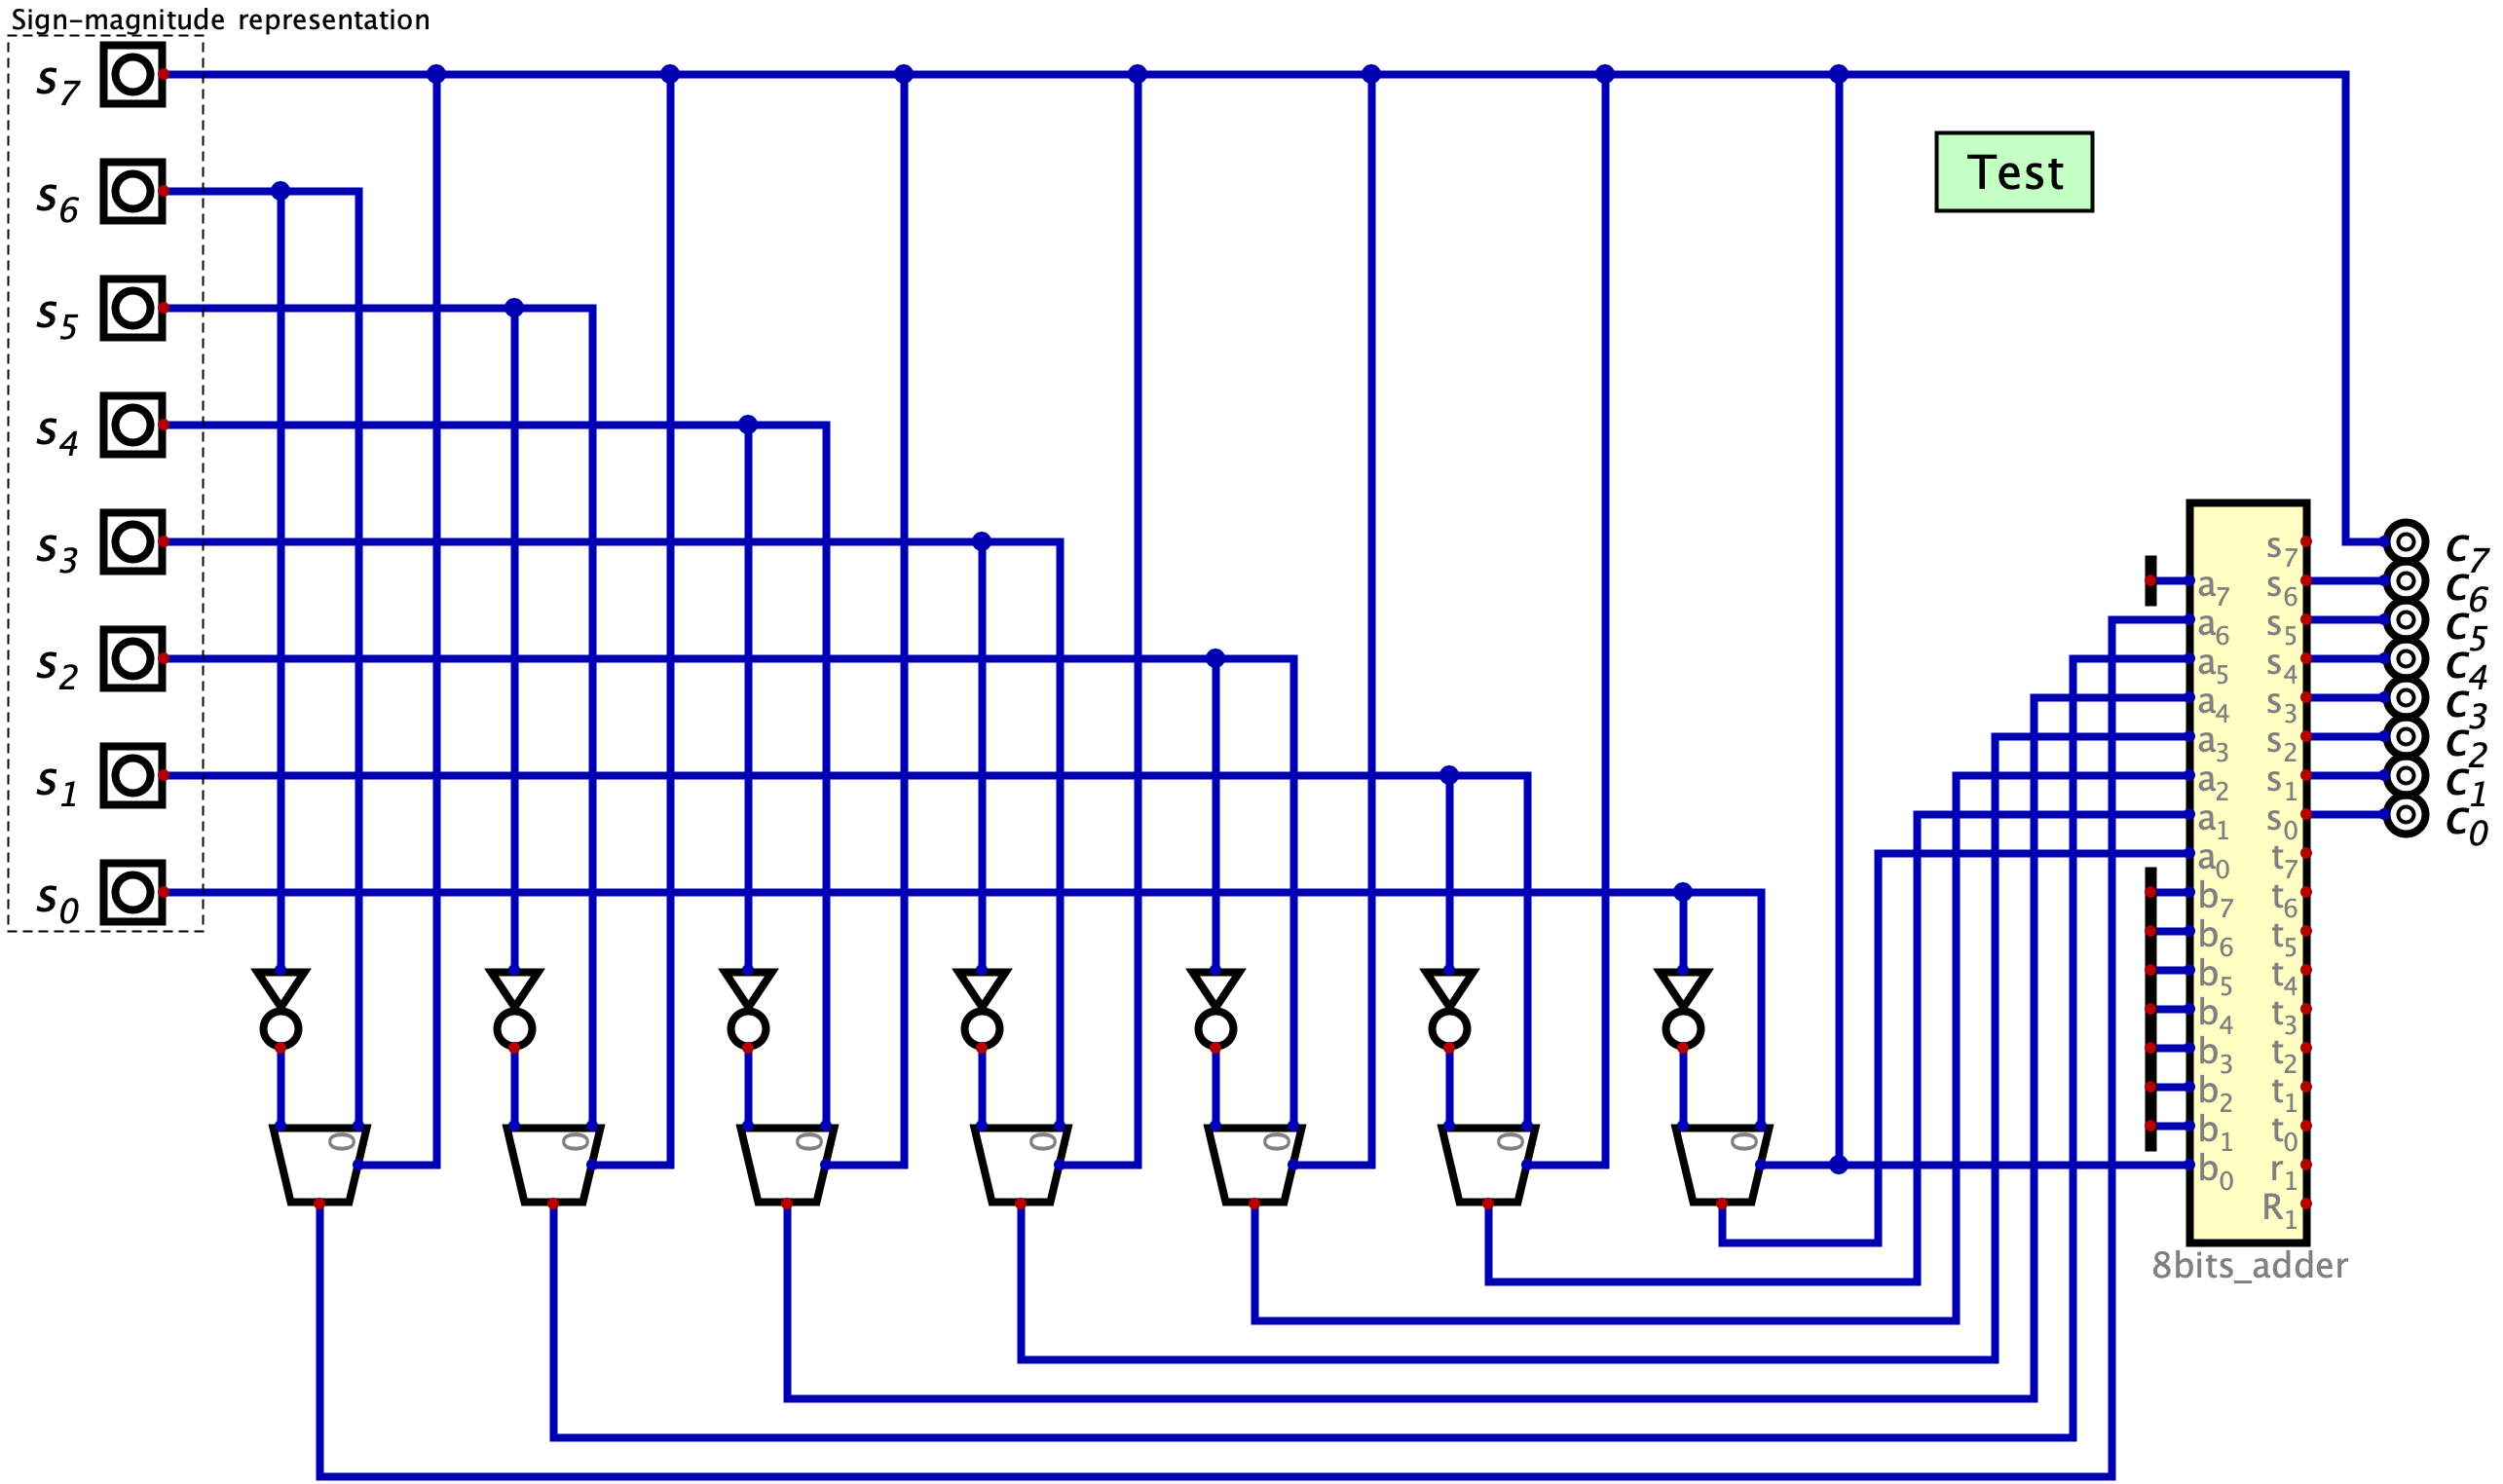
\includegraphics[width=0.45\textwidth]{assets/twos_complement_course.png}
\caption{Implementation of an 8-bits Two's Complement Circuit with Divide and Conquer Method. The 8-bit Adder displayed in Figure~\ref{fig:8bits_adder} is utilized.}
\label{fig:twos_complement_course}
\end{figure}


    
\subsection{Question 4}

\subsubsection{Calculation for the first implementation}\label{sec:q4}


For an 8-bit two's complement circuit implemented in Section~\ref{sec:3-A}, to calculate the depth and complexity of the circuit, we divide the circuit into two parts:
\begin{enumerate}
    \item In the \textbf{inversion stage}, all components are inverted simultaneously, thus depth is 1 and the number of NOT gates required is 7.
    \item In the \textbf{addition stage}, the two 4-bit lookahead carry adders are connected in series.
          For a single 4-bit lookahead adder, its depth is 2 since one for the AND gates and one for the Half-Adders. The number of gates utilized is:
          \begin{equation}
            4 + 4 \times 2 = 12
          \end{equation}
          Since there are two lookahead carry adders, therefore, its depth is 4 and its complexity is 24.

\end{enumerate}

Therefore, for an 8-bit circuit, its depth is $1+4=5$ and its complexity is $7+24=31$.

Now, for any $2^p$-bit two's complement circuit, the inversion stage is unchanged: the depth is 1 and the complexity is $2^p-1$ in this stage. We need to count how many 4-bit Lookahead adders are needed.

The main concept is to divide the large binary number into groups of 4-bit binary numbers. After that, we put them into series. The number of groups: 
\begin{equation}
    \begin{cases}
        \frac{2^p}{4} = 2^{p-2} \quad &\text{if} \quad p \geq 2     \\
        1 &\text{if} \quad  p = 0, \; 1
    \end{cases}
\end{equation}

Therefore, The depth is $2\times 2^{p-2} = 2 ^{p-1}$ and the complexity is $12 \times 2^{p-2} = 3 \times 2^p$ in the addition stage.


\textbf{Conclusion: For $p \geq 1$, the depth is $2^{p-1} + 1$ and the complexity is $2^p - 1 + 3 \times 2^p = 2^{p+2}-1$}.


\subsubsection{Calculation for the second implementation}\label{sec:q4-2}

For the circuit implemented in Section~\ref{sec:3-B}, the depth could be calculated as follows:

\begin{itemize}
    \item In the \textbf{inversion stage}, the depth is 1 and the number of NOT gates required is 7.
    \item In the \textbf{addition stage}, suppose that to implement a $2^{p-1}$-bit adder where $p \in \mathbb{N}^*$ and $p \geq 1$, the depth in this stage (Note: it is worthy to limit the range only in the addition stage) is $d_{p-1}$ and the complexity is $c_{p-1}$. 
    Therefore, the depth of a $2^p$-bit adder in this stage is 
    \begin{equation}
        d_p = d_{p-1} + 3
    \end{equation}
    since the longest route is NOT gate-AND gate-OR gate.
    Moreover, the complexity in this stage is
    \begin{equation}\label{eq:complexity}
        c_p = 2 \times c_{p-1} + 4 \times 2^p + 2 \times 2
    \end{equation}
\end{itemize}

We then calculate the expression for $d_p$ and $c_p$ based on their recurrent expressions.

\begin{equation}
    d_p = \begin{cases}
        2 \quad &\text{if} \quad p = 0 \\
        3p + d_0 = 3p + 2 &\text{others}
    \end{cases}
\end{equation}

The solution for the homogeneous part of Equation~\ref{eq:complexity} is $c_p^{(h)} = A \times 2^p$. Suppose the particular solution $c_p^{(p)} = k_p\times 2^p$ where the expression of $k_p$ to be determined.

\begin{gather*}
    k_p \times 2^p = 2 \times k_{p-1} \times 2^{p-1} + 4 \times (2^p+1) \\
    k_p - k_{p-1} =4 + 4 \times \frac{1}{2^p}
\end{gather*}

Therefore the expression of $k_p$ is 

\begin{equation}
    k_p = k_0 +  4p + 4 \times \sum_{i=1}^{p} \frac{1}{2^i} = k_0 + 4p+4- \frac{4}{2^p}
\end{equation}

Finally, from Figure~\ref{fig:1bit_adder}, $c_0 = 4$ therefore

\begin{equation}
    k_0 \times 2^0 = 4
\end{equation}

$k_0 = 4$ thus the expression of $c_p$ is 

\begin{equation}
    c_p = (8 + 4p - \frac{4}{2^p}) 2^p = (2+ p) \times 2^{p+2} - 4
\end{equation}

We could validate this result by calculating the amount of gates utilized from Figure~\ref{fig:1bit_adder} to \ref{fig:4bits_adder}, where $c_0 = 4$, $c_1=20$, $c_2=60$.


\textbf{Conclusion: Therefore, after considering all of the two stages, as for an 8-bit two's complement circuit, the depth is $3p+3$ and the complexity is $(2+p)2^{p+2} + 3$.}

\subsection{Question 5}

In this section, we use the circuit of Figure~\ref{fig:tc-dq-optimize}.

(Explanation: Since we provide multiple solutions in our project, we consider selecting one of them as feasible since it is not specified in the question. To export the circuit of Figure~\ref{fig:twos_complement} needs to change all
the output labels $R_1$ into some other alphabets, as we have tested that it would lead to errors, saying that the name $r$ and $R$ collide with each other.)

We export the VHDL code based on the circuit designed in the Digital software and generate the code using gtkwave.
Reminding that the input 8-bit binary number and the output 8-bit binary number are represented by:
\begin{equation}
    \overline{s_7s_6s_5s_4s_3s_2s_1s_0} \longrightarrow \overline{c_7c_6c_5c_4c_3c_2c_1c_0}
\end{equation}


The text data is listed in Figure~\ref{fig:test-benchmark}.

\begin{figure}[h!]
    \centering
    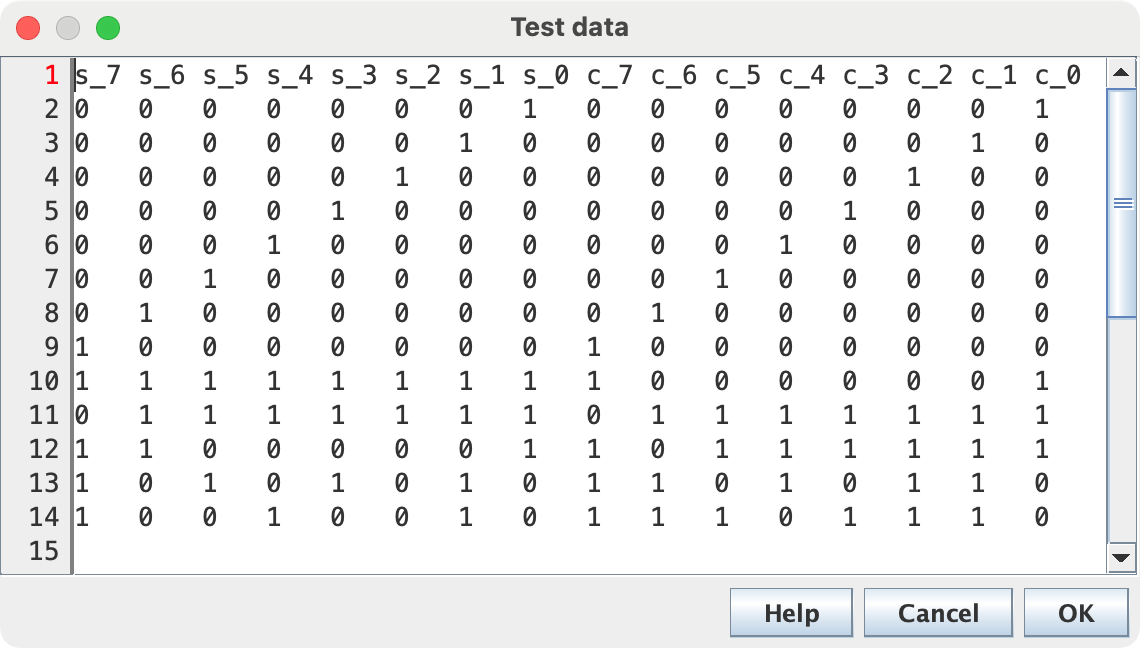
\includegraphics[width=0.5\textwidth]{assets/test-data.png}
    \caption{Test Benchmark}
    \label{fig:test-benchmark}
\end{figure}


As is required, all the ports/input-output have a delay of 1 unit time and all the multiplexer have a delay of 2 unit time.
The corresponding simulation of signals is shown in Figure~\ref{fig:result-with-delay}.


Analysis of the result:
\begin{itemize}
    \item Setting the delay of the multiplexer as 2 and the delay of the NOT gate as 1 allows us to directly exploit the result of the NOT gate after the result is calculated. (Figure~\ref{fig:analysis1})
    \item The calculation of the two 4-bit Lookahead Carry Adder proved the fact the two adders are connected in series. One would begin to operate only after the other has finished its calculation. (Figure~\ref{fig:analysis2})
\end{itemize}

(An equivalent expression is shown in Figure~\ref{fig:delay}. It is worthy to note that this code cannot generate VHDL code for the reason that the delay component is not implemented in VHDL (at least not in Digital software))


\begin{figure}[h!]
    \centering
    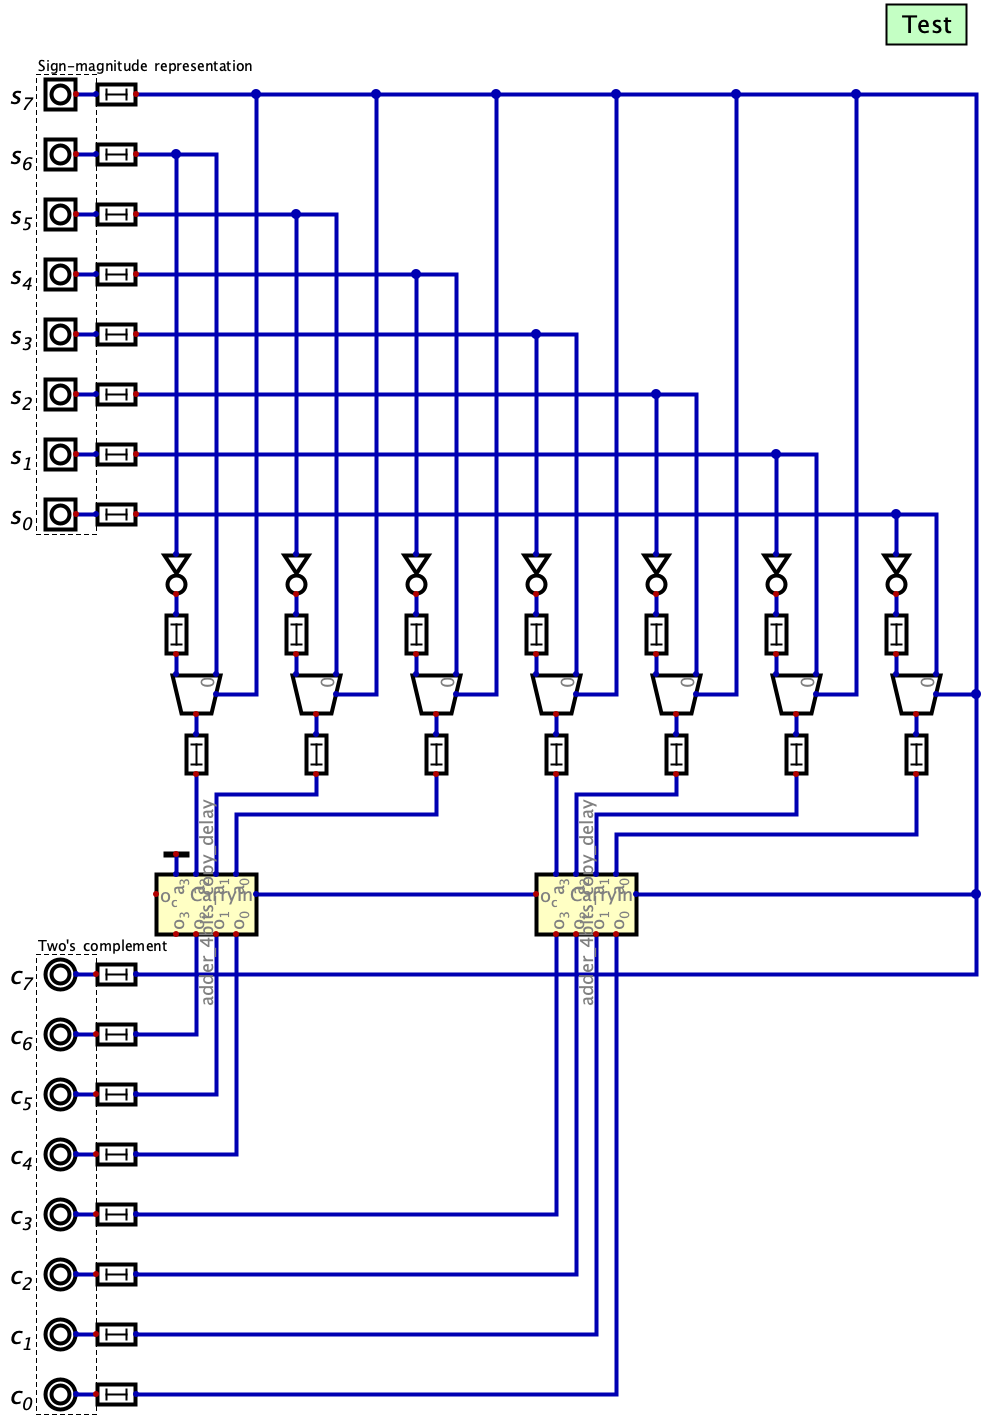
\includegraphics[width=0.5\textwidth]{assets/twos_complement_dq_copy_delay.png}
    \caption{Equivalent Representation of the circuit combined with delayed I/O, Gates and Multiplexers. This Representation is also useful to understand the Analysis 1. Part}
    \label{fig:delay}
\end{figure}


\begin{figure}[h!]
    \centering
    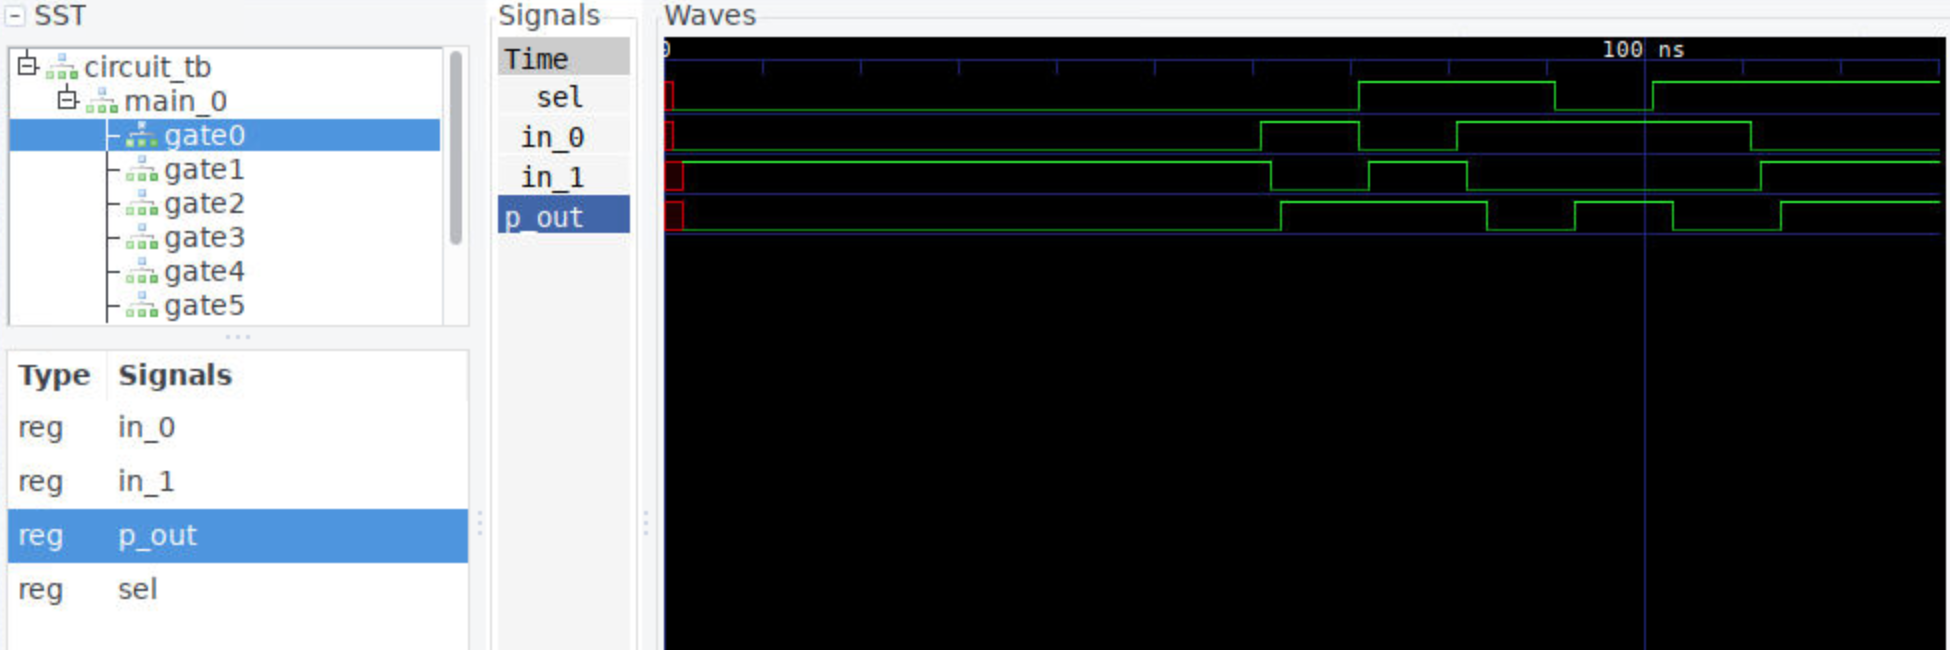
\includegraphics[width=0.5\textwidth]{assets/gtkwave-1.png}
    \caption{Analysis 1: Observation of the time delay of the component {NOT Gate + Multiplexer}. After the signal is passed to the NOT Gate, the NOT Gate generates the result after 1 ns, and the multiplexer generates the result after 2 ns, which is time-efficient}
    \label{fig:analysis1}
\end{figure}

\begin{figure}[h!]
    \centering
    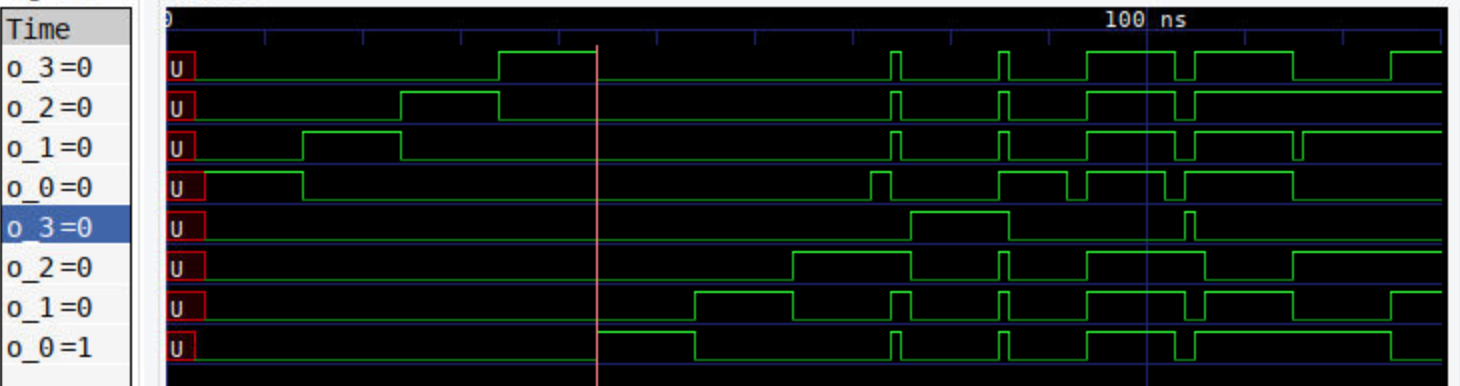
\includegraphics[width=0.5\textwidth]{assets/gtkwave-2.png}
    \caption{Analysis 2: Observation of the time delay of the two 4-bit Lookahead Carry Adders. The upper four signals correspond to the lower 4 bits of the output. (Note that here, $o_3$ has no actual meaning since the highest bit should be the sign bit)}
    \label{fig:analysis2}
\end{figure}

\begin{figure}[h!]
    \centering
    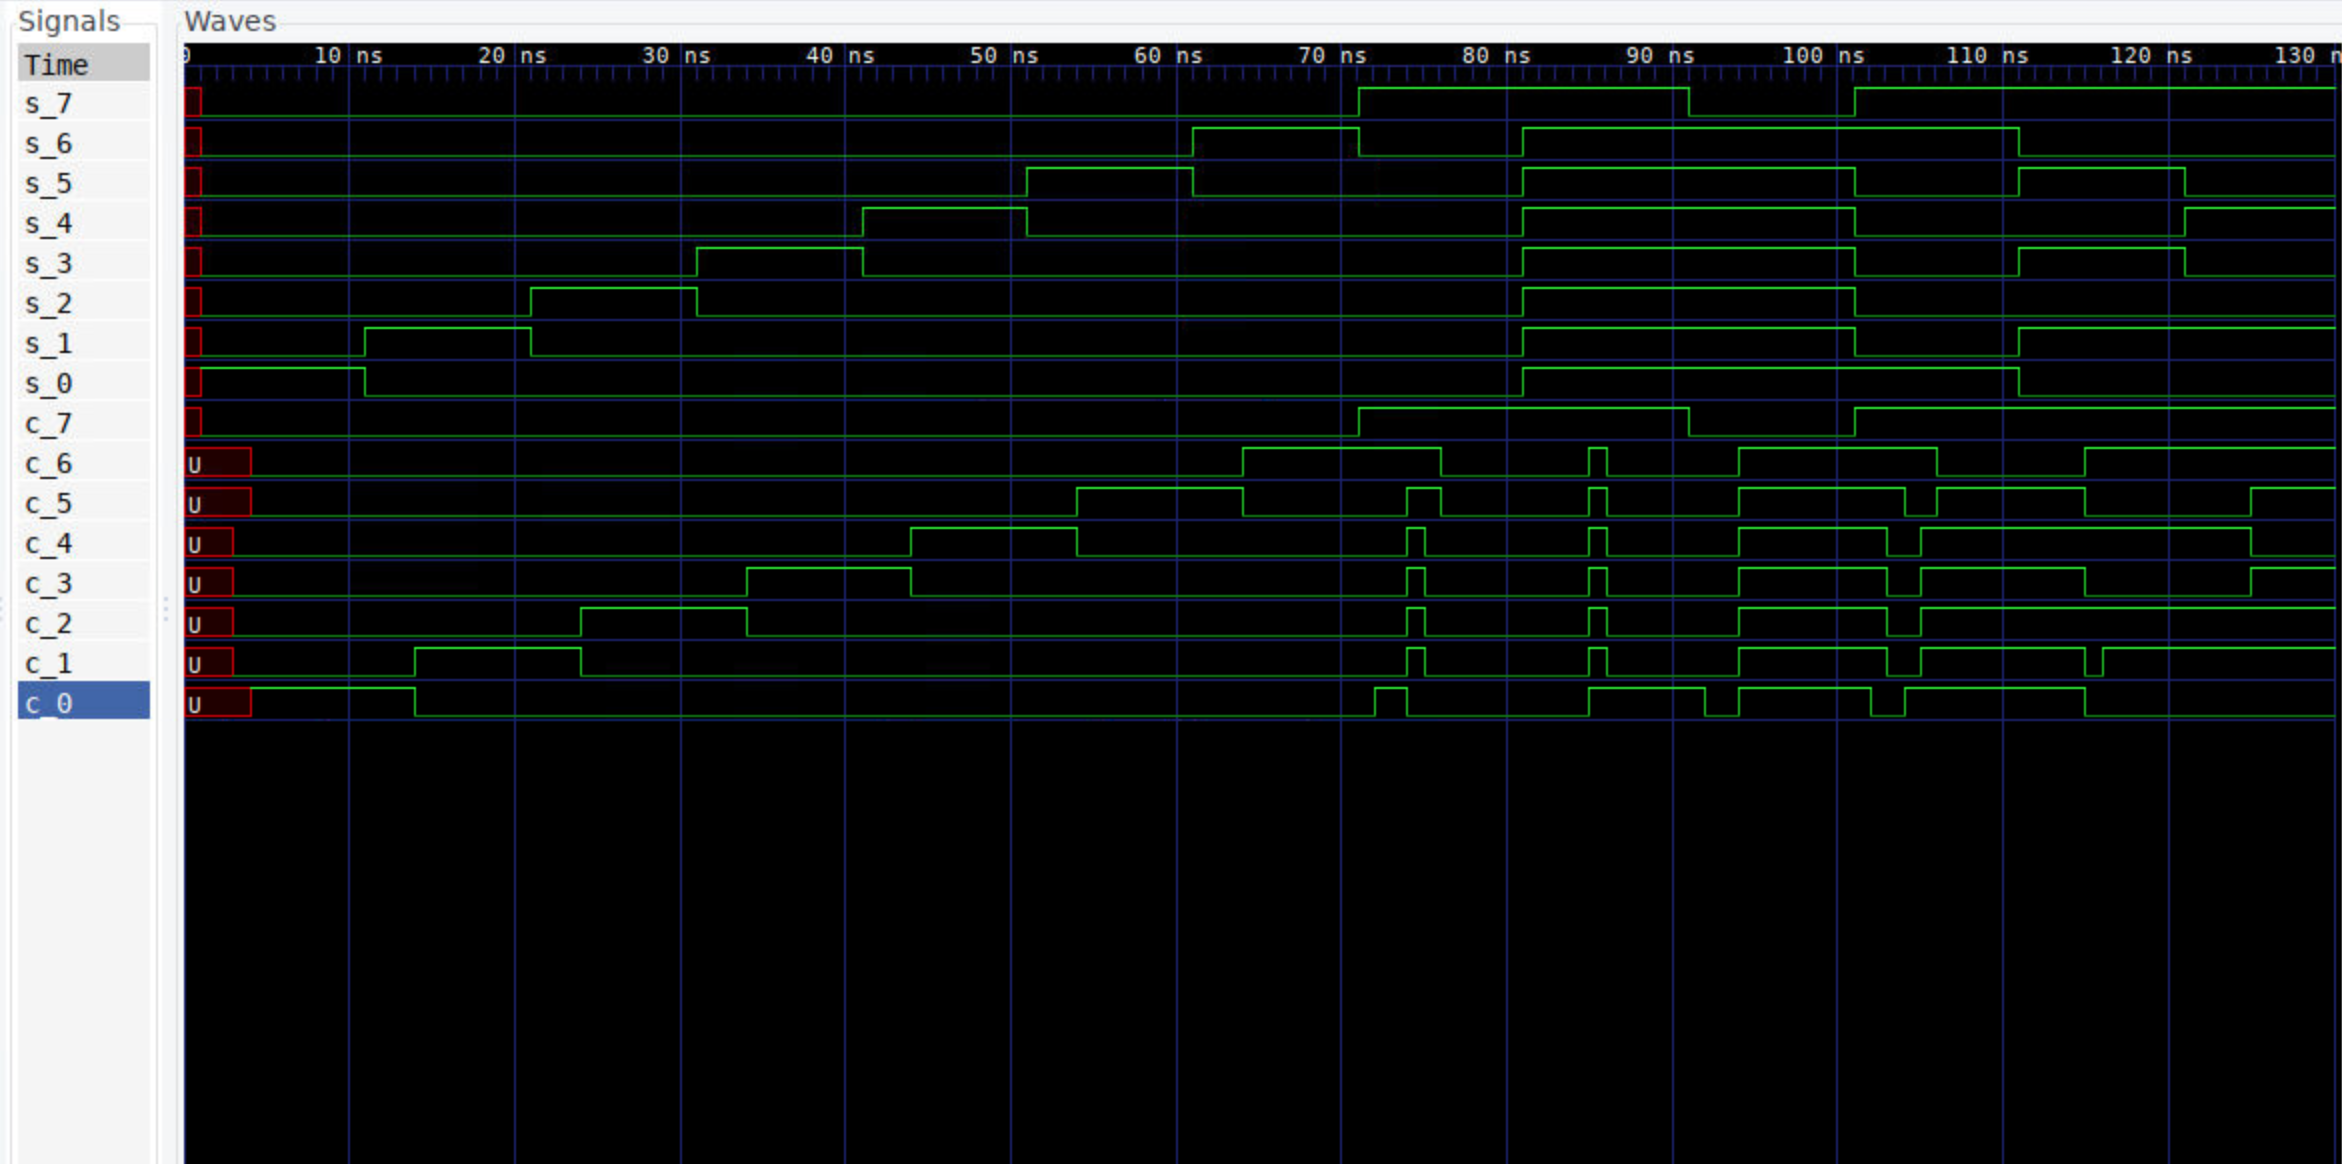
\includegraphics[width=0.5\textwidth]{assets/gtkwave.png}
    \caption{Result with delay with test data in Figure~\ref{fig:test-benchmark}}
    \label{fig:result-with-delay}
\end{figure}

\section{Question 6-10}

\subsection{Question 6}

To execute the operation, it is essential to:
\begin{enumerate}
    \item Fetch the number from the Memory
    \item Load them in the Register
    \item The ALU read the numbers in the Registers, and output
    \item We load the output result in the Memory.
\end{enumerate}

Consequently, with $M_1$, $M_2$, $M_3$ Memories and $R_1$, $R_2$ Registers, the commands are:

LOAD M1, R1, 0    

LOAD M2, R2, 0    

SUB R1, R2, R1    

STORE R1, M3, 0   

\subsection{Question 7}

The question proposed that four instruction should execute in series, which we will note them:
\begin{itemize}
    \item FI: Fetch instruction
    \item PO: Process Operand
    \item EI: Execute Instruction
    \item WO: Write Operand
\end{itemize}

Undoubtly, the substraction command should wait before the binary numbers have been successfully stored into the corresponding Registers.

\begin{figure}[h!]
    \centering
    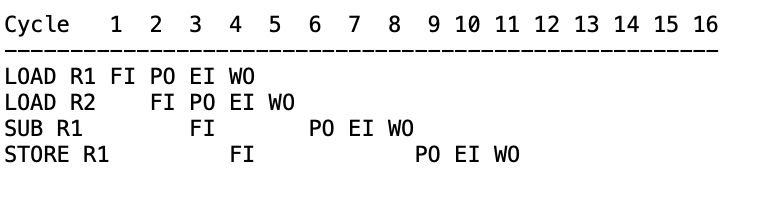
\includegraphics[width=0.5\textwidth]{assets/question-7.png}
    \caption{Pipeline to Execute the Insturctions}
    \label{fig:Question-7}
\end{figure}

\subsection{Question 8}


TBD

\subsection{Question 9}

First, we will introduce several elements embedded in our implementation in the sections later on.


\subsubsection{Trigger}



To synchronize all the signals in the system. We need a clock signal to control all the elements. The term trigger is used to synchronize the signals
with the global status of the whole system. 


In our implementation, an \textbf{impulse signal} is essential so as to enable the operations. For example, it is utile when we wish to execute the read command to a certain Memory block and to isolate it or switch if off in order for saving energy consumption.

Using the property of a D Flip-Flop Trigger, we output 1 and then 0 in series. Detailed implementation could be found in Figure~\ref{fig:impulse-output}.

\begin{figure}[h!]
    \centering
    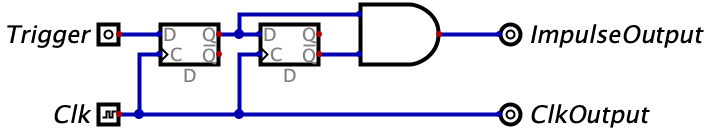
\includegraphics[width=0.5\textwidth]{assets/impulse-output.png}
    \caption{Impulse Signal Trigger}
    \label{fig:impulse-output}
\end{figure}


\subsubsection{Memory}



A real memory should consist of several small blocks of storage, each used to store its own numbers. In our implementation, a large memory contains three smaller memory blocks, each capable of storing an 8-bit number.

We proceed step by step.

An 1-bit Memory is implemented in Figure~\ref{fig:1-bit-memory}. To store a single bit, a D Filp-Flop Trigger is utilized. First of all, this 1-bit Memory should be Selected (the input of Operate input should be 1) to function.
When the Read/Write input is 1, the write mode is initiated, and the input is written into the memory. Correspondingly, when the Read/Write input is 0, the read mode is initiated, and the value stored in the memory is output.
The Operate signal should be an impulse signal (which would be implemented later on) in order to automatically switch off the operation mode of the memory after the operation has been executed.

\begin{figure}[h!]
    \centering
    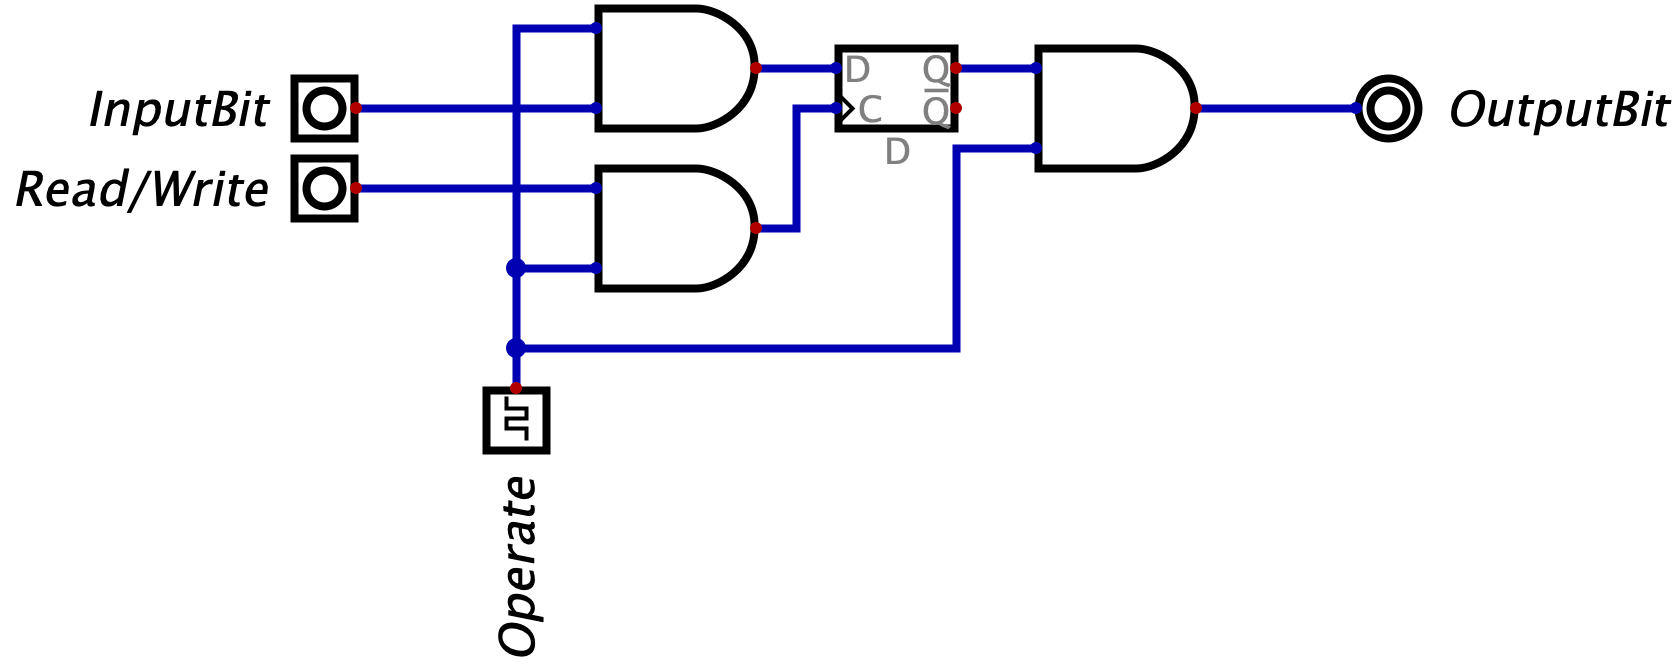
\includegraphics[width=0.5\textwidth]{assets/1-bit-memory.png}
    \caption{Implementation of 1-bit Memory}
    \label{fig:1-bit-memory}
\end{figure}

To store a 8-bits Memory, we parallize the process of storing 8 1-bit binary numbers, which is shown in Figure~\ref{fig:8-bits-memory}.

\begin{figure}[h!]
    \centering
    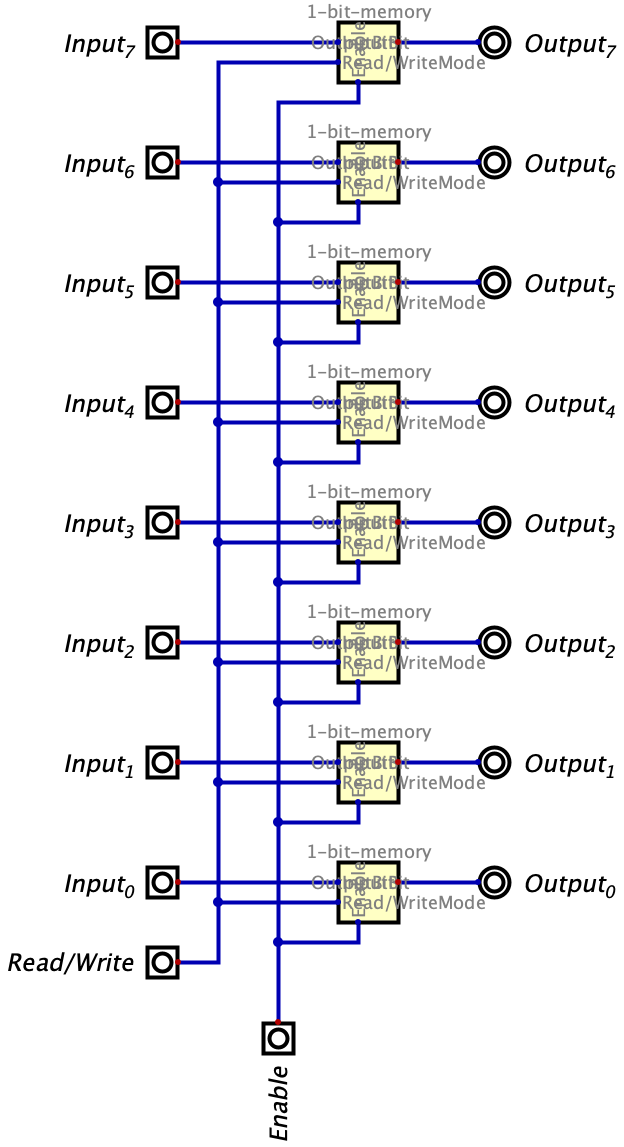
\includegraphics[width=0.4\textwidth]{assets/8-bit-memory.png}
    \caption{Implementation of a single 8-bit Memory Block, the 1-bit Memory shown in Figure~\ref{fig:1-bit-memory} is utilized.}
    \label{fig:8-bits-memory}
\end{figure}

The final structure of the 3-blocks Memory should have a clock cycle signal input to facilitate synchronization when connected to a circuit and to enable sequential execution of instructions. In our implementation, we need the clock to indicate when internal operations are complete. Since the memory contains three smaller memory blocks, the input needs to specify which block should store or retrieve the number.
Traditionally, this should be done by reading the address of the memory block, but we will simplify the process here by directingly reading the indice. After type-in the number to be stored and the memory block to be written in or to be read, when the value of the clock input is 1, it begin to read to the memory block or export the stored value to the output. The implementation is shown in Figure~\ref{fig:8-bits-memories}.

\begin{figure}[h!]
    \centering
    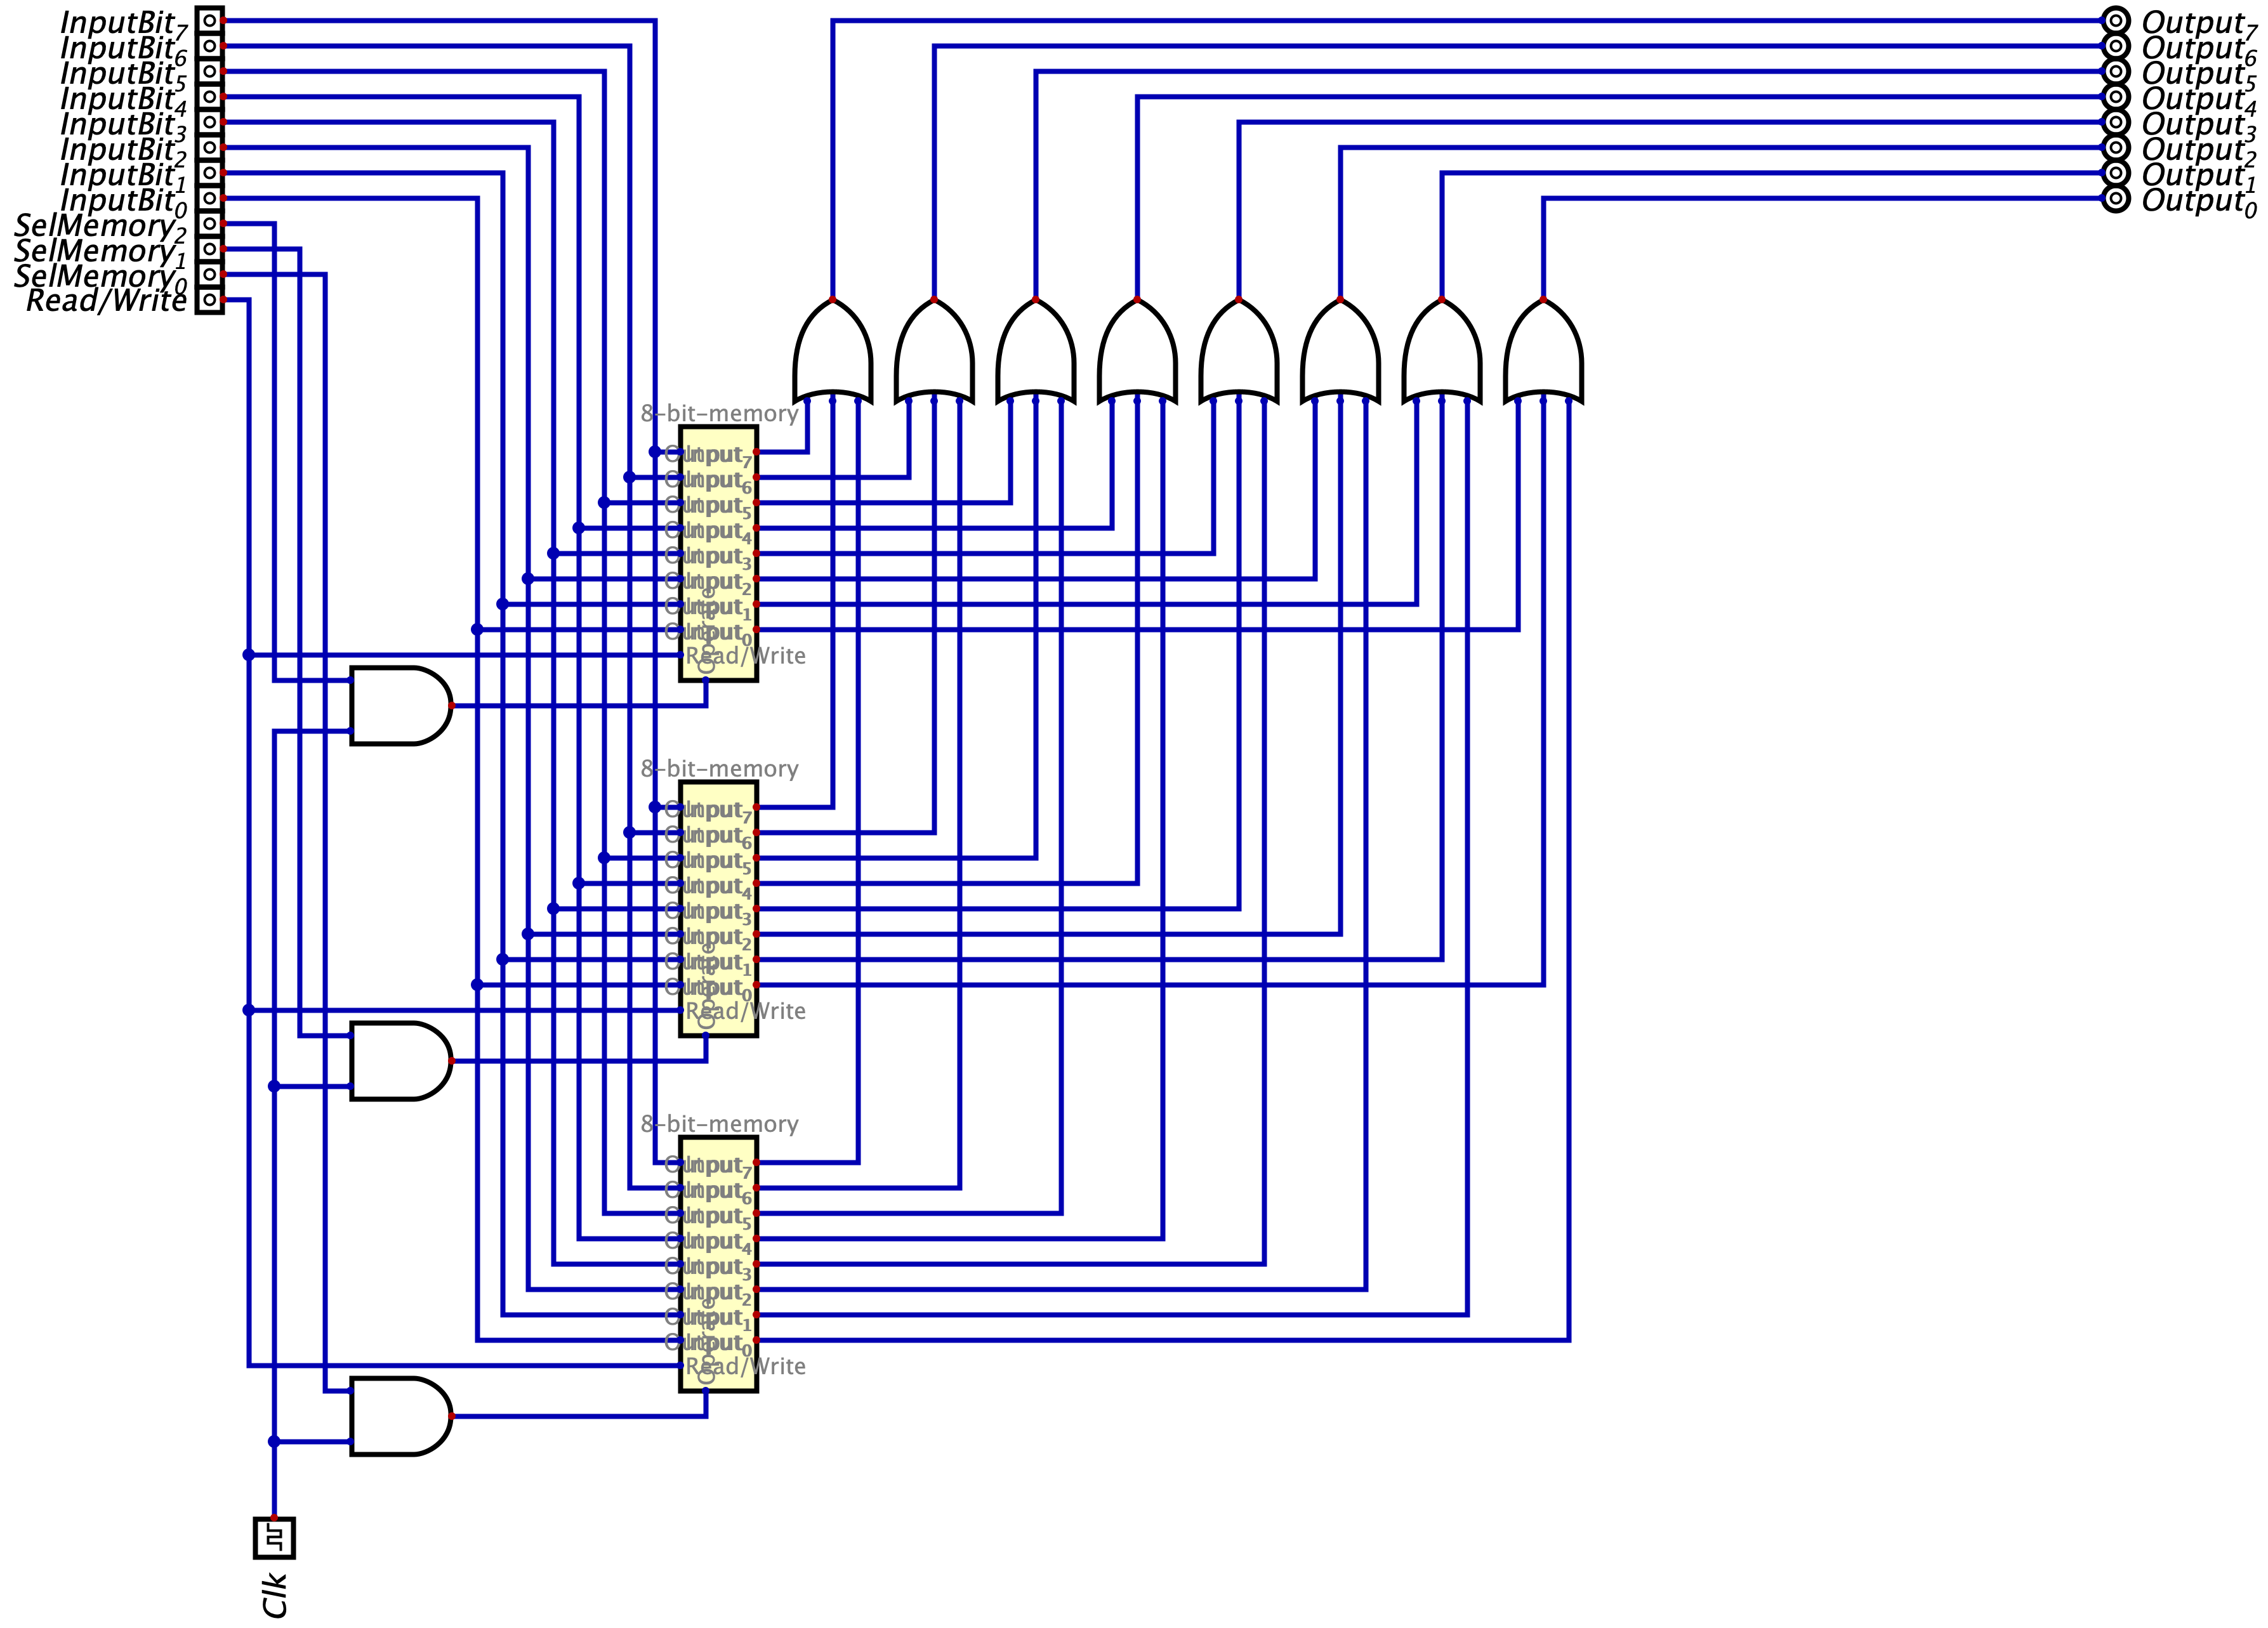
\includegraphics[width=0.5\textwidth]{assets/8-bit-memories.png}
    \caption{Implementation of a 8-bit Memory, three blocks of a 8-bit Memory shown in Figure~\ref{fig:8-bits-memory} is utilized.}
    \label{fig:8-bits-memories}
\end{figure}

\subsubsection{Register}

A 8-bits register is simply bringing together 8 blocks of register, controlled by a clock signal and an enable signal. The register is implemented in Figure~\ref{fig:8-bits-register}.
\begin{figure}[h!]
    \centering
    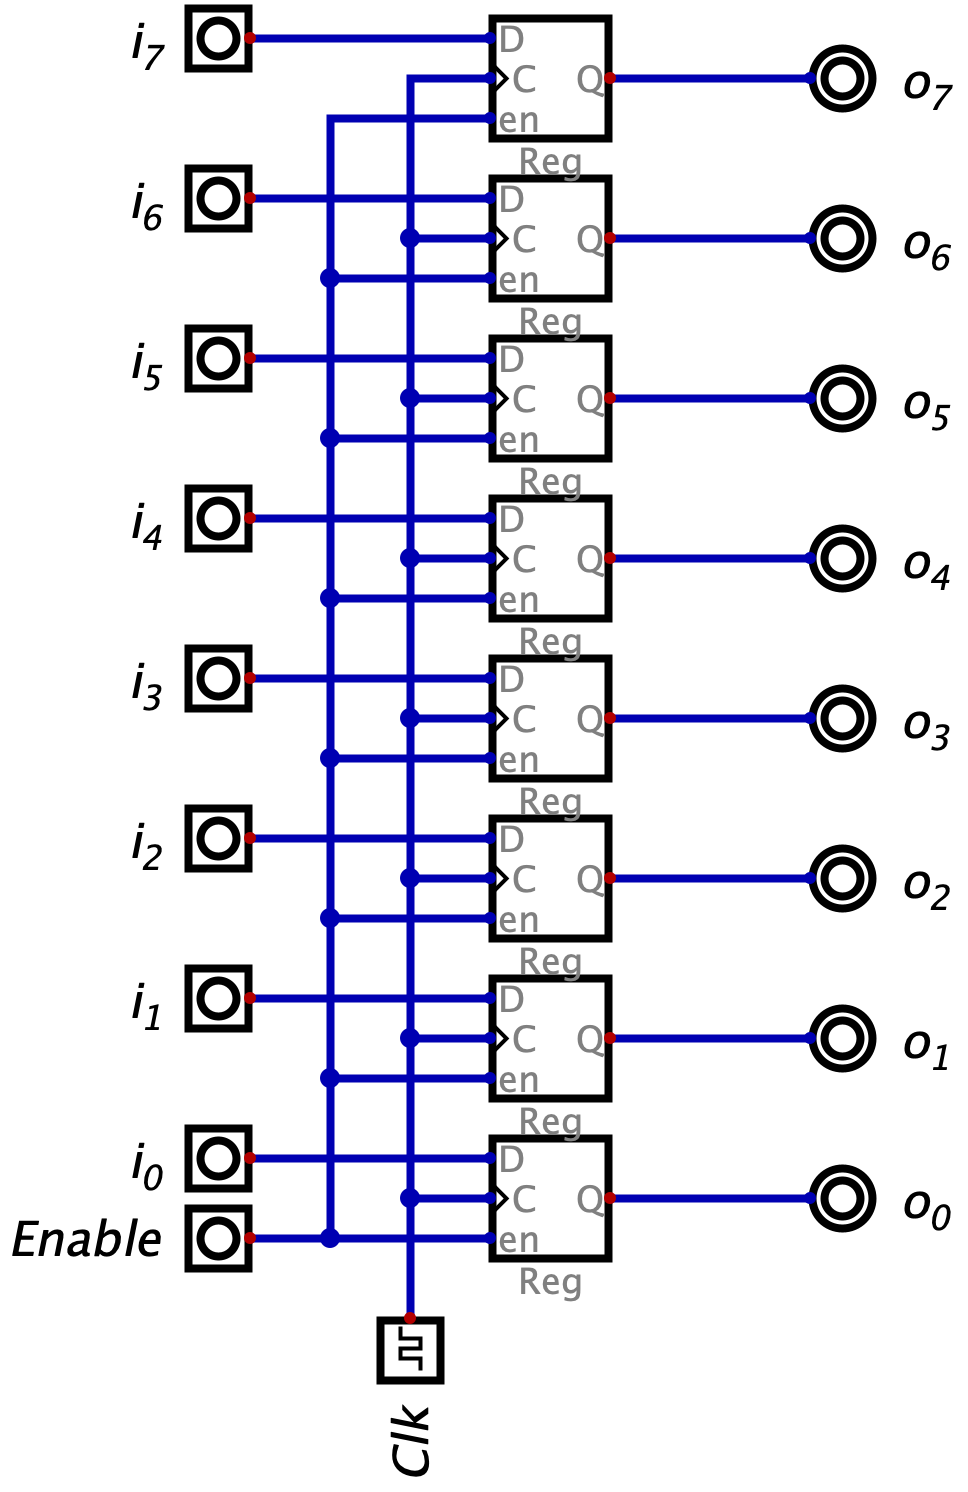
\includegraphics[width=0.3\textwidth]{assets/8-bit-register.png}
    \caption{Implementation of a 8-bits Register.}
    \label{fig:8-bits-register}
\end{figure}


\subsubsection{Store Instruction}
To store some binary numbers, we need the infomation of:
\begin{itemize}
    \item The 8-bit binary number to be input
    \item Which block of the memory should it be stored into
\end{itemize}

We design the circuit by adding an D Filp-Flop Trigger to synchronize the operation with the global clock. The circuit to implement the store instruction for one single memory is shown in Figure~\ref{fig:store_1bit}.

\begin{figure}[h!]
    \centering
    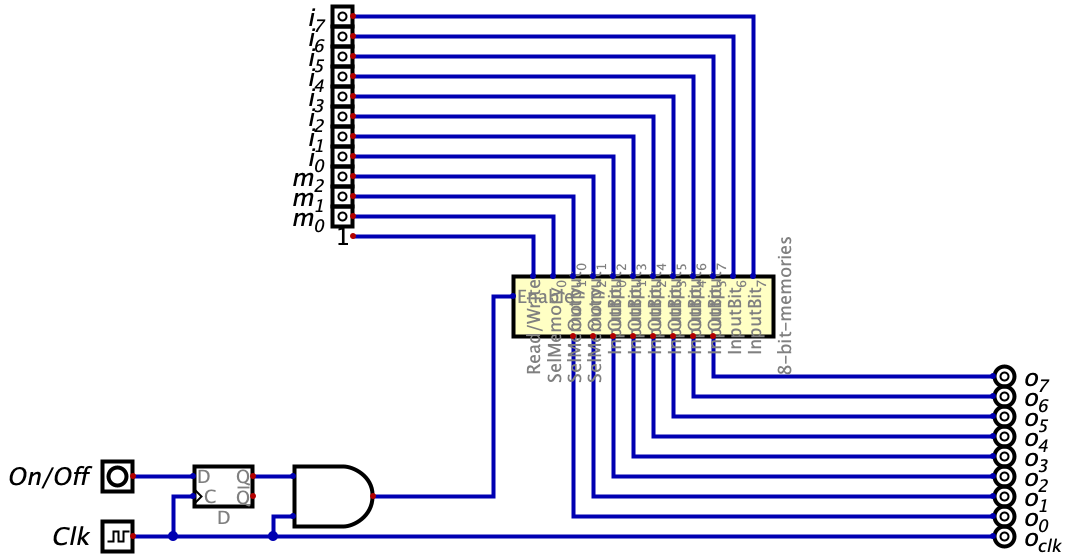
\includegraphics[width=0.5\textwidth]{assets/store_1bit.png}
    \caption{Implementation of the STORE instruction to one single memory.}
    \label{fig:store_1bit}
\end{figure}


Consider the case of storing data into any one of the three memories. The instruction circuit is shown in Figure~\ref{fig:store_3memories}.




\subsubsection{Load Instruction}

First, we implement the LOAD instruction from one single memory to one single register, ignoring all the unused parts.

To make the circuit work, we should first STORE some valid binary numbers then LOAD the numbers from the memory to a certain register.


Suppose that we have prepared the STORE and LOAD instructions in separate places. Ensuring the sequential order by applying a D Flip-Flop trigger, and connect to the memory block using a multiplexer to determine which block of memory should be 
visited depend on different instructions.

\begin{figure}[h!]
    \centering
    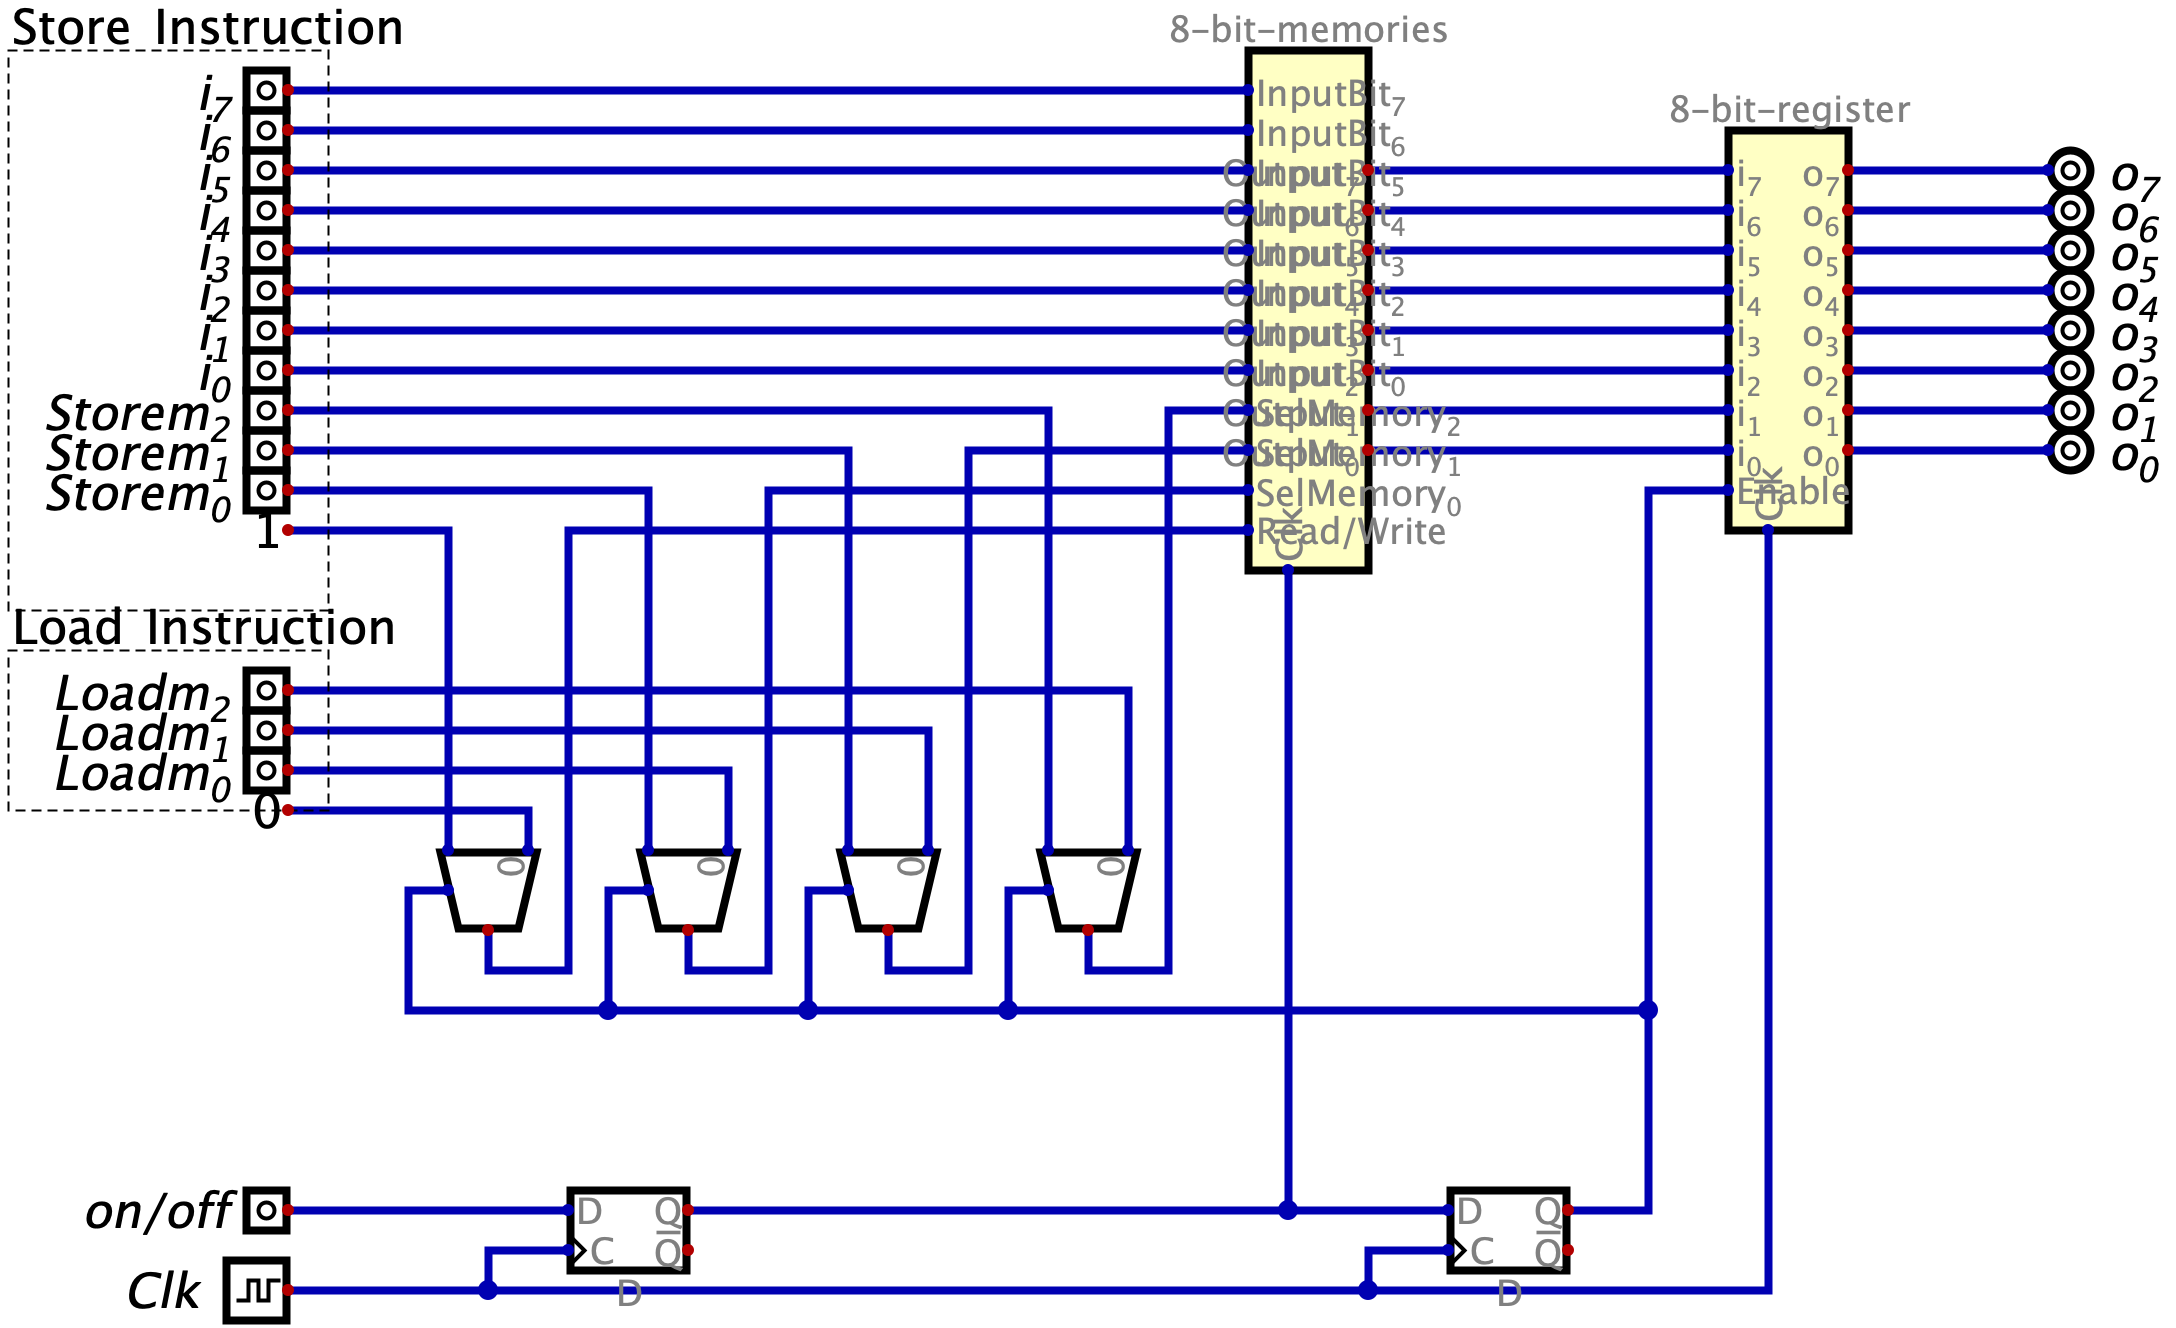
\includegraphics[width=0.5\textwidth]{assets/load.png}
    \caption{Implementation of the LOAD instruction from a single memory to a single register.}
    \label{fig:load}
\end{figure}


The implementation of the STORE and LOAD instructions to all of the memories and all of the registers is implemented in Figure~\ref{fig:load+store+3+2}.



\subsection{Question 10}

\subsubsection{Component: ALU}
First, we need to design the ALU. Since we have already implemented the 8-bits adder and a two's complement circuit, we could directly utilize them to implement the ALU.

The ALU that we have designed could perform addition and subtraction operations, we assume that binary numbers are stored in the form of two's complement, whether the number is in the register or in the memory.
The implementation is shown in Figure~\ref{fig:alu}, we utilize the two's complement component implemented in Figure~\ref{fig:twos_complement_course}. It's worthy to mention that the substraction of two binary numbers could be achieved by adding the two's complement of the second number to the first number. The ALU output the result in the form of two's complement.




\begin{figure}[h!]
    \centering
    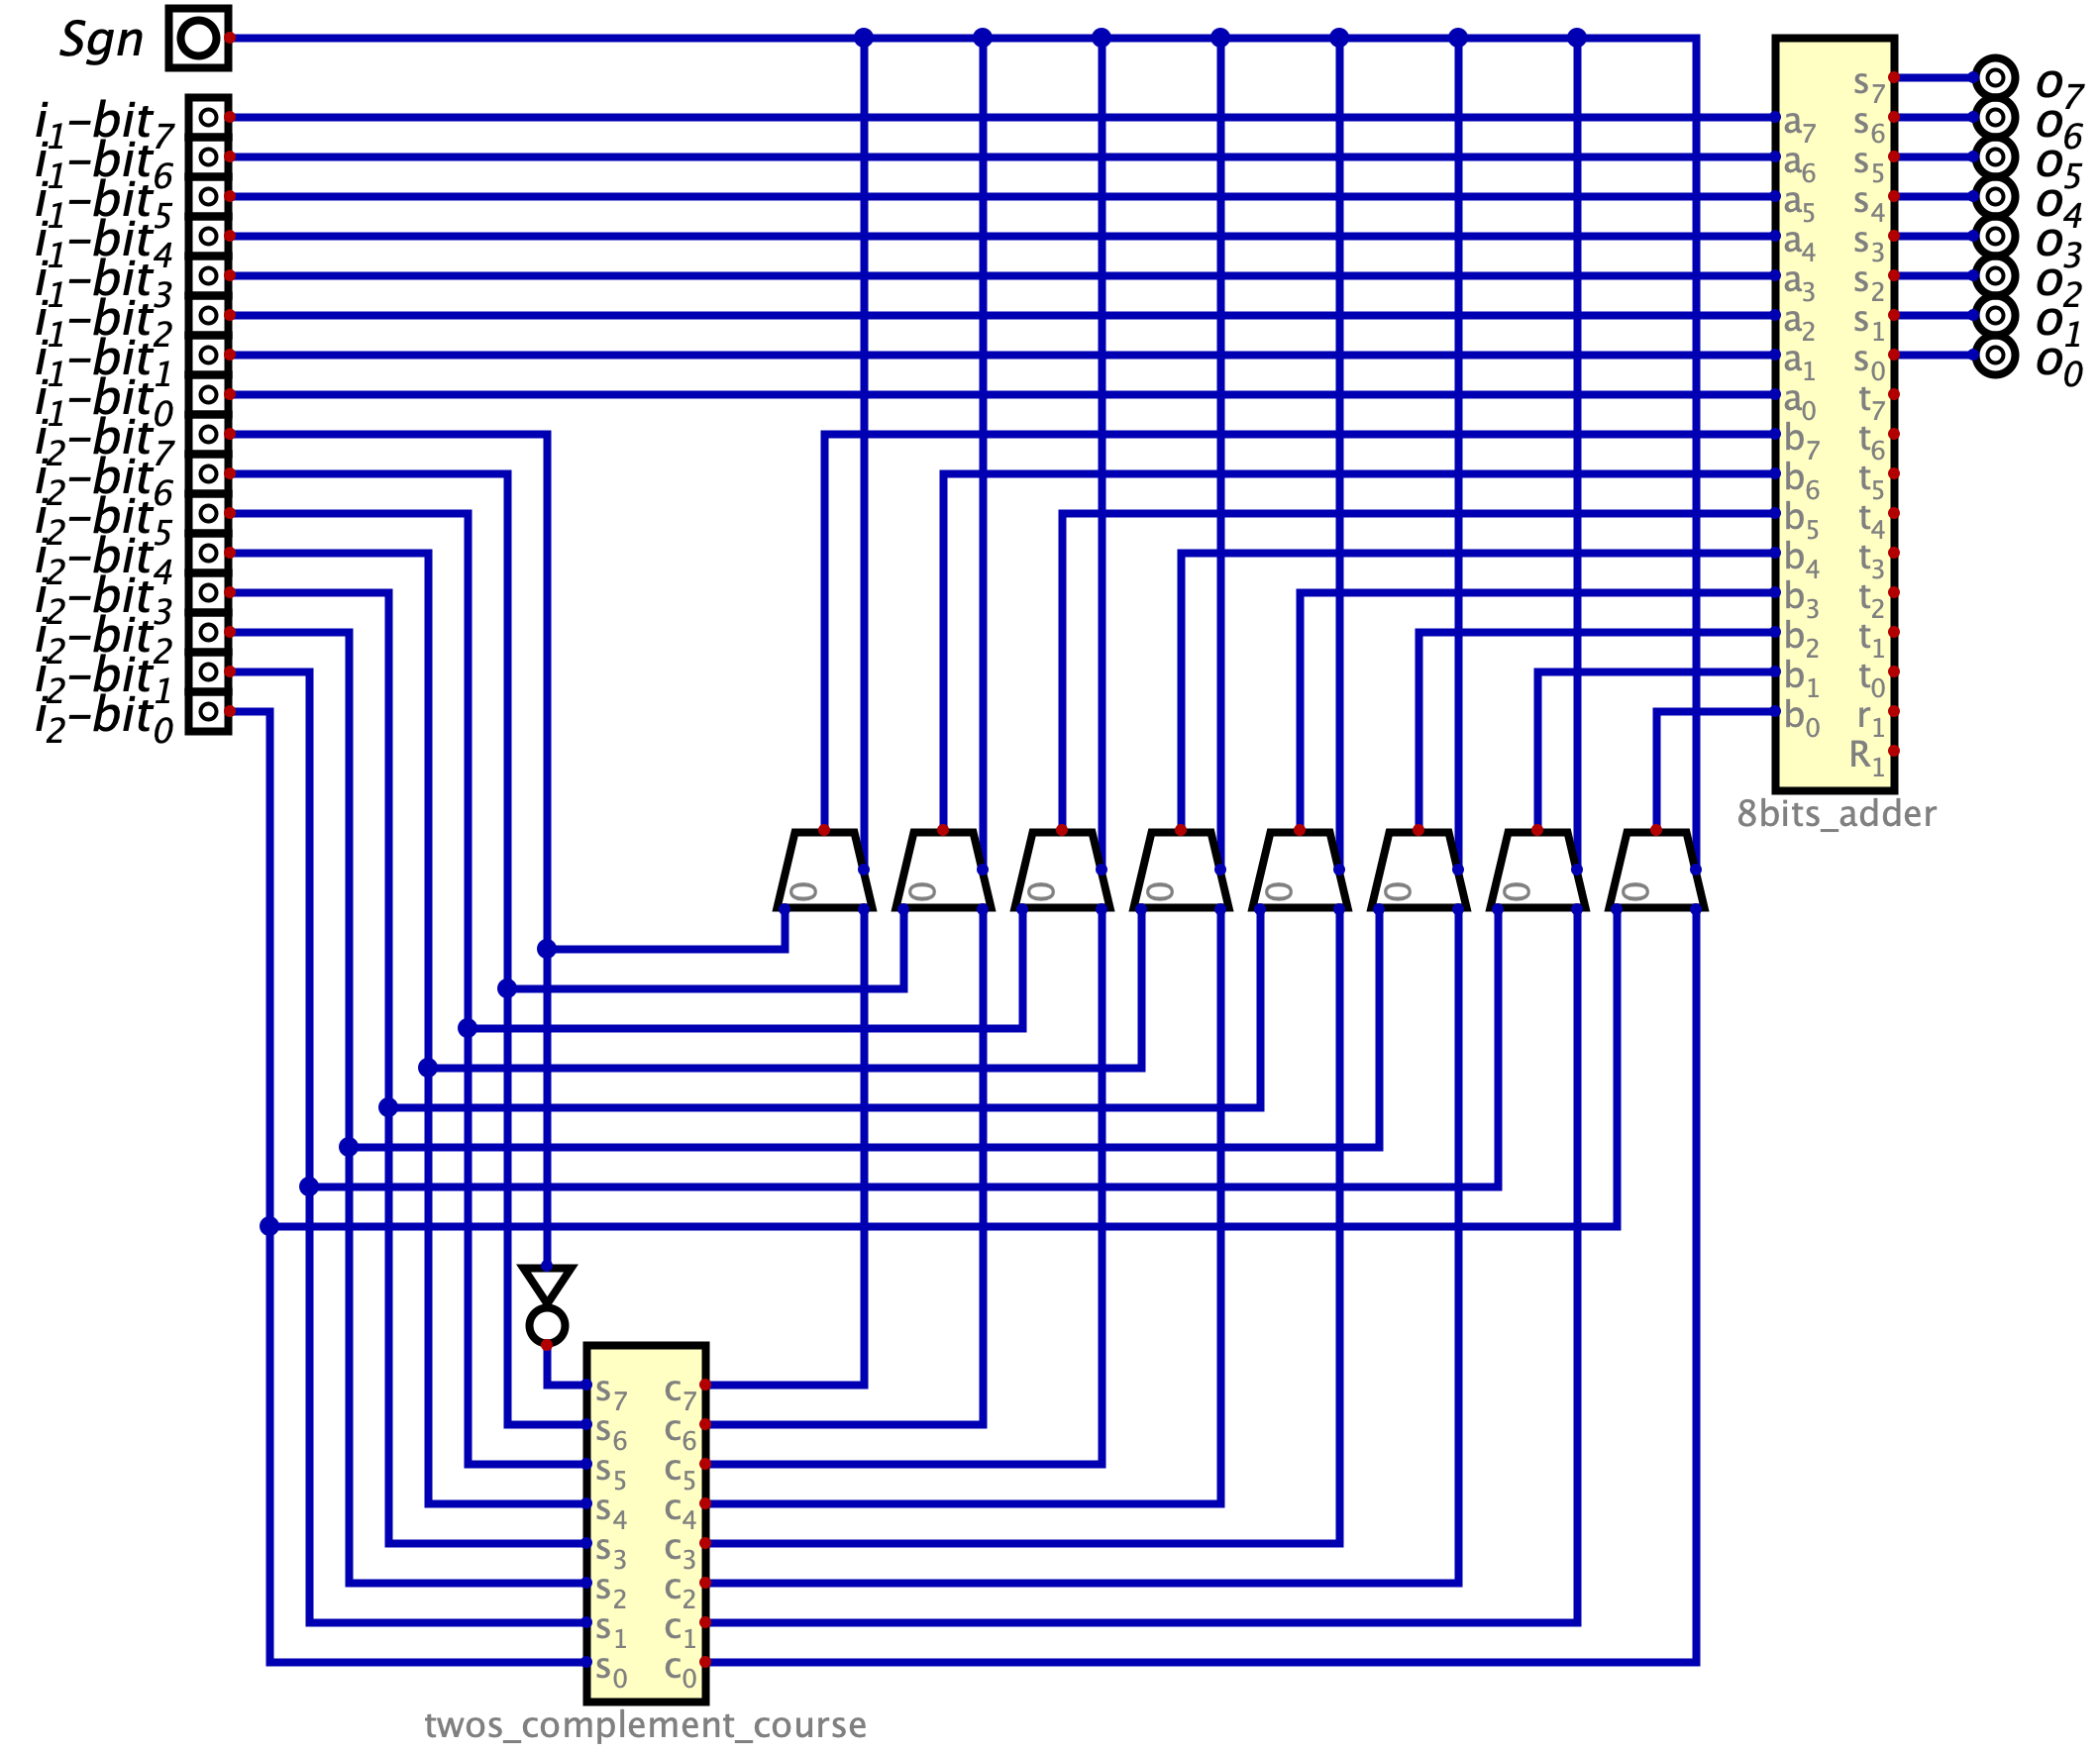
\includegraphics[width=0.5\textwidth]{assets/alu.png}
    \caption{Implementation of the ALU}
    \label{fig:alu}
\end{figure}

\subsubsection{Connections between components}

First and foremost, we must consider all the inter-connected components in the system. 

We would analyse the connections between the components in the following order:

\begin{itemize}
    \item \textit{Memory}: Input comes from the output of the Register or the given instruction, and the output is connected to the input of the Register.
    \item \textit{Register}: Input comes from the output of the Memory or the output of the ALU, and the output is connected to the input of the ALU or the input of the Memory.
    \item \textit{ALU}: Input comes from the output of the Register, and the output is connected to the input of the Register.
\end{itemize}

To select between different inputs, we need to use a multiplexer.

We divide the implementation into three steps. First, we implement the part of the memory, which is shown in Figure \ref{fig:all-instructions-1}.

\begin{figure}[h!]
    \centering
    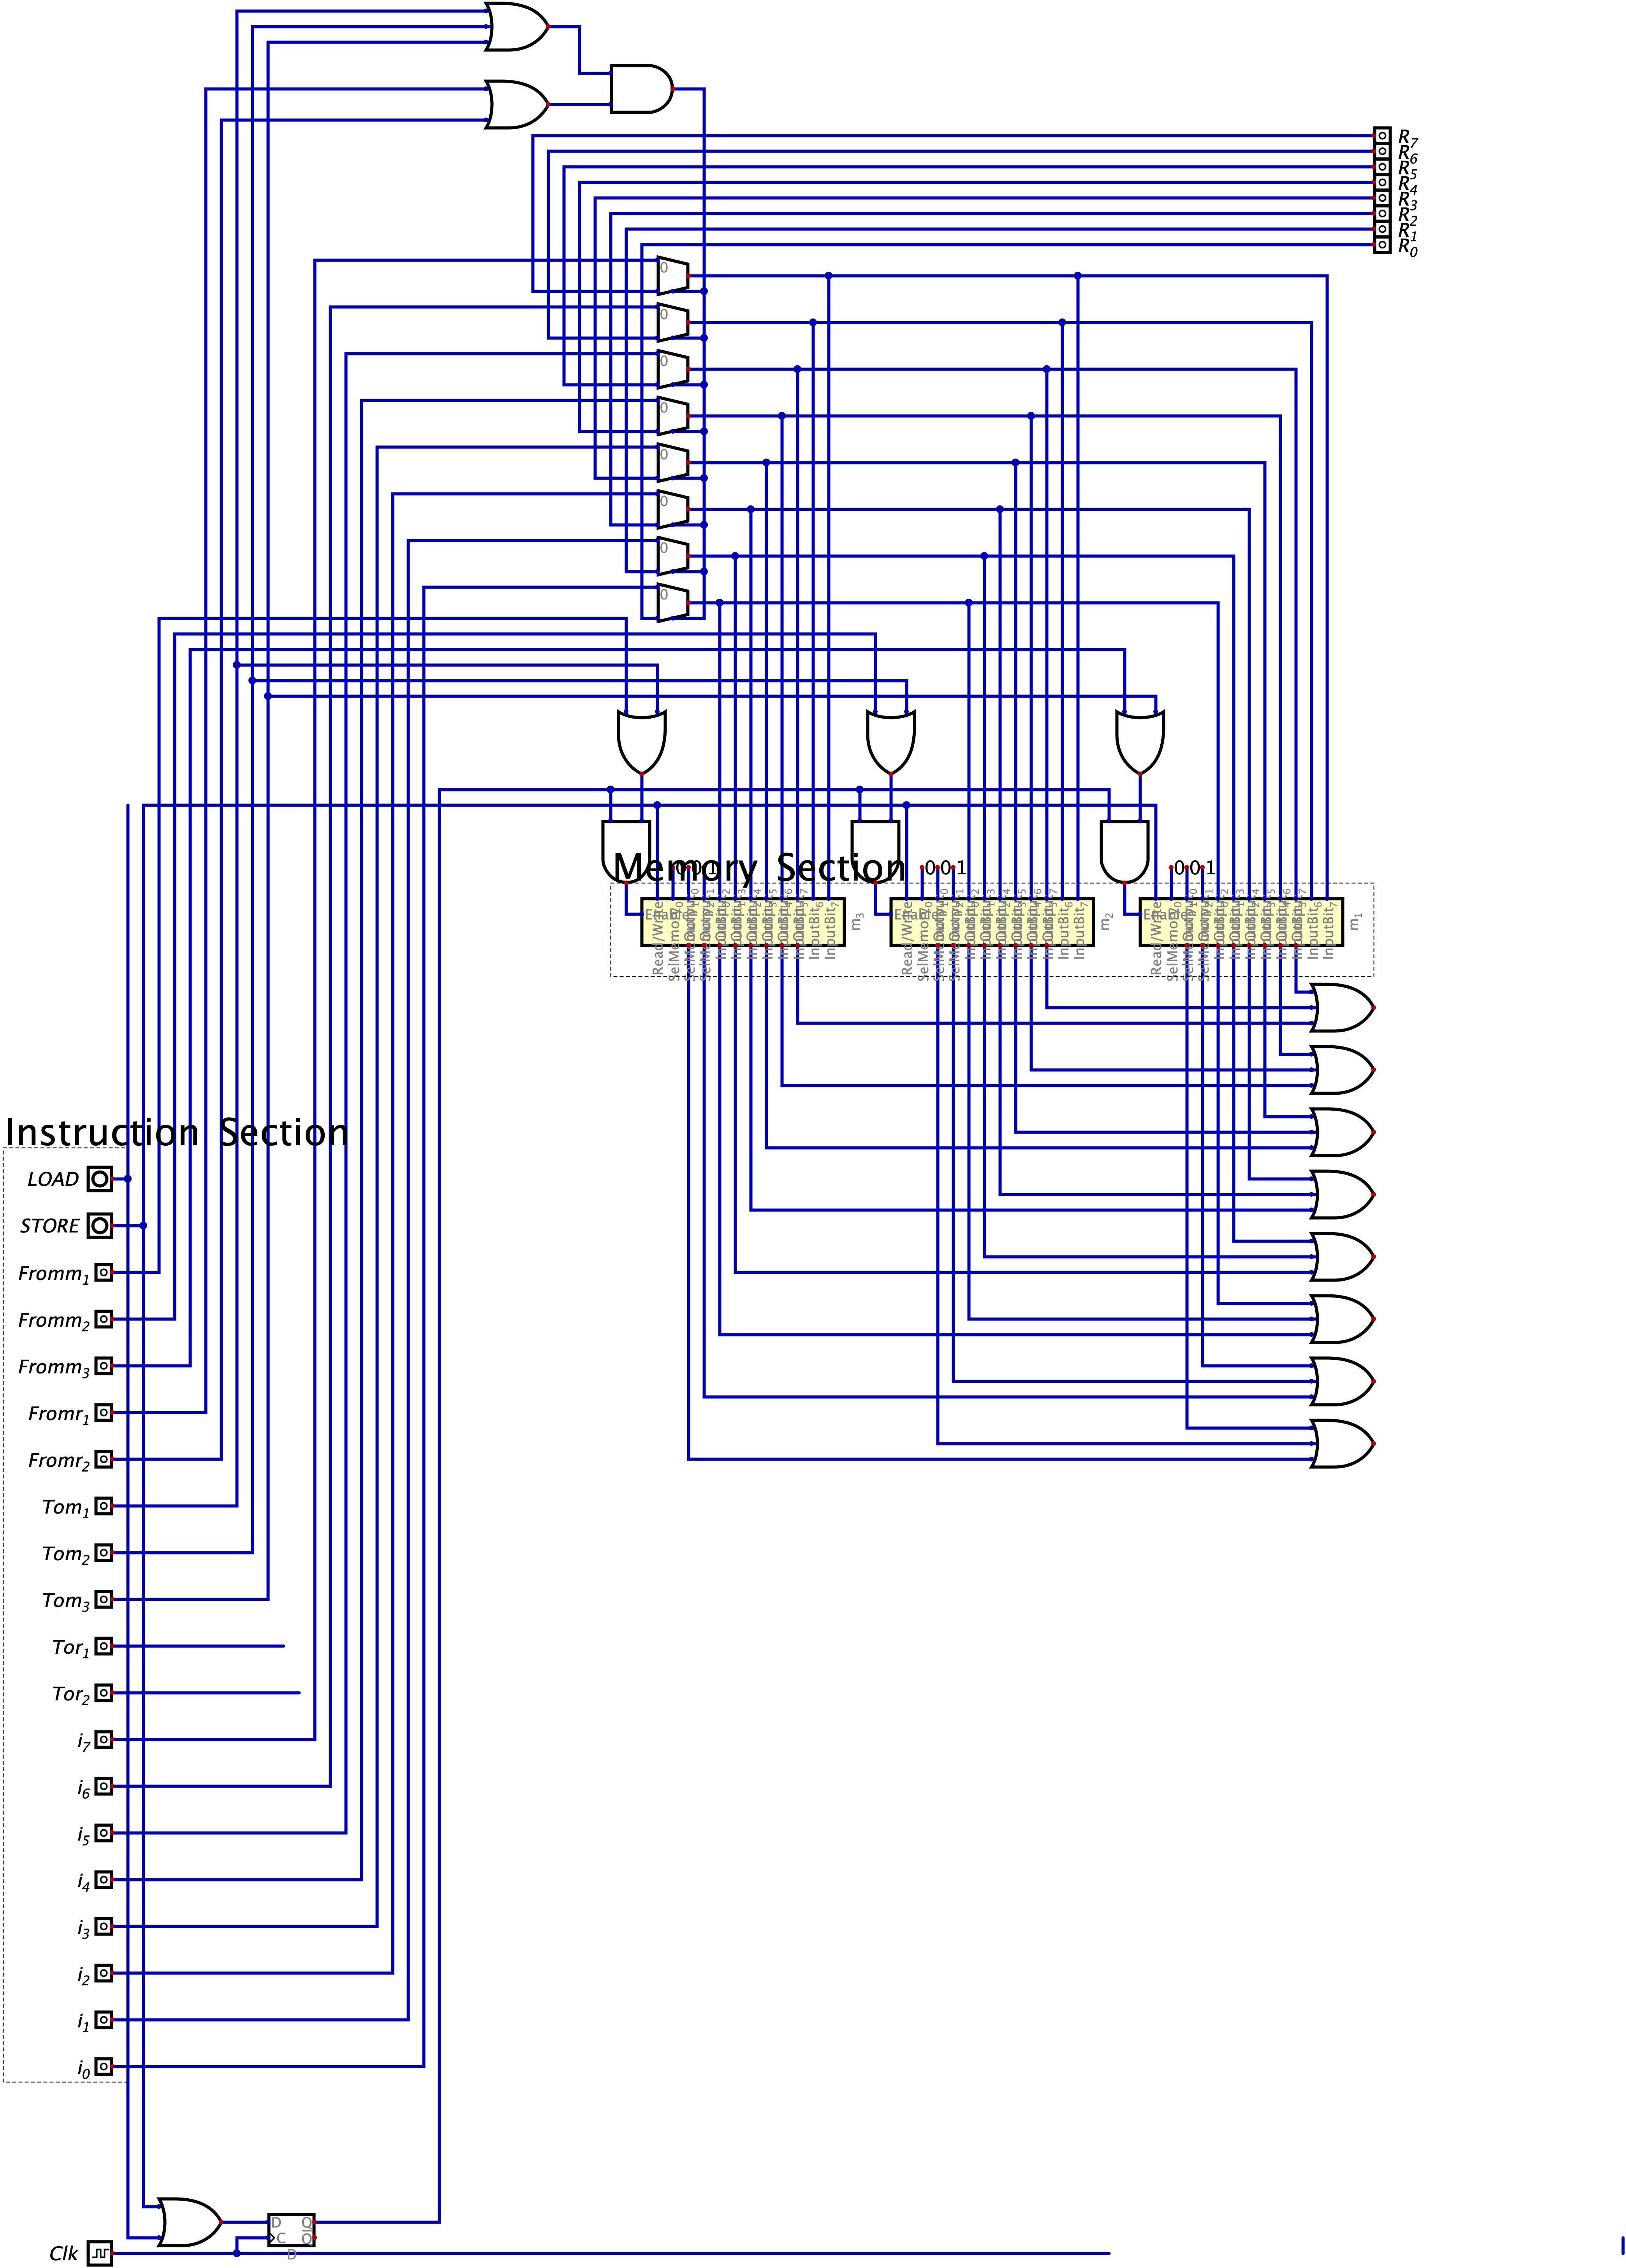
\includegraphics[width=0.5\textwidth]{assets/all-instructions-1.png}
    \caption{Implementation of all the instructions: Step 1}
    \label{fig:all-instructions-1}
\end{figure}

Then, we add the part of the register, which is shown in Figure \ref{fig:all-instructions-2}.

\begin{figure}[h!]
    \centering
    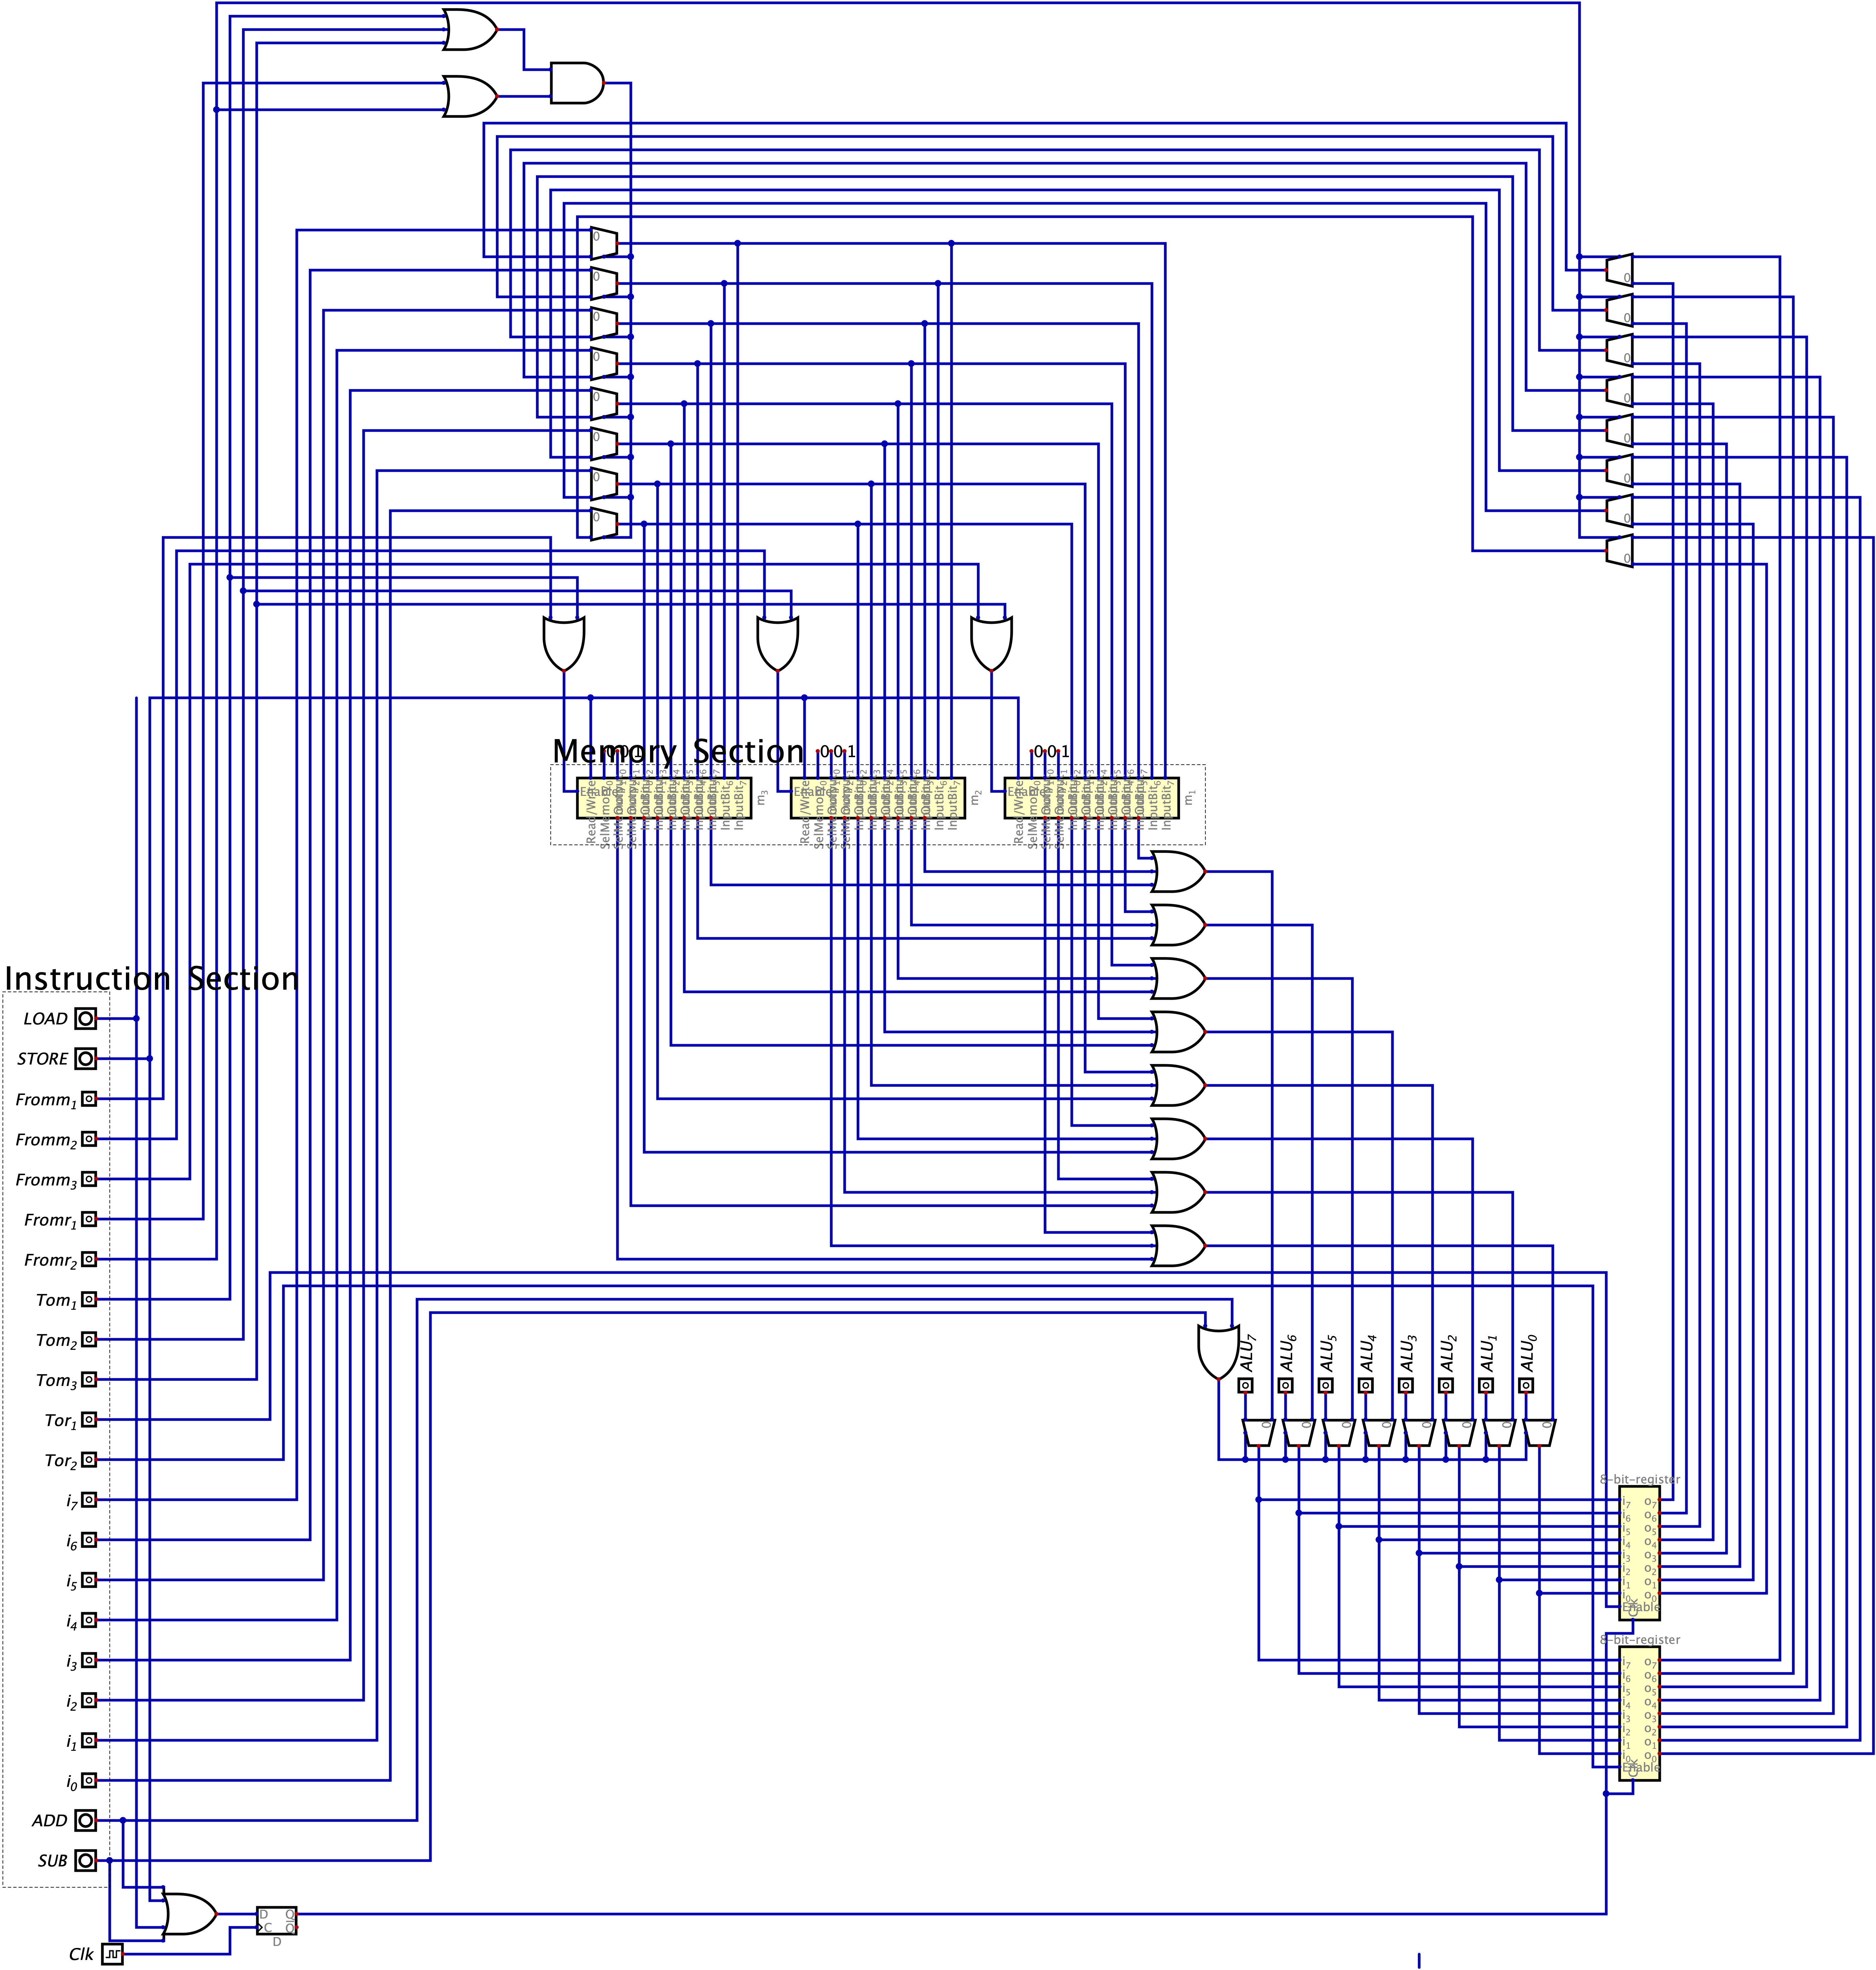
\includegraphics[width=0.5\textwidth]{assets/all-instructions-2.png}
    \caption{Implementation of all the instructions: Step 2}
    \label{fig:all-instructions-2}
\end{figure}

Finally, we add the part of the ALU with some tiny adjustments. The final version is shown in Figure \ref{fig:all-instructions-3}.


\textit{How to use the circuit:}

\begin{enumerate}
    \item Though it is not mentioned in the question, the numbers has to be first stored into the memories, then they could be fetched by registers. Thus, we must store the two 8-bits binary numbers into the memories.
    \textit{How to store the numbers?} For example, you would like to store the number 15 to the first memory block, you should set the input of $i_3$, $i_2$, $i_1$, $i_0$ and $\text{To}m_1$ to 1 and left the others 0. Then, (note: these two steps should be done in sequence) set the input of STORE to 1. Similarly, if you want to store a number to the second memory, set the $\text{To}m_2$ to 1 then press the STORE button.

    \item Afterwards, we should LOAD the numbers from the memories to the registers. For example, now we want to fetch the data from the first memory block to the first register. Before everything, clean up the former input. Then, set the input of $\text{From}m_1$ and $\text{To}r_1$ to 1 and left the others 0. After that, set the input of LOAD to 1.
    \item To subtract the two numbers, set up the register that you wish to store the result. For example, if we want to store the result into the second register, we should set the input of $\text{To}r_2$ to 1 and left the others 0. Then, set the input of SUB to 1.

    \item Finally, we should store the result into the memory. For example, if we want to store the result into the third memory block, set the input of $\text{From}r_2$ and $\text{To}m_3$ to 1 and left the others 0. Then, set the input of STORE to 1.

\end{enumerate}



\begin{figure*}[h!]
    \centering
    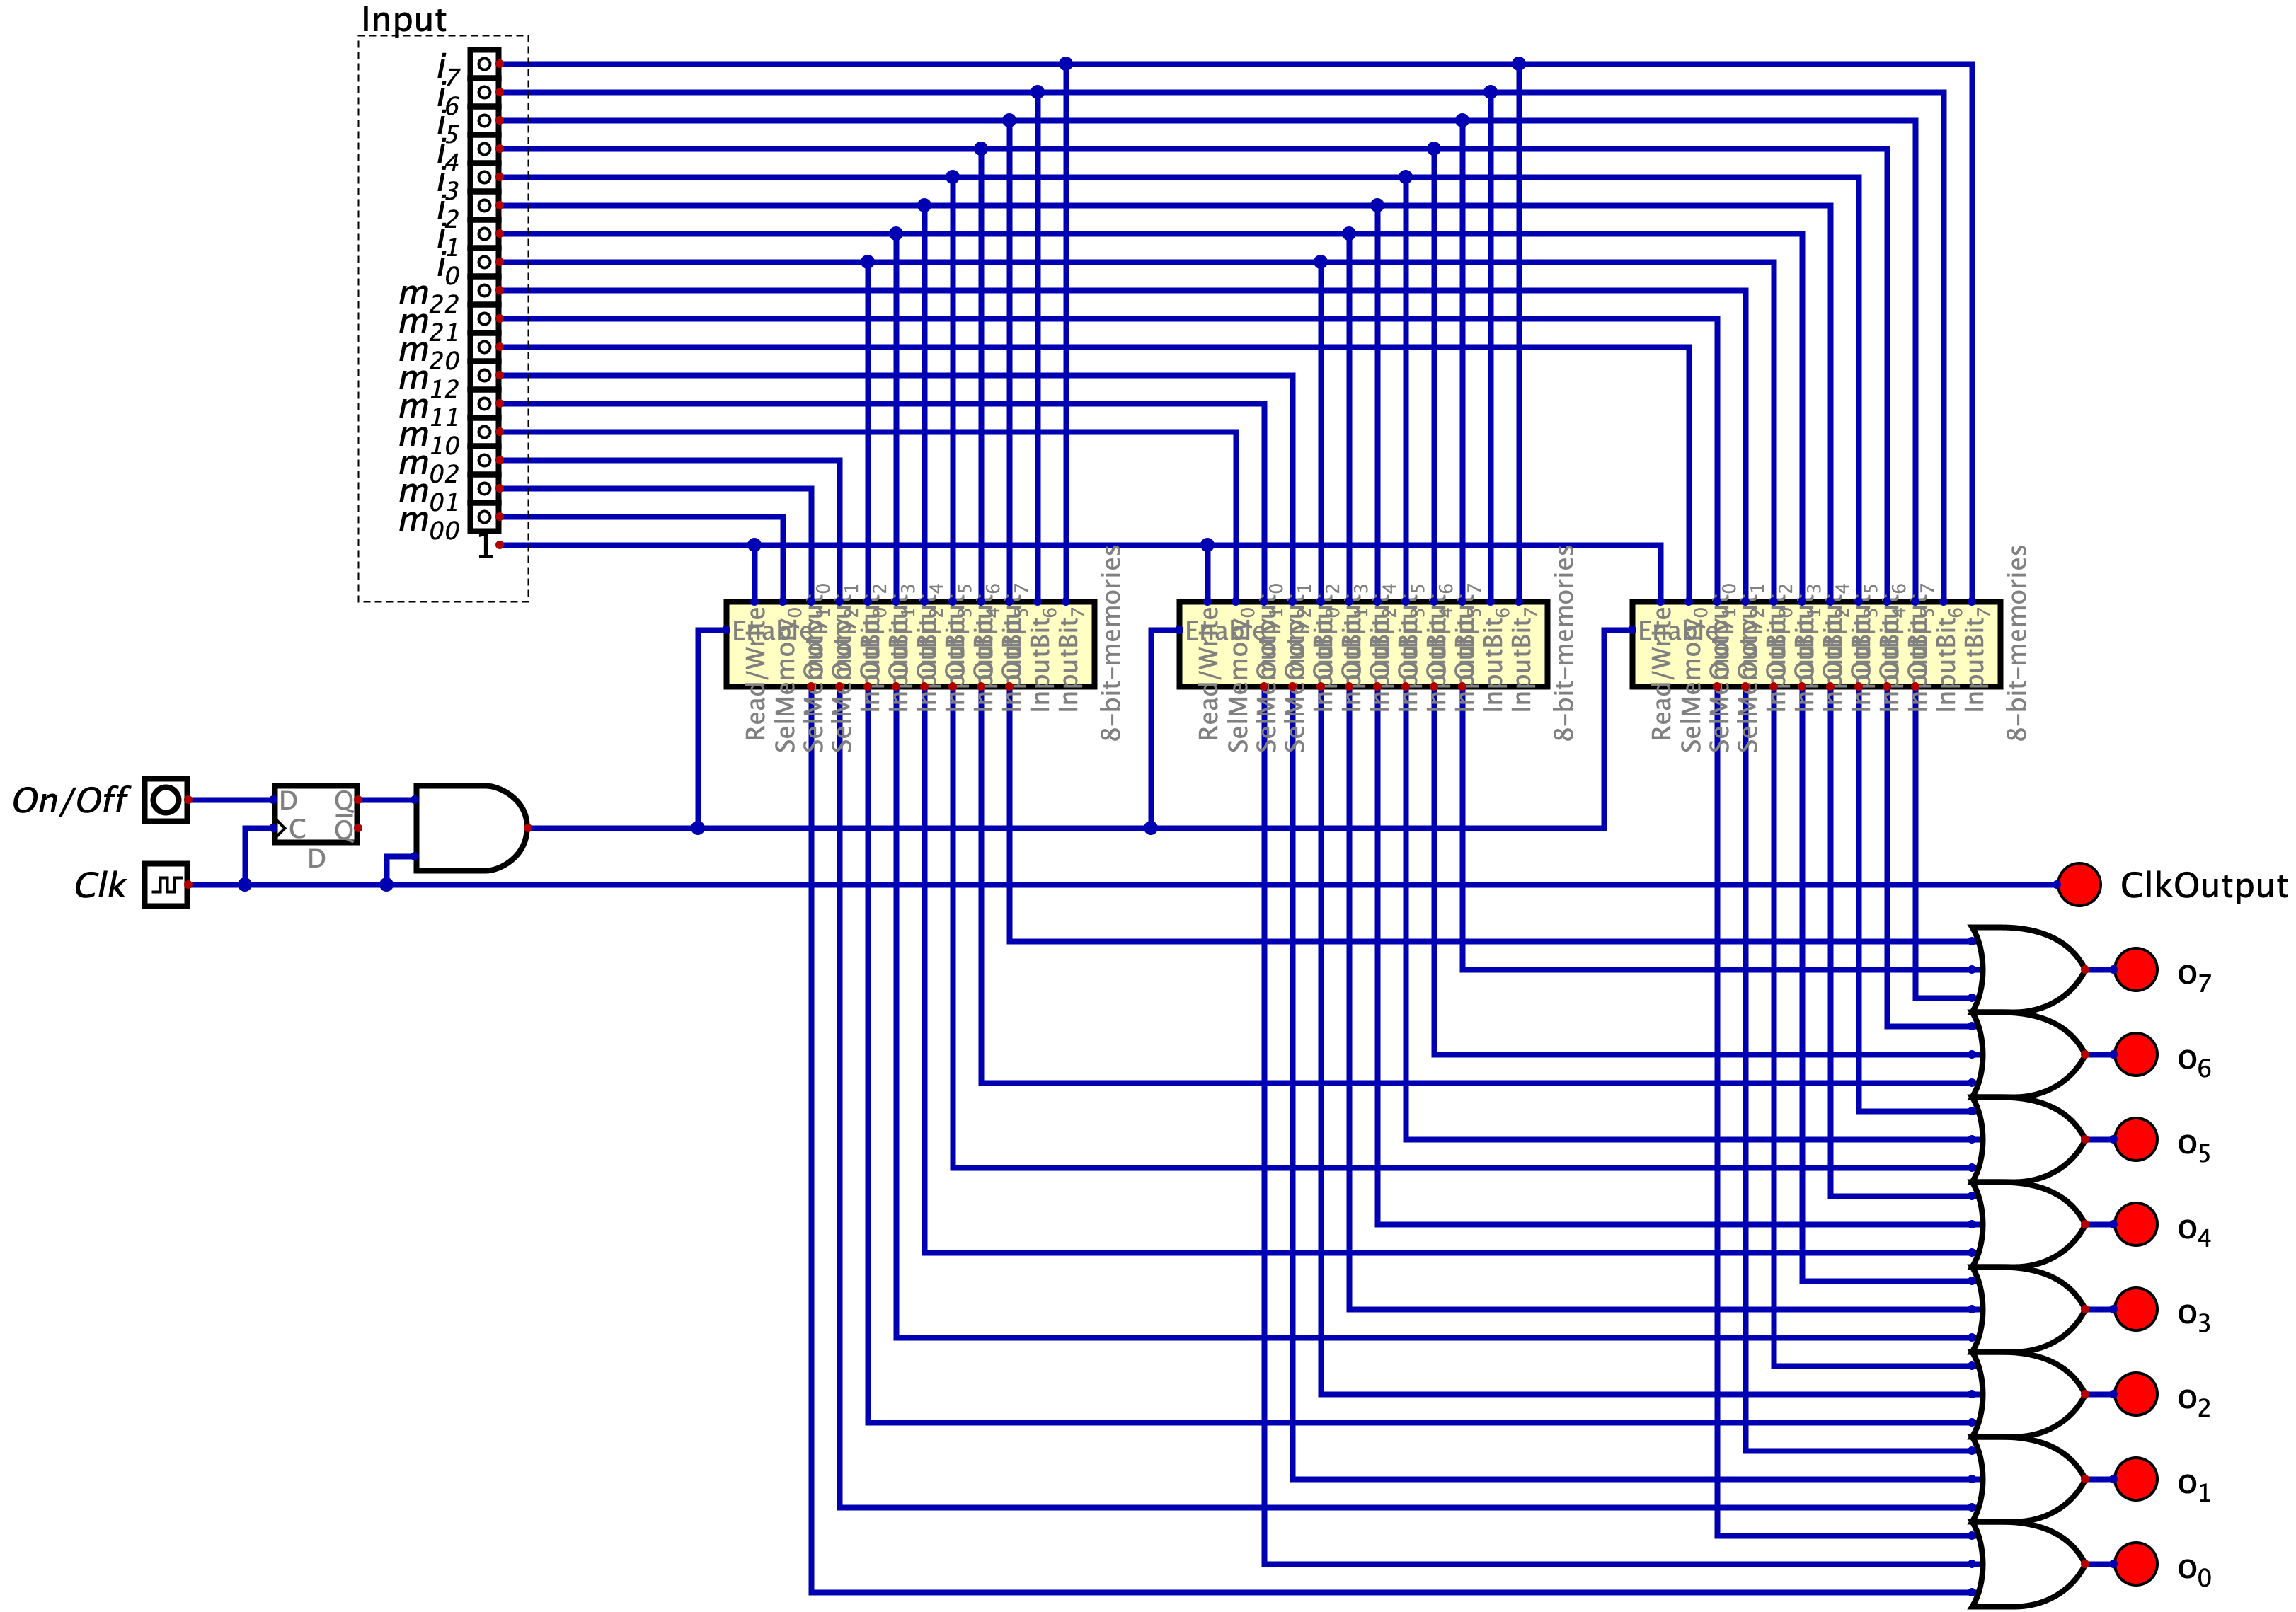
\includegraphics[width=\textwidth]{assets/store.png}
    \caption{Implementation of the STORE instruction to all of the memories.}
    \label{fig:store_3memories}
\end{figure*}

\begin{figure*}[h!]
    \centering
    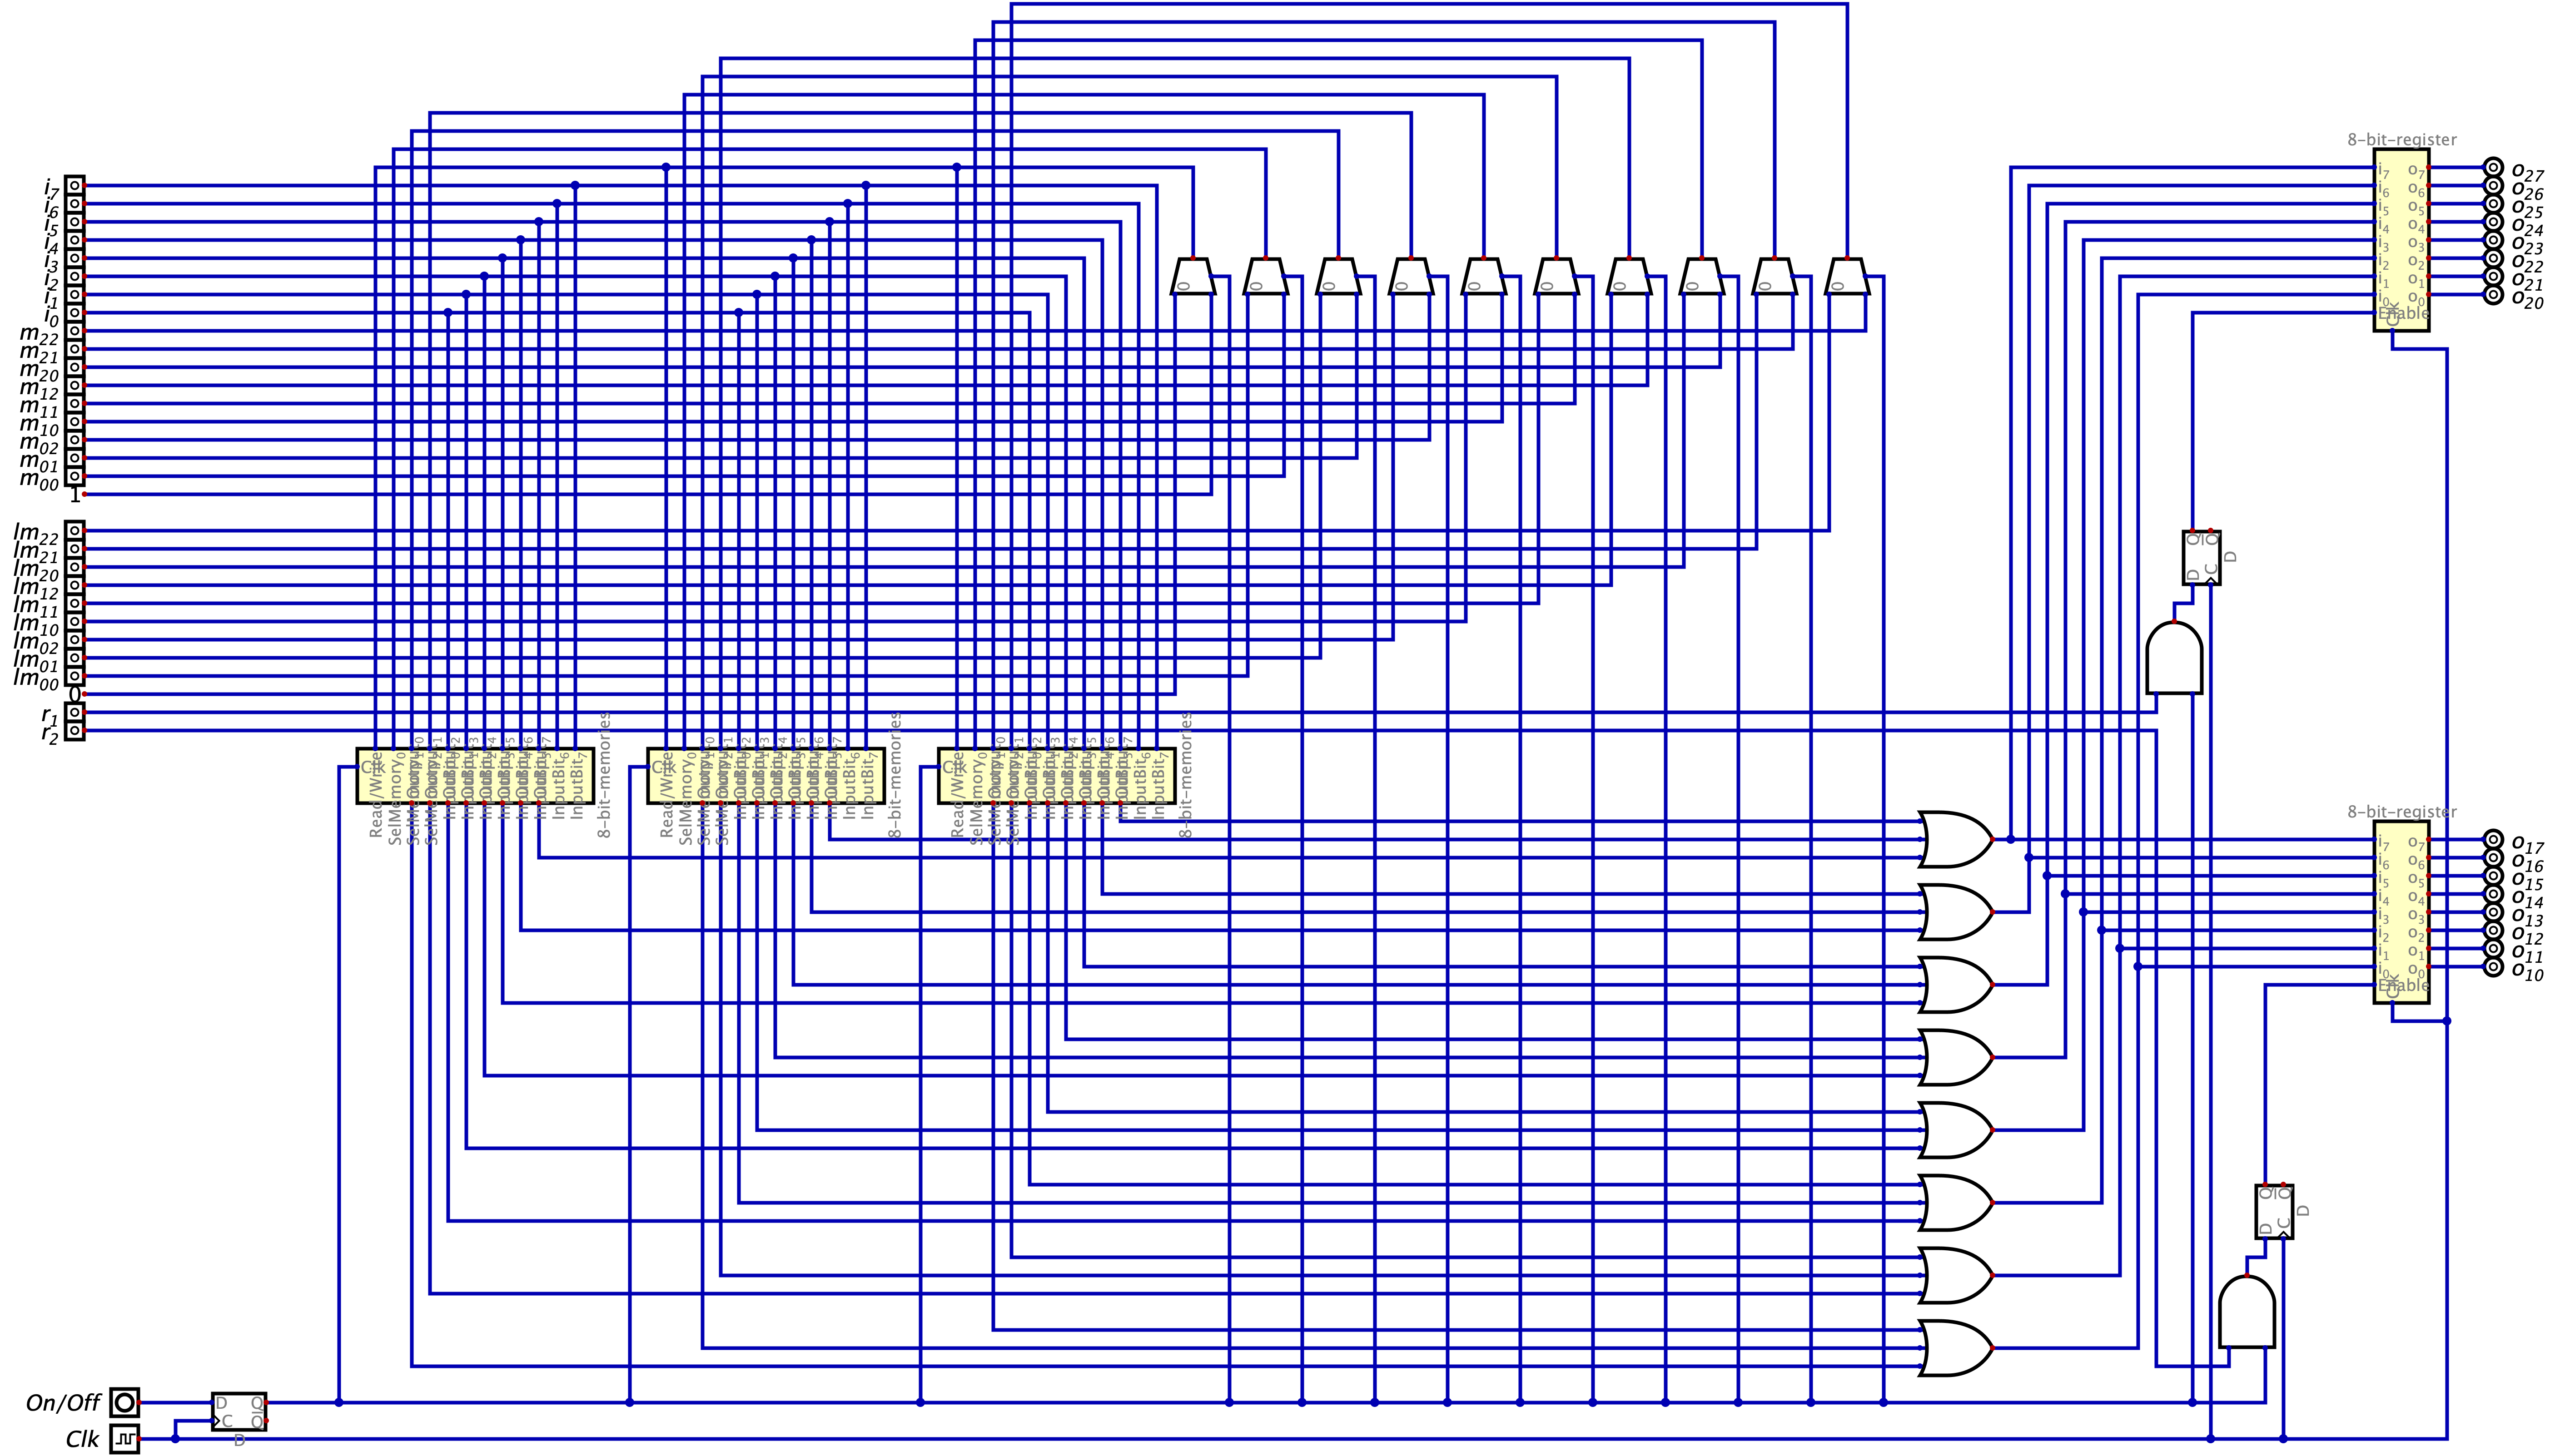
\includegraphics[width=\textwidth]{assets/load+store+3+2.png}
    \caption{Implementation of the LOAD instruction to all of the memories and all of the registers.}
    \label{fig:load+store+3+2}
\end{figure*}

\begin{figure*}[h!]
    \centering
    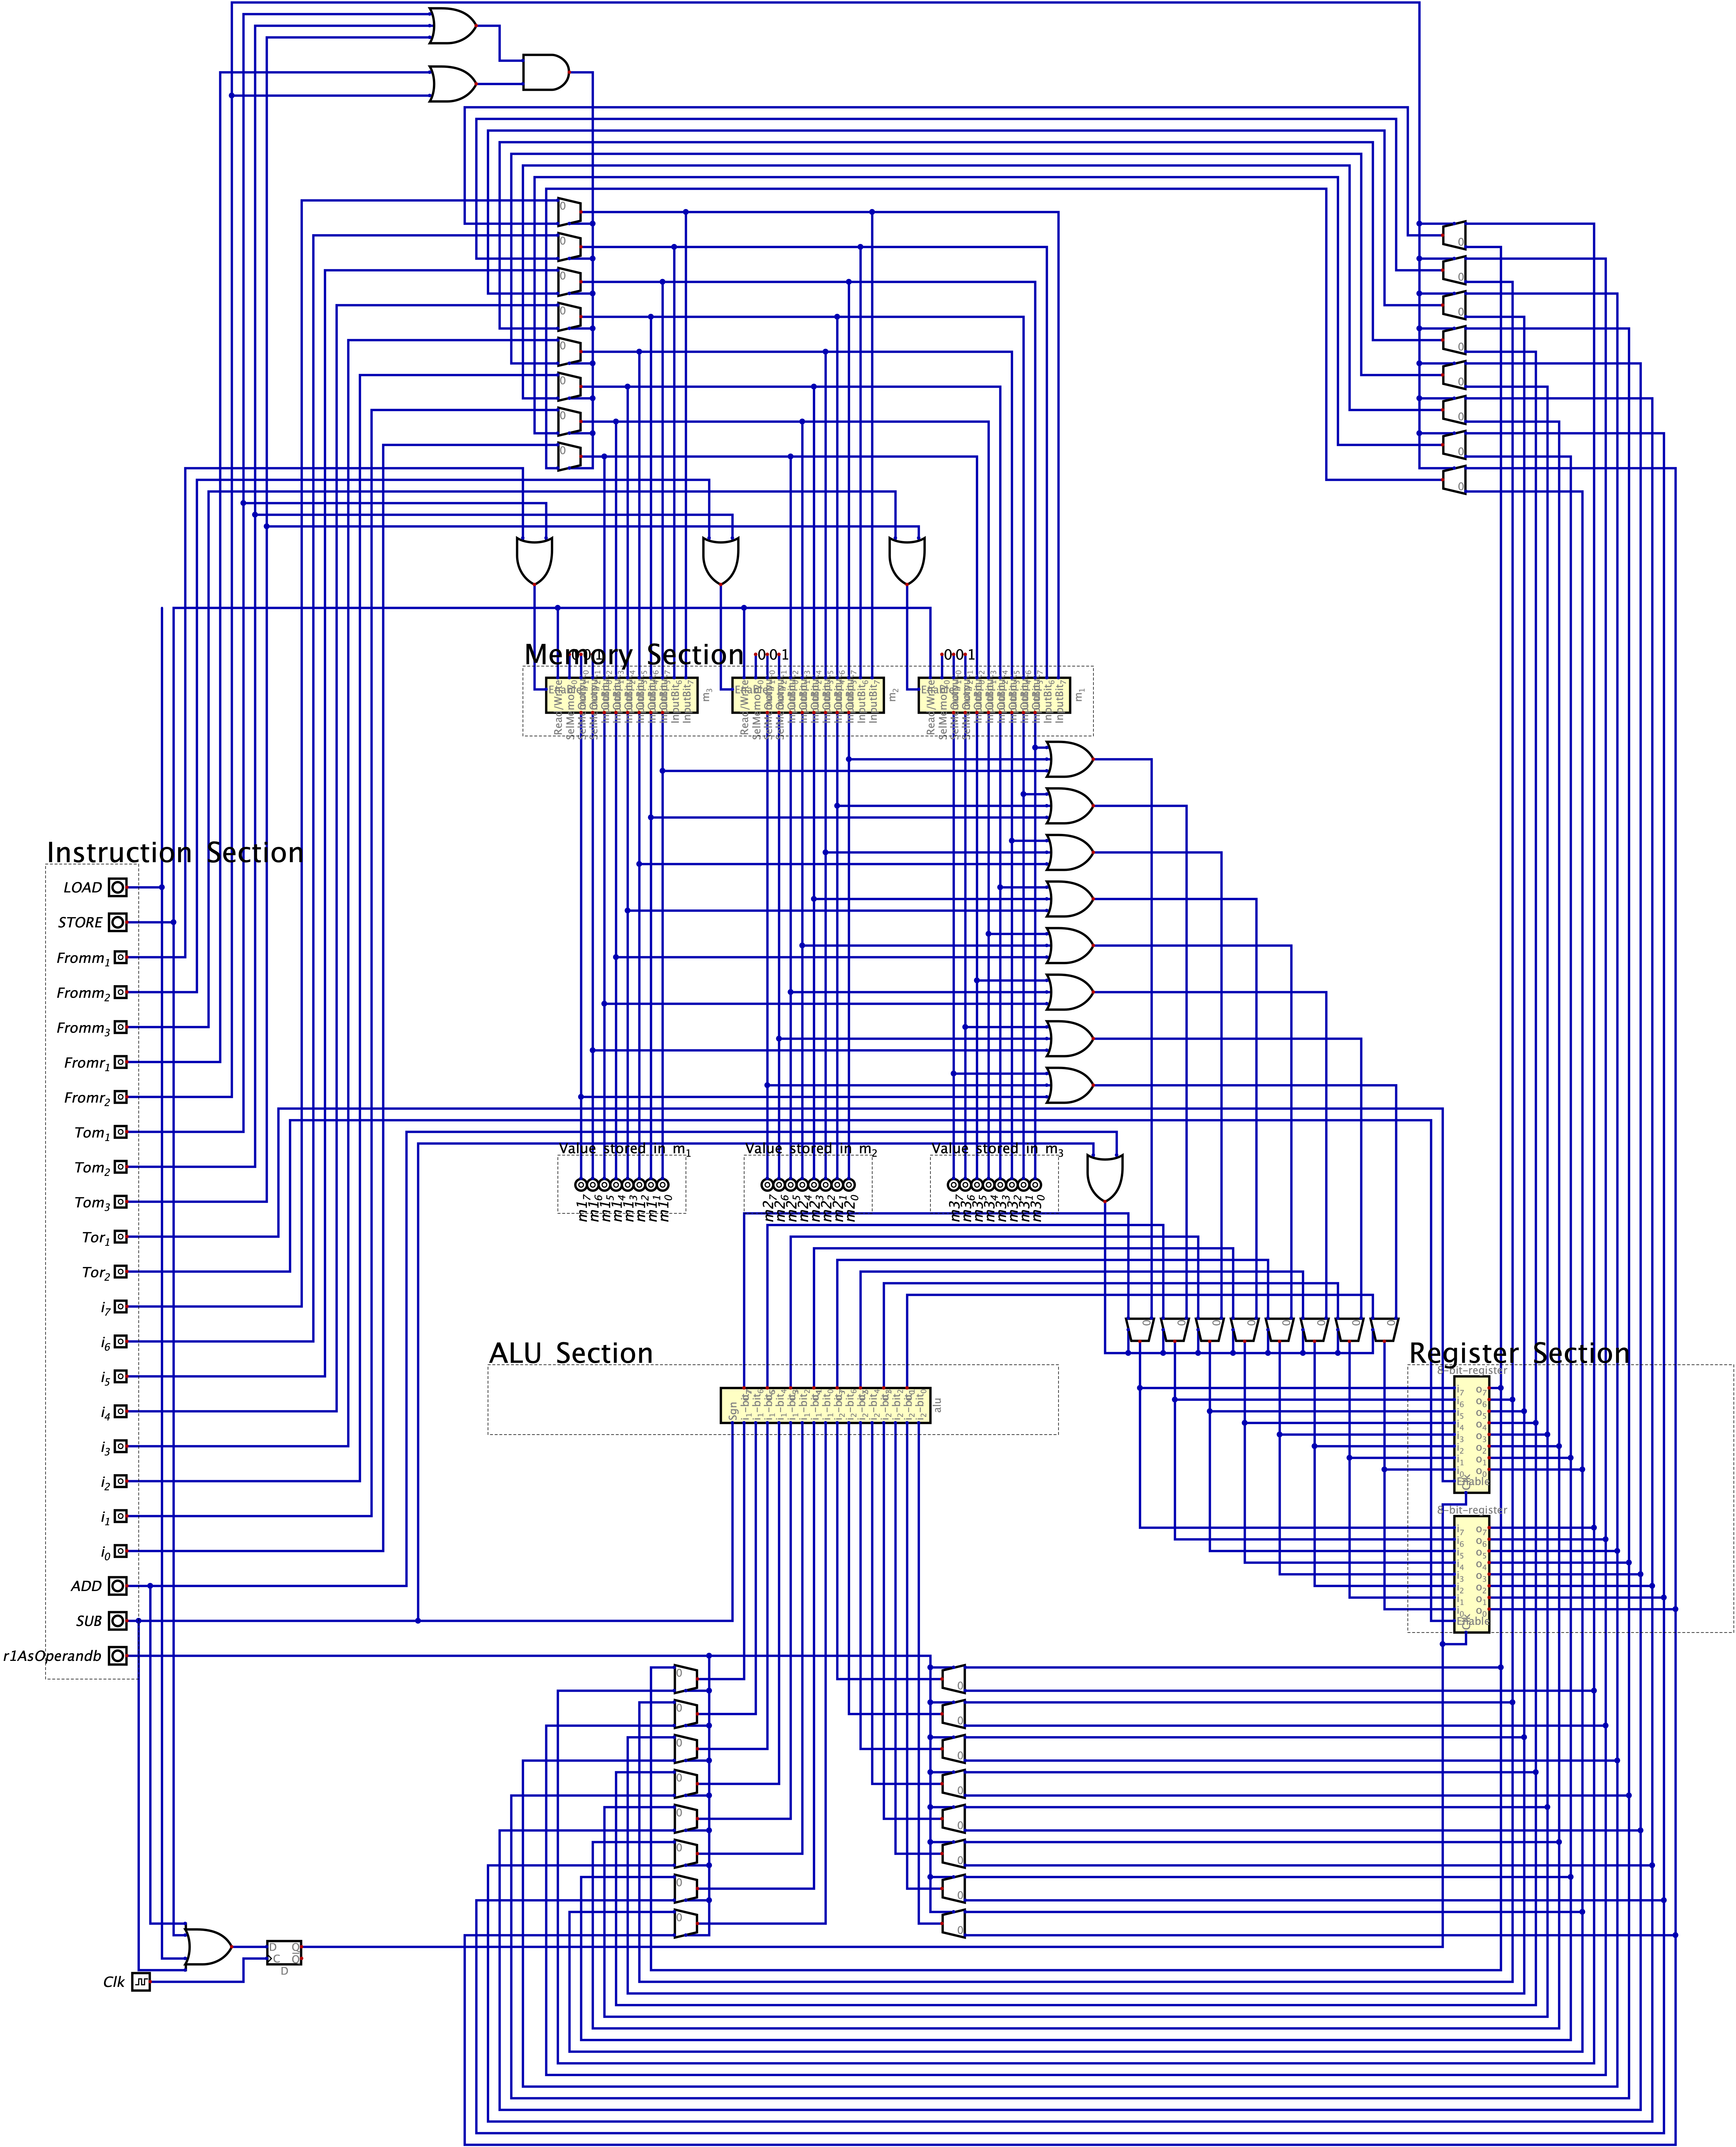
\includegraphics[width=\textwidth]{assets/all-instructions.png}
    \caption{Implementation of all the instructions}
    \label{fig:all-instructions-3}
\end{figure*}

\end{document}
